%
% Kittel_Kroemer_Thermal_Physics.tex 
%
\documentclass[twoside]{amsart}
\usepackage{amssymb,latexsym}
\usepackage{times}
\usepackage{graphics}
\usepackage{listings}
\usepackage{hyperref}
\hypersetup{colorlinks=true, urlcolor=blue}
\usepackage{tikz}

\usetikzlibrary{matrix,arrows}

\usepackage[version=3]{mhchem}

%\usepackage{graphics}

\oddsidemargin-0.15cm
\evensidemargin-0.15cm
\topmargin-1.8cm     %I recommend adding these three lines to increase the 
\textwidth17.5cm   %amount of usable space on the page (and save trees)
\textheight24.5cm  
\parindent0.0em

%This next line (when uncommented) allow you to use encapsulated
%postscript files for figures in your document
%\usepackage{epsfig}

%plain makes sure that we have page numbers
\pagestyle{plain}

\theoremstyle{plain}
\newtheorem{theorem}{Theorem}
\newtheorem{axiom}{Axiom}
\newtheorem{lemma}{Lemma}
\newtheorem{proposition}{Proposition}

\theoremstyle{definition}
\newtheorem{definition}{Definition}

\title{Notes and Solutions to \emph{ Thermal Physics } by Charles Kittle and Herbert Kroemer }

\author{
  Ernest Yeung - Los Angeles
       }
\date{Fall 2008}

\email{ernestyalumni@gmail.com}
\urladdr{http://ernestyalumni.wordpress.com}
\thanks{I am crowdfunding on Tilt/Open to support basic sciences research: \url{ernestyalumni.tilt.com}.  If you find this pdf (and LaTeX file) valuable and/or helpful, please consider donating to my crowdfunding campaign. There is also a Paypal button there and it's easy to donate with PayPal, as I had recently to the Memorial Fund for the creator of Python's matplotlib.  But the most important thing is for anyone, anywhere, and at anytime be able to learn thermodynamics and use it for research and application and so I want to keep this as openly public as possible, in the spirit of open-source software.  Tilt/Open is an open-source crowdfunding platform that is unique in that it offers open-source tools for building a crowdfunding campaign.  Tilt/Open has been used by Microsoft and Dick’s Sporting Goods to crowdfund their respective charity causes.} 


%This defines a new command \questionhead which takes one argument and
%prints out Question #. with some space.
\newcommand{\questionhead}[1]
  {\bigskip\bigskip
   \noindent{\small\bf Question #1.}
   \bigskip}

\newcommand{\problemhead}[1]
  {
   \noindent{\small\bf Problem #1.}
   }

\newcommand{\exercisehead}[1]
  {
   \noindent{\small\bf Exercise #1.}
   \smallskip}

\newcommand{\solutionhead}[1]
  {
   \noindent{\small\bf Solution #1.}
   }


%-----------------------------------
\begin{document}
%-----------------------------------
\definecolor{darkgreen}{rgb}{0,0.4,0}
\lstset{language=Python,
 frame=bottomline,
 basicstyle=\scriptsize,
 identifierstyle=\color{blue},
 keywordstyle=\bfseries,
 commentstyle=\color{darkgreen},
 stringstyle=\color{red},
 }


\begin{abstract}
These are notes and solutions to Kittle and Kroemer's \textbf{Thermal Physics}.  The solutions are (almost) complete: I will continuously add to subsections, before the problems in each chapter, my notes that I write down as I read (and continuously reread).  

I am attempting a manifold formulation of the equilibrium states in the style of Schutz's \textbf{Geometrical Methods of Mathematical Physics} and will point out how it applies directly to \textbf{Thermal Physics}.  Other useful references along this avenue of investigation is provided at the very bottom in the references.  

Any and all feedback, including negative feedback, is welcomed and you can reach me by email or my \href{http://ernestyalumni.wordpress.com}{wordpress.com blog}.  

You are free to copy, edit, paste, and add onto the pdf and LaTeX files as you like in the spirit of open-source software.  You are responsible adults to use these notes and solutions as governed by the Caltech Honor Code: ``No member of the Caltech community shall take unfair advantage of any other member of the Caltech community'' and follow the Honor Code in spirit.   

\end{abstract}


\maketitle

\textsc{Second Edition}.  \textbf{Thermal Physics}.  Charles Kittel.  Herbert Kroemer.  W. H. Freeman and Company.  New York.  QC311.5.K52 1980  536'.7  ISBN 0-7167-1088-9

\section{States of a Model System}

\section{Entropy and Temperature}

\subsection*{Thermal Equilibrium}

EY : 20150821 Based on considering the physical setup of two systems that can only exchange energy between each other, that are in thermal contact, this is a derivation of temperature.

$U = U_1 + U_2$ is constant total energy of 2 systems $1,2$ in thermal contact \\
multiplicity $g(N,U)$ of combined system is 
\[
g(N,U) = \sum_{U_1 \leq U} g_1(N_1,U_1)g_2(N_2,U-U_1)
\]
The ``differential'' of $g(N,U)$ is 
\[
dg = \left( \frac{\partial g_1}{ \partial U_1 } \right)_{N_1} g_2 dU + g_1\left( \frac{\partial g_2 }{ \partial U_2 } \right)_{N_2} dU_2 = 0 
\]
EY : 20150821 This step can be made mathematically sensible by considering the exterior derivative $d$ of $g \in C^{\infty}(\Sigma)$, where $\Sigma$ is the manifold of states of the system, with local coordinates $N,U$, where $U$ happens to be a global coordinate. Then, consider a curve in $\Sigma$ s.t. it has no component in $\frac{\partial}{ \partial N}$, $\frac{\partial}{ \partial N_1}$, and this curve is a ``null curve'' so that the vector field $X\in \mathfrak{X}(\Sigma)$ generated by this curve is s.t. $dg(X)=0$.  

With $-dU_1 = dU_2$,
\[
\frac{1}{g_1} \left( \frac{\partial g_1}{ \partial U_1}\right)_{N_1} = \frac{1}{g_2} \left( \frac{\partial g_2}{ \partial U_2} \right)_{N_2} \Longrightarrow \left( \frac{ \partial \ln{g_1} }{ \partial U_1} \right)_{N_1} = \left( \frac{ \partial \ln{g_2}}{ \partial U_2} \right)_{N_2}
\]
Define
\[
\sigma(N,U) := \ln{ g(N,U)}
\]
Then
\[
\Longrightarrow \left( \frac{ \partial \sigma_1}{ \partial U_1} \right)_{N_1} = \left( \frac{ \partial \sigma_2}{ \partial U_2} \right)_{N_2}
\]



\subsection*{Temperature}

$T_1=T_2$ - temperatures of 2 systems in thermal equilibrium are equal.  

$T$ ``must be a function of $ \left( \frac{ \partial \sigma}{ \partial U} \right)_N$ \cite{CKittleHKroemer}.  
\[
\Longrightarrow \frac{1}{T} = k_B \left( \frac{ \partial \sigma }{ \partial U} \right)_N
\]
Experimentally, $k_B = 1.381 \times 10^{-23} \, J/K = 1.381\times 10^{-16} \, \text{ ergs}/ K$.  

Now 
\[
\begin{gathered}
\frac{1}{\tau} = \left( \frac{ \partial \sigma }{ \partial U} \right)_N
\tau = k_B T
\end{gathered}
\]


\subsection*{Problems}

\solutionhead{1} \textbf{Entropy and temperature}.  
\begin{itemize}
\item[(a)] Recall that $\frac{1}{\tau} \equiv \left( \frac{ \partial \sigma }{ \partial U} \right)_{N,V}$ and $\sigma(N,U) \equiv \log{ g(N,U)}$.  Given $g(U) = CU^{3N/2}$, 
\[
\sigma(N,U) = \log{ CU^{3N/2}} = \log{C} + \frac{3N}{2} \log{U}
\]
\[
\frac{ \partial \sigma}{ \partial U} = \frac{ 3N }{2} \frac{1}{U} = \frac{1}{ \tau} \Longrightarrow \boxed{ U = \frac{ 3N}{2} \tau  }
\]
\item[(b)] $\left( \frac{ \partial^2 \sigma}{ \partial U^2 } \right)_N < 0$ ?
\[
\left( \frac{ \partial^2 \sigma}{ \partial U^2} \right)_N = - \frac{3 N}{2} \left( \frac{1}{U^2} \right) < 0 
\]
\end{itemize}

\solutionhead{2} \textbf{Paramagnetism}.    

\[
U(s) = U_1(s_1) + U_2(s_2) = -2m B(s_1 + s_2) = -2mBs \text{ or } s = \frac{ U }{ -2 mB }
\]
i.e. potential energy $U(s) = -2s\cdot mB$.  

For $|s| \ll N$, then 
\[
g(N,s) \simeq g(N,0) \exp{ \left( -2s^2 /N \right) } = g(N,0) \exp{ \left( \frac{ - U^2 }{ 2 (mB)^2 N } \right) }
\]
\[
\sigma(N,U) = \ln{ g(N,U) } = \sigma_0 - \frac{ U^2 }{ 2m^2 B^2 } \frac{1}{N} \text{ where } \sigma_0 = \ln{ g(N,0) }
\]

\[
\frac{1}{\tau} = \left( \frac{ \partial \sigma }{ \partial U } \right)_N = \frac{ - U}{ m^2 B^2 } \frac{1}{N}
\]

What is the thermal equilibrium value of this $N$-spin system of fractional magnetization?  If $U$ denotes $\langle U \rangle$, thermal average energy, we also get the thermal average spin excess.  
\[
\langle U \rangle = \langle - 2 mB s \rangle = - 2mB \langle s \rangle
\]
\[
\Longrightarrow \tau = \frac{ m^2 B^2 N }{-U} = \boxed{ \frac{ m B N }{ 2 \langle s \rangle } }
\]


\solutionhead{3}  \textbf{Quantum harmonic oscillator}.
\begin{itemize}
\item[(a)]
Result from Ch. 1: $g(N,n) = \frac{ (N+ n -1)! }{ n! (N-1)!}$.  

Let $N-1 \to N \Longrightarrow g(N+1,n) = \frac{ (N+ n )!}{ n! N! }$.  

\[
\begin{gathered}
  \sigma(N+1,n) \equiv \ln{ g(N+1,n) } = \ln{ \frac{ (N+n)! }{ n! N! } } = \ln{ (N+n)! } - \ln{ (n!)} - \ln{ (N!) } \\
  \approx (N+n) \ln{ (N+n)} - N- n - n \ln{ n} + n - N \ln{ N } + N = \boxed{ (N+n) \ln{(N+n)} - n \ln{ n} - N\ln{N } }
\end{gathered}
\]
\item[(b)] Let $U$ denote total energy $n\hbar \omega$ of oscillators.   \\
$U = n \hbar \omega$ or $ n = \frac{ U }{ \hbar \omega}$

\[
\sigma(N, U) = (N + \frac{ U}{ \omega} ) \ln{ ( N + \frac{U }{ \omega}) } - \frac{U}{ \omega} \ln{ \frac{U}{ \omega} } - N \ln{ N}
\]

At $\tau$, $\frac{1}{\tau} = \left( \frac{ \partial \sigma}{ \partial U} \right)_N$.  
\[
\begin{gathered}
  \frac{1}{\tau} = \frac{1}{\omega} \ln{ ( N + \frac{U}{\omega})} - \frac{1}{ \omega} \ln{ \frac{ U}{ \omega} } = \frac{1}{ \omega} \ln{ \left( \frac{ N \omega }{U} + 1 \right) } \text{ or } \boxed{ U = \frac{ N \omega}{ \exp{ ( \omega / \tau) } - 1 }  }
\end{gathered}
\]

\end{itemize}

\solutionhead{4}  \textbf{The meaning of ``never.''}

Suppose $10^{10}$ monkeys.  
\begin{itemize}
\item[(a)] Hamlet represents one specific ordering of $10^{15}$ with 44 possibilities for each character.  The probability of hitting upon Hamlet from a given, random sequence is $\left( \frac{1}{44} \right)^{100000} = \boxed{ \frac{1}{44^{100000}} }$.  Given that $\log_{10}{44} = 1.64345$, then $10^{1.64345} = 44$ or $10^{-1.64345} = 44^{-1}$ so then 
\[
\left( \frac{1}{44} \right)^{100000} = 10^{-164345}
\]
\item[(b)] 
\[
(\text{age of universe})\cdot \left( \frac{ 10 \text{ keys} }{ \text{ second} } \right) = 10^{18} \, s \left( \frac{ 10 \text{ keys }}{ \text{ second } } \right) = 10^{19} \text{ keys }
\]
\[
10^{19} \text{ keys} \cdot 10^{10} \text{ monkeys} = 10^{29} \text{ keys typed out } \left( \frac{ 1 \text{ hamlet } }{ 10^5 \text{ characters } } \right) = 10^{24} \text{ possible ``Hamlets'' }
\]
From part (a), the probability that a given, random sequence is Hamlet, $10^{-164345}$
\[
(10^{29} \text{ characters})( 10^{-164345}) =  10^{-164316} 
\]

Note, I think that the probability should be $(10^{29} \text{ characters})\left( \frac{ 1 \text{ Hamlet}}{ 10^5 \text{ characters} } \right)(10^{-164345} ) = 10^{-164321}$

Since we are considering the number of ``Hamlet'', $10^5$ character sequences.  
\end{itemize}


\section{Boltzmann Distribution and Helmholtz Free Energy}

cf. \textbf{Example: Energy and heat capacity of a two state system}, pp. 62 of Kittel and Kroemer \cite{CKittelHKroemer1980}.  Kittel and Kroemer introduces the heat capacity very early, specific to this example.  

\begin{definition}
\textbf{heat capacity} $C_V$ at constant volume is defined as 
\begin{equation}
  C_V := \tau \left( \frac{ \partial \sigma }{ \partial \tau} \right)_V
\end{equation}
\end{definition}

Recall the thermodynamic identity (which is introduced many equations later): 
\[
dU = \tau d\sigma - pdV \in \Omega^1(\Sigma)
\]
where $\Sigma$ is a manifold of states of all systems.

Consider local coordinates of $\Sigma$, $(\sigma,V)$.  Consider curve $\begin{aligned} & \quad \\ 
  & c : \mathbb{R} \to \Sigma \\
  & c(\tau) \in \Sigma \end{aligned}$ s.t. $c$ generates a vector field $\dot{c} = \dot{\sigma} \frac{ \partial }{ \partial \sigma}$ i.e. no component in the $V$ direction.  Notice the prescient choice of parameter $\tau$.  

Now for internal energy $U \in C^{\infty}(\Sigma)$, taking the exterior derivative $d$ results in 
\[
dU = \frac{ \partial U}{ \partial \sigma} d\sigma + \frac{ \partial U}{ \partial V} dV
\]
Then applying $dU$ onto vector field $\dot{\sigma}\frac{\partial}{\partial \sigma}$,
\[
dU\left(\dot{\sigma} \frac{\partial }{ \partial \sigma} \right) = \frac{ \partial U}{ \partial \sigma} \dot{\sigma} = \dot{\sigma} \tau + 0 
\]
Now,
\[
\left( \frac{ \partial U}{ \partial \sigma} \right)_V \left( \frac{ \partial \sigma }{ \partial \tau} \right)_V = \left( \frac{ \partial U}{ \partial \tau} \right)_V = \left( \frac{ \partial \sigma }{ \partial \tau} \right)_V \tau
\]
Hence, 
\begin{equation}
C_V := \tau \left( \frac{ \partial \sigma }{ \partial \tau } \right)_V = \left( \frac{ \partial U}{ \partial \tau} \right)_V
\end{equation}

EY: 20150825 Why do we need differential geometry? It's because I always wondered why you could do this:
\[
C_V := \tau \left( \frac{ \partial \sigma }{ \partial \tau} \right)_V \overset{?}{=} \left( \frac{ \partial U}{ \partial \tau} \right)_V \text{ with } \tau d\sigma = dU \Longrightarrow \tau \partial \sigma \overset{?}{=} \partial U
\]
and talk of ``differentials.''  

\textbf{Definition: Reversible process}.  EY : 20150824 Mathematically, 1-forms are exact.

\subsection*{Pressure}

Consider coordinates $(\sigma,V)\in \Sigma$ of manifold of thermodynamic states $\Sigma$.  \\
Imagine a reversible compression of a cube system (so imagine $dV<0$; cube's volume get smaller).  \\
$\sigma$ constant, i.e. $d\sigma =0$ (on this curve in $\Sigma$) because as particles in cube gets squeezed, less positions particles could sit in, but they get more kinetic energy, more energetic (more momentum squared).  

Now $U= U(\sigma,V) \in C^{\infty}(\Sigma)$.  \\
$\Longrightarrow dU = \left( \frac{\partial U}{ \partial \sigma} \right)_V d\sigma + \left( \frac{ \partial U}{ \partial V} \right)_{\sigma} dV$  \\
Again, imagine a curve $c: \mathbb{R}\to \Sigma$, connecting 1 state $(\sigma,V) \in \Sigma$ to another state $(\sigma, V+dV) \in \Sigma$ s.t. $\dot{c} = \dot{V} \frac{ \partial }{ \partial V}$.  
\[
\Longrightarrow dU(\dot{c}) = \left( \frac{ \partial U}{ \partial V} \right)_{\sigma}\dot{V}
\]
Introduce 1-form $W \in \Omega^1(\Sigma)$ of work done on the cube system from some external agent
\[
W = -pdV
\]
so $W >0$ when $dV <0$.  

Then
\[
\begin{gathered}
W(\dot{c}) = -p \dot{V} = dU(\dot{c}) = \left( \frac{ \partial U}{ \partial V} \right)_{\sigma} \dot{V} \\
\end{gathered}
\]
\begin{equation}
\Longrightarrow \boxed{ p = - \left( \frac{ \partial U}{ \partial V} \right)_{\sigma} }
\end{equation}

Consider another set of coordinates $(U,V) \in \Sigma$ for manifold $\Sigma$.  Now entropy $\sigma$ is a function of $U,V$, as $\sigma = \sigma(U,V) \in C^{\infty}(M)$, so that \\
$d\sigma = \left( \frac{ \partial \sigma}{ \partial U} \right)_V dU + \left( \frac{ \partial \sigma}{ \partial V} \right)_U dV$

Consider curve $c = (U,V) \in \Sigma$.  Then $\dot{c} = \dot{U} \frac{ \partial }{ \partial U} + \dot{V}\frac{ \partial }{ \partial V}$.  For this curve $c$, $\sigma$ is constant, meaning $d\sigma(\dot{c}) =0$ (it's a ``null curve'' of $d\sigma$
\[
\begin{gathered}
  d\sigma(\dot{c})=0 = \left( \frac{ \partial \sigma}{ \partial U} \right)_V \dot{U} + \left( \frac{ \partial \sigma}{ \partial V} \right)_U \dot{V} 
\end{gathered}
\]
Now define
\begin{definition}
\begin{equation}
  \frac{1}{\tau} := \left( \frac{ \partial \sigma }{ \partial U} \right)_V
\end{equation}
\end{definition}
So then we have $\frac{1}{\tau} \dot{U} + \left( \frac{ \partial \sigma}{ \partial V} \right)_U \dot{V} =0$.  For the parameter of curve $c$, choose the parameter to be $V$, knowing that $\sigma$ is constant on this curve, or thermodynamic process.  Thus
\[
\frac{1}{\tau} \left( \frac{ \partial U}{ \partial V} \right)_{\sigma} = -\left( \frac{ \partial \sigma}{ \partial V} \right)_U \Longrightarrow \frac{-p}{\tau} = - \left( \frac{ \partial \sigma}{ \partial V} \right)_{U} \text{ or }
\]
\begin{equation}
\boxed{ p = \tau \left( \frac{ \partial \sigma}{ \partial V} \right)_U }
\end{equation}

\subsubsection*{Thermodynamic Identity}

Let $\sigma = \sigma(U,V) \in C^{\infty}(\Sigma)$.  Then \\
\phantom{Let} $d\sigma = \left( \frac{ \partial \sigma}{ \partial U} \right)_V dU + \left( \frac{ \partial \sigma}{ \partial V} \right)_U dV \in \Omega^1(\Sigma)$.  

Now recall the quantities we've recently used: $\frac{1}{\tau} := \left( \frac{ \partial \sigma }{ \partial U} \right)_V$ (this is a definition) and $\frac{p}{\tau} = \left( \frac{ \partial \sigma}{ \partial V} \right)_U$ (it comes from the physics, of doing work on the system, by some external agent).  Then the \textbf{thermodynamic identity} is obtained:

\begin{theorem}\label{Thm:thermodynamicidentity}
\begin{equation}
\boxed{ \tau d\sigma = dU + p dV }
\end{equation}
\end{theorem}


\subsection*{Ideal Gas: A First Look}

\subsubsection*{One atom in a box}

one atom of mass $M$ in cubical box of volume $V = L^3$

$ \frac{-\hbar^2}{2M} \nabla^2 \psi = \epsilon \psi $ \quad \, $ p = \frac{\hbar}{i} \nabla $ \quad \, $p^2 \psi = \epsilon \psi$ \\
$\Longrightarrow \psi(x) = A\sin{ \left( \frac{n_x \pi x}{ L} \right)} \sin{ \left( \frac{n_y \pi y}{ L} \right)} \sin{ \left( \frac{n_z \pi z}{L} \right)}$

$\epsilon_n = \frac{\hbar^2}{ 2M} \left( \frac{ \pi}{L} \right)^2 (n_x^2 + n_y^2 + n_z^2)$

Then the partition function $Z_1$ is 
\[
Z_1  = \sum_n \exp{ \left( \frac{-\epsilon_n}{ \tau} \right) } = \sum_{ (n_x,n_y,n_z)} \exp{ \left( \frac{-\hbar^2}{ 2M \tau} \left( \frac{\pi}{L} \right)^2 (n_x^2 + n_y^2 + n_z^2) \right) }
\]
Let 
\[
\alpha^2  =\frac{\hbar^2 \pi^2}{ 2M L^2 \tau} \text{ or } \alpha = \frac{\hbar \pi }{ (2M\tau)^{1/2} V^{2/d} }
\]
Then 
\[
Z_1 = \int_0^{\infty} dn_x \int_0^{\infty} dn_y \int_0^{\infty}dn_z \exp{ [-\alpha^2(n_x^2 + n_y^2+n_z^2)] } = \left( \int_0^{\infty} dn_x \exp{ (-\alpha^2 n_x^2 ) } \right)^3 = \left( \frac{1}{\alpha} \right)^3 \left( \frac{\pi^{1/2} }{ 2} \right)^3 = \left( \frac{\pi^{1/2} }{ 2\alpha } \right)^3
\]
In general, $Z_1 = \left( \frac{\pi^{1/2}}{ 2\alpha} \right)^d$

Now 
\[
Z_1 = \left( \frac{ \pi^{1/2} V^{1/d} }{ 2 \frac{ \hbar \pi }{ (2M \tau)^{1/2} } } \right)^d = \frac{V}{ \left( \frac{2 \hbar \pi }{ M \tau } \right)^{d/2} } = n_Q V = \frac{n_Q}{n}
\]
in terms of concentration $n=1/V$.  

$n_Q := \left( \frac{M\tau}{ 2\pi \hbar^2} \right)^{d/2}$ is the \textbf{quantum concentration}.  ``\emph{It is the concentration associated with one atom in a cube of side equal to the thermal average de Broglie wavelength}.'' (pp. 73, Ch. 3: Boltzmann Distribution and Helmholtz Free Energy, Section ``Ideal Gas: A First Look'' of Kittel and Kroemer \cite{CKittelHKroemer1980})



From Kittel and Kroemer (1980) \cite{CKittelHKroemer1980}, Example : $N$ atoms in a box, Chapter 3: ``Boltzmann Distribution and Helmholtz Free Energy'', 

state of energy $\epsilon_{\alpha}(1) + \epsilon_{\beta}(2) + \dots + \epsilon_{\xi}(N)$, $\alpha, \beta, \dots \xi$ denote orbital indces of atoms in successive boxes.  \\
each entry occurs $N!$ times in $Z_1^N$ (EY: 20151022) $N!$ ways to fill $\alpha, \beta \dots \xi$ orbitals with $N$ distinguishable particles.  Thus,
\[
Z_N = \frac{1}{N!} Z_1^N = \frac{1}{N!} (n_Q V)^N
\]


\subsection*{Problems}

\solutionhead{1} \textbf{Free energy of a two state system}.  \begin{itemize}
\item[(a)] 
\[
\begin{gathered}
  Z = 1 + e^{-\epsilon/\tau} \\
  F = -\tau \ln{Z} = -\tau \ln{ ( 1 + e^{-\epsilon/\tau} ) }
\end{gathered}
\]
\item[(b)] 
\[
\begin{gathered}
  U = - \tau^2 \frac{ \partial (F/\tau )}{ \partial \tau} = \frac{ \epsilon e^{-\epsilon/\tau } }{ 1 + e^{-\epsilon/\tau} } \\
  \sigma = - \frac{ \partial F}{\partial \tau} = \ln{ ( 1 + e^{-\epsilon/\tau} ) } + \frac{ \frac{ \epsilon }{\tau} e^{-\epsilon/\tau } }{ ( 1 + e^{-\epsilon/\tau } ) }
\end{gathered}
\]
\end{itemize}





\solutionhead{2} \textbf{Magnetic susceptibility} 
\begin{itemize}
\item[(a)] Remember to calculate the \textbf{multiplicity} in the $N$-spin system (it's not enough to sum up $\exp{(-\epsilon_s /\tau) }$ factors).  
\[
\begin{gathered}
  M = 2sm \quad \quad \, U_s = - MB = -2sm B \quad \quad \, N = N_+ + N_- \quad \, \\ 
  2s = N_+ - N_- = N_+ - (N - N_+ ) = 2N_+ - N
\end{gathered}
\] 
\[
\begin{aligned}
  Z & = \sum_{s=-N/2}^{N/2} \binom{N}{N_+} \exp{ \left( \frac{ 2 s m B}{\tau} \right) } = \sum_{ s = -N/2}^{N/2} \frac{ N!}{ \left( \frac{N}{2} + s \right)! \left( \frac{N}{2} -s \right)! } \exp{ \left( \frac{2 m B s}{\tau} \right) } = \sum_{s=0}^N \frac{N! }{ s! (N-s)! } \exp{ \left( \frac{2mB}{\tau} \left( s - \frac{N}{2} \right) \right) } = \\
  & = e^{-\frac{NmB}{\tau} } (1 + e^{\frac{2mB}{\tau}} )^N = 2^N \cosh^N{\left( \frac{mB}{\tau} \right) }
\end{aligned}
\]
where it was \textbf{crucial} to use $(1+ x)^N = \sum_{j=1}^N \binom{N}{j} x^j$.  Note, in changing the sum index, since $N$ is large, we can neglect dropping the $s=0$ term.  
\[
\begin{gathered}
  \partial_{\tau} Z = 2^N (N) (\cosh^{N-1}{\left( \frac{mB}{\tau} \right) } ) \sinh{ \left( \frac{mB}{\tau} \right) } \left( \frac{-m}{\tau^2 }\right)  \\
  M  = -\tau^2 \frac{\partial }{\partial \tau} \ln{Z} = N m \tanh{ \left( \frac{mB}{\tau } \right) } \\ 
\chi = \frac{\partial M}{\partial B} = \frac{Nm^2}{\tau} sech^2{\left( \frac{mB}{\tau} \right) }
\end{gathered}
\]
\item[(b)]
\[
F = -\tau \ln{Z} = -\tau \ln{ \left( (2\cosh{ \left( \frac{mB}{\tau} \right) } )^N \right)} = -N\tau \ln{ (2 \cosh{ \left( \frac{mB}{\tau} \right) } )}
\]
For $x \equiv \frac{ M}{ nm } = \tanh{ \left( \frac{mB}{\tau} \right) }$.  Now $1 - \tanh^2{y} = sech^2{y}$.  $F = - N \tau \ln{ \left( \frac{2}{ \sqrt{ 1 - x^2 } } \right) } = \frac{- N\tau}{2} \ln{ \left( \frac{4}{1 - x^2} \right) }$.  
\item[(c)] For $\frac{mB}{\tau} \ll 1$, $\cosh^2{\left( \frac{mB}{\tau} \right)} \to 1$.  $\boxed{ \chi = \frac{m^2 N}{\tau} }$
\end{itemize}






\solutionhead{3} \textbf{Free energy of a harmonic oscillator}  
\begin{itemize}
\item[(a)]
\[
\begin{gathered}
  Z = \sum_{s=0}^{\infty} \exp{ \left( \frac{-s \hbar \omega_0 }{\tau} \right) } = \frac{1}{ 1 - e^{-\hbar \omega_0 /\tau } } = (1 - e^{-\hbar \omega_0 /\tau} )^{-1} \\ 
  F = - \tau \ln{Z} = \tau \ln{ ( 1 - e^{-\hbar \omega_0 /\tau } ) } \simeq \tau \ln{ \left( \frac{\hbar \omega_0}{\tau } \right) } \text{ for } 1 \gg \frac{\hbar \omega_0}{\tau }
\end{gathered}
\]
\item[(b)] 
\[
\sigma = -\frac{\partial F}{\partial \tau} =  - \lbrace \ln{(1-e^{-\hbar \omega_0/\tau } ) } + \frac{\tau}{ 1 - e^{-\hbar \omega_0/\tau } } ( -e^{-\hbar \omega_0/ \tau} ) \left( \frac{\hbar \omega_0 }{\tau} \right) \rbrace = \frac{-\hbar \omega_0/\tau}{ e^{\hbar \omega_0/\tau } - 1 }  - \ln{  ( 1 - e^{-\frac{\hbar \omega_0 }{\tau } } ) }
\]
\end{itemize}





\solutionhead{4} \textbf{Energy fluctuations.}  
\[
\begin{aligned} \frac{1}{\tau} & = \beta \\ \frac{\partial}{\partial \tau } & = \frac{\partial \beta}{ \partial \tau} \frac{\partial }{ \partial \beta} = -\frac{1}{\tau^2} \frac{\partial }{ \partial \beta} \end{aligned} \quad \quad \, \begin{aligned} Z & = \sum_s e^{-\epsilon_s \beta} \\ \partial_{\beta} Z & = \sum_s -\epsilon e^{-\epsilon_s \beta } \\ \partial^2_{\beta} Z & = \sum_s \epsilon_s^2 e^{-\epsilon_s \beta} \end{aligned} \quad \quad \, U  = \frac{ \sum_s \epsilon_s e^{- \epsilon_s/\tau} }{Z } = -\partial_{\beta} \ln{Z} 
\]
\[
\begin{gathered}
  \frac{\partial U}{\partial \tau} = - \beta^2 \frac{\partial }{\partial \beta} U  = \beta^2 \left( \partial_{\beta} \left( \frac{ \partial_{\beta} Z }{ Z} \right) \right) = \beta^2 \left( \frac{ (\partial_{\beta}^2 Z )Z - (\partial_{ \beta} Z )^2 }{ Z^2} \right) = \beta^2 \left( \frac{ \partial_{\beta}^2 Z }{Z} - \left( \frac{ \partial_{\beta} Z}{Z} \right)^2 \right) = \\
  \Longrightarrow \tau^2 \frac{ \partial U}{\partial \tau} = \langle \epsilon^2 \rangle - \langle \epsilon \rangle^2
\end{gathered}
\]








\solutionhead{5} \textbf{Overhauser effect.}  System $\mathcal{S}$ in energy eigenstate $E_n = n\epsilon$.  \\
$P(E) = (1) g_{\mathcal{R}}(E)$ \\
Note $\Delta U_{\mathcal{R}} = (\alpha - 1 )\epsilon$.  \quad \, $\Delta U_{\mathcal{S}} = \epsilon$.  $\frac{dU_{\mathcal{S}} }{ d\epsilon } + \frac{dU_{\mathcal{R} }}{d\epsilon } =  1 + (\alpha -1) = \alpha = \frac{dU_{tot}}{d\epsilon }$ in a specific energy eigenstate; $g_{\mathcal{S} }(n\epsilon) = 1$  

While $g_{\mathcal{R}}(U_{\mathcal{R}}) =$ multiplicity of reservoir $\mathcal{R}$ with $U_{\mathcal{R}}$ energy.  

Now
\[
\frac{ \partial \sigma_{\mathcal{R}} }{ \partial E_s } = \frac{1}{\tau}
\]
and 
\[
g_{\mathcal{R} }(U_{\mathcal{R}}) = \exp{ ( \sigma_{\mathcal{R}}(U_{\mathcal{R}} ) )}
\]
If $\epsilon \frac{dU_{\mathcal{R}} }{ d\epsilon } = (\alpha - 1)\epsilon = \Delta U_{\mathcal{R}}$ small compared to $U_{\mathcal{R}}$.  

\[
\begin{aligned}
  & U_{\mathcal{R}}( E_{\mathcal{S} } = (n+1)\epsilon ) = U_{\mathcal{R} }(n\epsilon ) + \frac{dU_{\mathcal{R}} }{ d\epsilon } \epsilon = U_{\mathcal{R}}(n\epsilon ) + (\alpha - 1)\epsilon  \\
  & \sigma_{\mathcal{R}}(U_{\mathcal{R} }((n+1)\epsilon ) ) \simeq \sigma_{\mathcal{R} }(U_{\mathcal{R}}(n\epsilon )) + \frac{1}{\tau} (\alpha - 1) \epsilon 
\end{aligned}
\]
\[
\frac{ P(E_{\mathcal{S}} = (n+1)\epsilon ) }{ P(E_{\mathcal{S}} = n\epsilon ) } = \frac{ \exp{ ( \sigma_{\mathcal{R}}(U_{\mathcal{R}}(n\epsilon) ) + \frac{1}{\tau}(\alpha -1)\epsilon ) } }{ \exp{ (\sigma_{\mathcal{R}} (U_{\mathcal{R}}(n\epsilon) ) )} } = \boxed{ \exp{ \left( - \frac{\epsilon}{\tau} ( 1 - \alpha ) \right) } }
\]







\solutionhead{6} \textbf{Rotation of diatomic molecules.} 
\begin{itemize}
\item[(a)] $\epsilon(j) = j(j+1) \epsilon_0$.  $g(j) = 2j+1$  \\
Remember that $Z$ is a sum over all states, not over all levels.  
\[
Z = \sum_{j=0}^{\infty} (2j+1) e^{-j(j+1) \epsilon_0 /\tau} = \sum_{j=0}^{\infty} \frac{d}{dj} (e^{- (j^2  + j) \epsilon_0/\tau } ) \left( \frac{-\tau}{\epsilon_0} \right) = \frac{-\tau}{\epsilon_0} \sum_{j=0}^{\infty} \frac{d}{dj}  \left( e^{-\epsilon_0/\tau} \right)^{j^2 + j} 
\]
\item[(b)] For $1 \gg \frac{\epsilon_0}{\tau}$
\[
Z_R(\tau)  =-\frac{\tau}{\epsilon_0} \int_0^{\infty} \frac{d}{dx}  \left( e^{-\epsilon_0/\tau} \right)^{x^2 +  x}  dx = -\frac{\tau}{\epsilon_0} \left( (e^{-\epsilon_0/\tau})^{x^2 + x} - (e^{-\epsilon_0/\tau} )^0 \right) = \frac{\tau}{\epsilon_0}
\]
\item[(c)] For $\frac{\tau}{\epsilon_0} \ll 1$
\[
Z_R(\tau) = 1 + 3 e^{-2\epsilon_0 /\tau}
\]
\item[(d)] 
\[
\begin{gathered}
  U = \tau^2 \frac{\partial \ln{Z}}{ \partial \tau} \quad \quad \quad \text{ for } 1 \gg \frac{\epsilon_0 }{\tau} \quad \, U  =\tau^2  \partial_{\tau} \left( \ln{ \frac{\tau}{\epsilon_0} } \right) = \tau
\end{gathered}
\]
\[
\text{ for } \frac{\tau }{\epsilon_0 } \ll 1, \, U = \tau^2 \left( \frac{1}{ 1 + 3 e^{-2\epsilon_0/\tau}  } \right) (3e^{-2\epsilon_0/\tau }) \left( \frac{2\epsilon_0 }{\tau^2} \right) = \frac{ 6 \epsilon_0 e^{-2\epsilon_0/\tau} }{ 1 + 3 e^{-2\epsilon_0/\tau } }
\]
\[
\boxed{ C_V = \left( \frac{ \partial U}{ \partial \tau} \right)_V = 1 \text{ when } 1 \gg \frac{\epsilon_0}{\tau} }
\]
\[
C_V = 6 \epsilon_0 \left( \frac{ e^{-2\epsilon_0/\tau} \left( \frac{2\epsilon_0 }{\tau^2 }\right) (1 + 3 e^{-2\epsilon_0/\tau} ) - (3e^{-2\epsilon_0/ \tau} )\left( \frac{2\epsilon_0 }{\tau^2 } \right)e^{-2\epsilon_0/\tau} }{ (1 + 3e^{-2\epsilon_0/\tau} )^2 } \right) = 12 \epsilon_0^2 \frac{e^{-2\epsilon_0/\tau }}{\tau^2 }\left( \frac{1}{  ( 1 + 3 e^{-2\epsilon_0/\tau} )^2 } \right)
\]
For very small $\frac{\tau }{\epsilon_0} \ll 1$, $\boxed{ C_V \approx 12 \left( \frac{ e^{-2\epsilon_0 /\tau } }{ (\tau/\epsilon_0 )^2 } \right)}$  
\item[(e)] See sketch.
\end{itemize}






\solutionhead{7} \textbf{Zipper problem.}  \begin{itemize}
\item[(a)]$N$ links.  $\epsilon_s = 0$ closed, $\epsilon$ open.  
\[
Z = \sum_{s=0}^N \exp{ (-s\epsilon/\tau ) } = \frac{1 - e^{-(N+1)\epsilon/\tau} }{ 1 - e^{-\epsilon/\tau} }
\]
\item[(b)] $1 \gg \frac{\tau}{ \epsilon }$.  \\
$Z = \sum_{s=0}^N \exp{ ( - s \epsilon B ) }$
\[
\begin{aligned}
  \frac{-1}{\epsilon} \partial_{ \beta} \ln{Z} & = \frac{-1}{\epsilon} \frac{ \sum_{s=0}^N (-s\epsilon) e^{-s\epsilon \beta} }{Z} = \langle s \rangle = \\ 
  & = \left( \frac{1 - e^{- \epsilon/\tau } }{ 1 - e^{ - (N+1)\epsilon/\tau} } \right) \left( \frac{  -e^{-(N+1)\epsilon/\tau } (-(N+1) \epsilon)(1 - e^{-\epsilon/\tau} ) - (-e^{-\epsilon/\tau} ) (- \epsilon )(1 - e^{-(N+1)/\epsilon/\tau } ) }{ (1 - e^{-\epsilon/\tau} )^2 } \right) = \\
& = \frac{  \epsilon e^{-\epsilon/\tau} ( e^{-N\epsilon \beta} ( N+1) (1-e^{-\epsilon \beta} ) - (1 - e^{-(N+1)\epsilon/\tau} ) ) }{  ( 1 - e^{-(N+1) \epsilon/\tau } ) (1- e^{-\epsilon/\tau} ) } \simeq \frac{ \epsilon e^{-\epsilon/\tau} ( e^{-N\epsilon \beta} (N+1)(1 - e^{-\epsilon \beta }) - 1 ) }{ (1- e^{-\epsilon \beta} ) }
\end{aligned}
\]

This still does not give the desired approximation.  Consider the following:
\[
\begin{aligned}
  Z & = \frac{ 1 - e^{ - (N+1) \epsilon \beta } }{ 1 - e^{- \epsilon \beta} } = \frac{ e^{\epsilon \beta} - e^{-N \epsilon \beta} }{ e^{\epsilon \beta} - 1 } \\
  \partial_{\beta} Z & = \frac{ \epsilon ( ( e^{\epsilon \beta} + N\beta e^{-N \epsilon \beta}  ) (e^{\epsilon \beta} - 1 ) - (e^{\epsilon \beta} )(e^{\epsilon \beta} - e^{- N \epsilon \beta} )  ) }{ (e^{\epsilon \beta} - 1 )^2 } = \frac{ \epsilon ( e^{\epsilon \beta} (e^{ \epsilon \beta} + N e^{- N\epsilon \beta} - e^{\epsilon \beta}  + e^{-N \epsilon \beta} ) - e^{ \epsilon \beta} - N e^{-N \epsilon \beta} ) }{ (e^{ \epsilon \beta} - 1 )^2 }
\end{aligned}
\]
\[
\begin{aligned}
  \frac{ \partial_{\beta} Z}{Z} & = \frac{ \epsilon (e^{\epsilon \beta} ( N+1)e^{-N\epsilon \beta } - e^{\epsilon \beta} - N e^{-N \epsilon \beta} ) }{ (e^{\epsilon \beta} - 1 ) (e^{\epsilon \beta} - e^{-N\epsilon \beta} ) } \simeq \frac{ \epsilon (e^{\epsilon \beta} (  N + 1) e^{-N \epsilon \beta} -e^{+ \epsilon \beta} - N e^{-N \epsilon \beta} ) }{ e^{2\epsilon \beta} }= \\ 
& = \frac{ \epsilon (Ne^{- (N-1) \epsilon \beta} + e^{-(N-1) \epsilon \beta} - e^{\epsilon \beta} - N e^{-N \epsilon \beta} ) }{ e^{2\epsilon \beta} }  = \frac{ \epsilon ( (N+1) e^{-(N-1) \epsilon \beta } - (e^{\epsilon \beta} + Ne^{-N \epsilon \beta} ) ) }{ e^{2\epsilon \beta} } = \\
  & = \frac{ \epsilon \left( \frac{ (N+1) e^{\epsilon \beta} }{ e^{N \epsilon \beta} } - \frac{n}{e^{N\epsilon \beta} } - e^{\epsilon \beta} \right) }{ e^{2\epsilon \beta} } = \frac{ \epsilon \left( \frac{ (N+1) e^{\epsilon \beta}  - N }{ e^{N\epsilon \beta} } - e^{\epsilon \beta} \right) }{ e^{2\epsilon \beta} } = \frac{ \epsilon \left( \frac{ N e^{\epsilon \beta}  + e^{\epsilon \beta} - e^{\epsilon \beta} e^{N \epsilon \beta} }{ e^{N \epsilon \beta} } \right) }{ e^{2 \epsilon \beta}} = \epsilon \left( \frac{ N - e^{N \epsilon \beta} }{ e^{N \epsilon \beta} e^{\epsilon \beta} } \right)  \simeq \\
  & \simeq \frac{ \epsilon ( -e^{N \epsilon \beta}  ) }{ e^{N \epsilon \beta} e^{\epsilon \beta} } = -\epsilon e^{-\epsilon \beta} 
\end{aligned}
\]
\[
\Longrightarrow \boxed{ \langle s \rangle = e^{- \epsilon /\tau }   }
\]
\end{itemize}







\solutionhead{8} \textbf{Quantum concentration.}  Now $\Psi(x,y,z) = A\sin{ \left( \frac{ n_x \pi x}{L} \right) }\sin{\left( \frac{n_y \pi y }{ L} \right) }\sin{ \left( \frac{n_z \pi z}{L} \right) }$.  $ p = \frac{1}{i} \nabla$, \quad \, $\frac{p^2}{2m} = -\frac{1}{2m} \nabla^2$.  \\
Ground orbital: $n_x = n_y = n_z = 1$.  
\[
T = \frac{3}{2m} \left( \frac{\pi}{L} \right)^2 \langle \psi_0 | \psi_0 \rangle = \frac{3}{2m } \left( \frac{\pi}{L}\right)^2 
\]
where $\langle \psi_0 | \psi_0 \rangle =1$, $\psi$ normalized.  It was normalized in this way:
\[
\int_0^{\infty} \sin^2{\left( \frac{ n_x \pi x}{L} \right) } dn_x = \int_0^L \frac{ 1 - \cos{ \left( \frac{ 2n_x \pi x}{L} \right) } }{2} dn_x = \left. \left( \frac{n_x - \sin{\left( \frac{ 2 n_x \pi x}{L} \right) } \left( \frac{L}{2n_x \pi } \right) }{ 2} \right) \right|_0^L = \frac{L}{2}
\]
\[
\langle \psi | \psi \rangle = A^2 \left( \frac{L}{2} \right)^3 = \frac{A^2 L^3}{8} = 1 \text{ or } A^2 = \frac{8}{L^3}
\]

Recall that $n_Q =  \left( \frac{m \tau}{ 2\pi \hbar^2 } \right)^{3/2}$.  

Consider the condition that there will be a concentration for which the zero-point quantum kinetic energy is equal to the temperature $\tau$:
\[
\Longrightarrow \frac{3}{2m} \frac{\pi^2 }{L^2 }  = \frac{3}{2m} \pi^2 n^{2/3} = \tau \text{ or } n^{2/3} = \frac{2m\tau}{3\pi^2 \hbar^2 } \text{ or } n = \left( \frac{2m \tau}{3 \pi^2 \hbar^2 } \right)^{3/2} 
\]
\[
\Longrightarrow \boxed{ n = ( \left( \frac{4}{3\pi} \right) \frac{m\tau}{ 2\pi \hbar^2 } )^{3/2} = \left( \frac{4}{3\pi }\right)^{3/2} n_Q }
\]


\solutionhead{9} \textbf{ Partition function for two systems.}
\[
\begin{aligned}
  Z(1+2) & = \sum_{E_{1+2} } g(E_{1+2} ) \exp{ \left( \frac{- E_{1+2}}{\tau} \right) } = \sum_{E_1 + E_2 = E_0 } g(E_1 + E_2) \exp{ \left( \frac{-E_1}{\tau} \right) } \exp{ \left( \frac{-E_2}{\tau} \right) }= \\
  & = \sum_{E_1} \sum_{E_2} g(E_1)g(E_2) \exp{\left( \frac{-E_1}{\tau} \right) } \exp{\left( \frac{-E_2}{\tau} \right) }  = Z(1)Z(2)
\end{aligned}
\]
since systems are independent.  










\solutionhead{10} \textbf{Elasticity of polymers}. \begin{itemize}
\item[(a)] Consider $2s = N_+ - N_-$; \, $N = N_+ + N_-$, \, $2s = N_+ - (N-N_+) = 2N_+ - N$.  \quad $N_+  = \frac{2s + N}{2}$.  \\
For $2s$, consider $-2s = N_+ - (N-N_+) = 2N_+ - N$.  \quad \, $N_+ = \frac{-2s + N}{2}$.  
\[
\Longrightarrow \boxed{ g(N,-s) + g(N,s) = \frac{2N!}{ \left( \frac{N}{2} + s \right)! \left( \frac{N}{2} - s \right)!} }
\]
\item[(b)] $|s| \ll N$
\[
\begin{aligned}
\sigma(l)  & =\ln{ \left( g\left( N, \frac{l}{2\rho } \right) + g\left( N, \frac{-l}{2\rho} \right) \right) }= \ln{ \left( \frac{ 2 (N!) }{ \left( \frac{N}{2} + \frac{l}{2\rho } \right)! \left( \frac{N}{2} + \frac{-l}{2\rho}\right)! } \right) } = \\
& = \ln{ (2N!) } = \lbrace \left( \frac{N}{2} + \frac{L}{2\rho } \right) \ln{ \left( \frac{N}{2} + \frac{l}{2\rho} \right) } - \left( \frac{N}{2} + \frac{l}{2\rho } \right) + \left( \frac{N}{2} - \frac{l}{2\rho} \right) \ln{ \left( \frac{N}{2} - \frac{l}{2\rho } \right) }  - \left( \frac{N}{2} - \frac{l}{2\rho} \right) \rbrace
\end{aligned}
\]
where we used $ln{ ( x + \Delta x )} \simeq \ln{x} + \frac{1}{x} \Delta x$.  
\[
 \begin{aligned} 
\sigma(l) & = \ln{( 2N!)} - \lbrace \left( \frac{N}{2} + \frac{l}{2\rho} \right) \left( \ln{\left( \frac{N}{2} \right) } + \frac{1}{N/2} \frac{l}{2\rho } \right) - \frac{N}{2} + \left( \frac{N}{2} - \frac{l}{2\rho} \right) \left( \ln{\left( \frac{N}{2} \right) } + \frac{1}{N/2} \left( \frac{ - l }{2\rho }\right) \right) \rbrace = \\
& = \ln{(2N!)} - \lbrace \frac{N}{2} \ln{\frac{N}{2}} - \frac{N}{2} + \frac{N}{2} \ln{\frac{N}{2}} - \frac{N}{2} + \frac{l}{2\rho} \ln{\left( \frac{N}{2} \right) } + \frac{l}{2\rho} + \frac{2}{N} \left( \frac{l}{2\rho} \right)^2 + \frac{ - l }{2\rho} - \frac{l}{2\rho } \ln{\left( \frac{N}{2} \right) } + \frac{l^2 }{ N 2\rho^2 } \rbrace 
\end{aligned}
\]
\[
\boxed{ \sigma(l)  = \ln{ \left( \frac{2N!}{ \left( \frac{N}{2} \right)! \left( \frac{N}{2} \right)!} \right) } - \frac{l^2 }{N \rho^2 } }
\]
\item[(c)] \[
\begin{gathered}
  \frac{\partial \sigma}{\partial l} = \frac{-2l}{N\rho^2} \quad \, \Longrightarrow \boxed{ f = \frac{2l\tau}{N \rho^2} }
\end{gathered}
\]
\end{itemize}






\solutionhead{11} \textbf{One-dimensional gas}.  
\[
\begin{gathered}
  \epsilon_n = \frac{\hbar^2}{2m} \left( \frac{\pi}{L} \right)^2 n^2 \quad \, \text{ in one dimension } \\ 
  Z_1 = \sum_{n=1}^{ \infty} \exp{ \left( \frac{-\hbar^2}{2m} \left( \frac{\pi}{L} \right)^2 n^2/\tau \right) } \Longrightarrow \int_0^{\infty} dn e^{-\alpha^2 n ^2}  = \frac{\sqrt{\pi}}{2 \alpha}
\end{gathered}
\]
where $\begin{aligned} \alpha^2 & = \frac{\hbar^2}{2 m \tau} \left( \frac{\pi}{L} \right)^2 \\ \alpha & = \frac{\hbar \pi /L }{ \sqrt{2m } \tau^{1/2 } } \end{aligned}$.  

Recall that $\sigma= \left( \frac{ \partial F}{\partial \tau} \right)$, $F = U- \tau \sigma$, so that 
\[
\begin{aligned}
  F & = -\tau \ln{Z} = -\tau N \ln{ \frac{\sqrt{\pi}}{ 2 \alpha} } = \tau N \ln{ \left( \frac{2\alpha }{\sqrt{\pi}} \right) } = \tau N \ln{ \left( \frac{ 2 \hbar \pi/L }{ \sqrt{\pi} \sqrt{ 2m} \tau^{1/2} } \right) } = \\
  & = \tau N \ln{ \left( \frac{ \sqrt{2\pi } \hbar}{ \sqrt{m} L \tau^{1/2} } \right) } = \frac{1}{2} \tau N \ln{ \left( \frac{ 2\pi \hbar^2 }{ mL^2 \tau} \right) }
\end{aligned}
\]
\[
\begin{aligned}
  \frac{ \partial F}{\partial \tau} & = \frac{1}{2} N \ln{\left( \frac{2\pi \hbar^2}{mL^2 \tau} \right)} + \frac{\tau N}{2} \left( \frac{1}{ \left( \frac{2\pi \hbar^2}{mL^2 \tau} \right) } \right) \left( \frac{-2\pi \hbar^2 }{mL^2 \tau^2 } \right) = \\
    & = \frac{1}{2} N \ln{\left( \frac{2\pi \hbar^2}{mL^2 \tau} \right) } + \frac{-\tau N}{2\tau} = \boxed{ \frac{N}{2} \left(\ln{ \left( \frac{2\pi \hbar^2}{mL^2 \tau} \right) } - 1 \right) }
\end{aligned}
\]

\section{Thermal Radiation and Planck Distribution}

\subsection*{Problems}

\solutionhead{1} \textbf{Number of thermal photons}.  

We consider a cavity of volume $V$, and of edge length $L$ (so $V ~ L^3$).  So then $\omega_n = n \pi c/L$.  

Now $\frac{1}{ \exp{ \left(  \frac{ \hbar \omega_n}{ \tau } \right) } - 1 }$ is the thermal average number of photons in a single mode frequency $\omega$.  So then
\[
\sum \langle s_n \rangle = \sum \frac{1}{ \exp{ \left( \frac{ \hbar \omega_n }{\tau} \right)} - 1 }
\]

Consider $(n_x, n_y, n_z)$ on positive octant, and 2 independent polarization $s$ of em field.  
\[
\begin{gathered}
  \sum_n \frac{1}{ \exp{ \left( \frac{ \hbar n \pi c}{ L \tau} \right) } - 1 } = \frac{ (2)}{ 8 } \int_0^{\infty} 4 \pi n^2 dn \frac{1}{ \exp{ \left( \frac{ \hbar n \pi c}{ L \tau } \right)} - 1 } = \pi \int_0^{\infty} \frac{ n^2 dn }{ \exp{ \left( \frac{ \hbar n \pi c}{ L \tau} \right)} - 1 } = \\
  = \pi \left( \frac{ L \tau }{ \hbar \pi c }\right)^3 \int_0^{\infty} \left( \frac{ x^2  dx}{ e^x - 1 } \right) = \boxed{ N = \frac{ V }{ \pi^2 } \left( \frac{ \tau }{ \hbar c} \right)^3 (2.404) }
\end{gathered}
\]

where I used the substitutions \[ \begin{gathered} x = \frac{ \hbar \pi c n}{ L \tau } \\ \frac{ L \tau x }{ \hbar \pi c} = n \\ (dx) \frac{ L \tau }{ \hbar \pi c} = dn \end{gathered} \]

Now $\sigma(\tau) = (4 \pi^2 V/ 45)(\tau / \hbar c)^3$, so then 
\[
\frac{ \sigma}{ N} = \frac{1}{2.404} \left( \frac{ 4 \pi^4}{ 45 } \right) \simeq \boxed{ 3.602 }
\]

\textbf{Now how was $\int_0^{\infty} dx \frac{ x^2 dx }{ e^x - 1 }$ evaluated?}  








\solutionhead{2}  \textbf{ Surface temperature of a Sun}.  
Given the \textbf{solar constant} of the Earth, the total radiant energy flux density at the Earth from the Sun normal to the incident rays, integrated over all emission wavelengths, 
\[
\text{ solar constant } = 0.136 \, J \, s^{-1} \, cm^{-2}, \quad \quad \quad \, (49)
\]
\begin{itemize}
\item[(a)] \[
4 \pi (1.49 \times 10^{11} \, m )^2 \cdot 0.136 \, J \, s^{-1} \, cm^{-2} \left( \frac{ 10^2 \, cm}{ 1 \, m } \right)^2 = (4 \pi ) ( 1.49)^2 10^{22} \cdot 0.136 \times 10^4 = \boxed{ 3.8 \times 10^{26} \, J \cdot s^{-1} }
\]
Note that I had used $1.49 \times 10^{11} \, m$ as the distance of the Earth from the Sun.  
\item[(b)] $J_{\nu} = $ energy flux density or rate of energy emission per unit area.  

$\sigma_B = \frac{ \pi^2 k_B^4}{ 60 \hbar^3 c^2 } = 5.670 \times 10^{-8} \, W \, m^{-2} \, K^{-4}$.

Note that $W = \frac{1 \, J}{s}$.  I will use $R_{\circ} = 6.9599 \times 10^{10} \, cm$ as the radius of the Sun.  

\[
\frac{ 4 \times 10^{26} \, J \cdot s^{-1} }{ 4 \pi ( 6.9599 \times 10^{10} \, cm)^2 } = J_{\nu} = \sigma_B T^4
\]

\[
\frac{ 4 \times 10^{26} \, J \cdot s^{-1} }{ 4 \pi ( 6.9599 \times 10^{10} \, cm)^2 } \left( \frac{ 1 \, m^2 \left( \frac{ 10^2 \, cm }{ 1 \, m } \right)^2  }{ 5.670 \times 10^{-8} \, J/s } \right)k^4 = T^4
\]
\[
\boxed{ T \simeq 5830 \, K }
\]
\end{itemize} 

\solutionhead{3} \textbf{Average temperature of the interior of the Sun}.  
\begin{itemize}
\item[(a)] 
\[
\begin{aligned}
  U & = - \int_0^R \frac{ G \left( \frac{4}{3} \pi \rho r^3 \right) ( 4\pi r^2 \rho dr ) }{ r} = - \frac{16}{3} \pi^2 G \rho^2 \int_0^R r^4 dr = \frac{-16}{15} \pi^2 \rho^2 GR^5; \, M = \frac{4}{3} \pi R^3 \rho \\ 
  U & = \frac{- 3 GM^2 }{5 R } \\
  U & = -\frac{1}{2} \int_0^R \frac{ G \left( \frac{4}{3} \pi \rho r^3  \right) }{ r } (4 \pi r^2 \rho dr ) = \frac{ - 8 }{3} \pi^2 G \rho^2 \int_0^R r^4 dr = \frac{- 8 }{15} \pi^2 \rho^2 GR^5 = \\ 
  & = \frac{-8}{15} \pi^2 GR^5 \left( \frac{ M }{ \frac{4}{3} \pi R^3 } \right)^2 = \frac{-3}{10} \frac{GM^2 }{R} = 1.14 \times 10^{41} \, J
\end{aligned}
\]
\item[(b)] Using the virial theorem of mechanics, note that 
\[
\frac{-1}{2} U = \frac{3}{20} \frac{ GM^2}{R} = \frac{3}{20} \frac{ 6.67 \times 10^{-11} \, kg \cdot \frac{m}{s^2} \cdot \frac{m^2}{ kg^2} \cdot 2 \times 10^{33} \, g \left( \frac{ 1 \, kg }{ 10^3 \, g } \right) }{ 7 \times 10^{10} \, cm \left( \frac{1 \, m}{ 10^2 \, cm } \right) } = 5.72 \times 10^{40} \, J
\]
Now $\langle s \rangle = \frac{1}{ \exp{ ( \hbar \omega /\tau )} - 1 }$, is the Planck distribution function, giving the thermal average number of photons in a single mode frequency $\omega$.  

thermal average energy $\langle \epsilon \rangle = \langle s \rangle \hbar \omega = \frac{ \hbar \omega}{ \exp{ ( \hbar \omega/\tau )} - 1 }$ for $\tau \ll \hbar \omega$, $\langle \epsilon \rangle \simeq \tau$

So then $5.72 \times 10^{40} \, J = N \langle \epsilon \rangle = N \tau$.

\[
\tau = \frac{ 5.72 \times 10^{40} \, J }{ 1 \times 10^{57 } ( 1.381 \times 10^{-23} \, J/K ) } = \boxed{ 4.14 \times 10^6 \, K }
\]
\end{itemize}  



\solutionhead{4} \textbf{Age of the Sun}.  
\begin{itemize}
\item[(a)] Consider  $4H \to ^4_2He$.  Then $4 (1.0078) - 4.0026 = 0.0286 \, amu$.  Then 
\[
(0.0286 \, amu)\left( \frac{ 1.6726 \times 10^{-27} \, kg}{1.00727647 \, u} \right)(3\times 10^8 \, m/s)^2 = 4.27 \times 10^{-12} \, J
\] 
Given $M_{\odot} = 2 \times 10^33 \, g$, 
\[
(2 \times 10^{30} \, kg)(0.10)\left( \frac{1}{ 4 \times (1.0078 \, amu) } \right) \left( \frac{ 1.00727647 \, u}{ 1.6726 \times 10^{-27} \, kg } \right) (4.27 \times 10^{-12} \, J ) = 1.28 \times 10^{44} J
\]
So $\boxed{ 1.28 \times 10^{44} \, J}$ energy is available.  
\item[(b)]
\[
\frac{1.15 \times 10^{45} \, J}{ 4 \times 10^{26} J \cdot s^{-1} } \left( \frac{ 1 \, hr }{3600 \, s} \right) \left( \frac{ 1\, day }{ 24 \, hr } \right) \left( \frac{ 1 \, yr }{365 \, days} \right) = 1.02  \times 10^{10} \, years 
\]
\end{itemize}

\solutionhead{5} \textbf{Surface temperature of the Earth.}  
$J_S = \sigma_b T_{\odot}^4$ is the radiant power per unit area.  \\
Total emitted radiation energy of the sun is $J_S 4\pi R_{\odot}^2$.   \quad \\
$\frac{4 \pi R_{\odot}^2 J_S }{ 4\pi R_{ES}^2} = \frac{R_{\odot}^2}{R_{ES}^2} J_S = \text{ radiation energy hitting $1 \, cm^2$ of Earth's surface in one second }$  

Since the Earth is considered a black-body, the rate of absorption must equal the rate of emission: 
\[
\frac{R_{\odot}^2}{R_{ES}^2} \sigma_b T_{\odot}^4 = \sigma_b T_e^4 \text{ or } T_e^4 = T_{\odot}^4 R_{\odot}^2 \Longrightarrow T_e = 5800 \, K \sqrt{ \frac{ 7 \times 10^{10}\, cm}{ 1.5 \times 10^{13} \, cm} } = 396.2 \, K = 123 \, C
\]




\solutionhead{6} \textbf{Pressure of thermal radiation}.  \begin{itemize}
\item[(a)] $s_j = $ number of photons in that mode.  Suppose modes of $\omega_j$, $j=0,1,2,\dots$.  \\
$\epsilon_j = s_j \hbar \omega_j = $ total energy in $j$th mode, $s_j$ photons in $j$th mode.  

\[
U = \sum_j \epsilon_j = \sum_j s_j \hbar \omega_j \quad \quad \, P = - \frac{ \partial U}{ \partial V} = - \sum_j s_j \hbar \frac{ \partial \omega_j}{\partial V}
\]
\item[(b)] $\omega_j = j\pi c/L$, \, $V= L^3$.  So then $\omega_j = j\pi c V^{-1/3}$.  
\[
\Longrightarrow \frac{d\omega_j}{dV} = \frac{-1}{3} j \pi c V^{-4/3} = \frac{-1}{3}  \frac{\omega_j}{V}
\]
\item[(c)] $p = \frac{U}{3V}$   
\item[(d)] We want the Kinetic pressure at a concentration of $(1 \, mol/cm^3)$.  Recalling $P =  \frac{Nk_B T}{V}$, 
\[
P = \left( \frac{ 1 \, mol }{ cm^3} \right) \left( \frac{ 6.022 \times 10^{23} }{ 1\, mol } \right)\left( \frac{ 10^2 \, cm}{1 \, m }\right)^3 \left( 1.381 \times 10^{-23} \, \frac{J}{K} \right) (2 \times 10^7 \, K) = 1.663 \times 10^{14} \, \frac{N}{m^2}
\]

Now for the thermal radiation pressure,
\[
p = \frac{U}{3V} = \frac{1}{3} \frac{ \pi^2}{ 15 \hbar^3 c^3 } \tau^4 = 4.03 \times 10^{13} \, \frac{N}{m^2}
\]
where $t = 2\times 10^7 \, K$.  

For the pressures to be equal, 
\[
\frac{1}{3} \frac{ \pi^2 }{15 \hbar^3 c^3} k_B^4 T^4 = \frac{Nk_B}{V} T \text{ or } T^3 = \frac{45 ( \hbar c)^3 Nk_B }{ \pi^2 k_B^4 V } \text{ so that } \boxed{ T = 3.2 \times 10^7 \, K} 
\]
\end{itemize}

\solutionhead{7} \textbf{ Free energy of a photon gas}
\begin{itemize}
\item[(a)] $Z = \prod_n \frac{1}{1- e^{-\hbar \omega_n /\tau} }$  Consider $Z = \sum_{s=0}^{\infty} e^{-s\hbar \omega/\tau} = \frac{1}{ 1 -e^{-\hbar \omega/\tau}}$ for a single mode.  
\item[(b)] $F = -\tau \ln{Z} = \tau \sum_n \ln{ (1 - e^{-\hbar \omega_n/\tau} )}$ \quad \, $\omega_n = \frac{ n \pi c}{L}$.  
\[
\begin{aligned}
  F & = \tau \sum_n \ln{ ( 1 - e^{-\hbar \omega_n/\tau} )} = \tau \int_0^{\infty} \frac{ 4\pi n^2 dn }{8} (2) \ln{ (1 - e^{-\hbar n \pi c/\tau L} )} = \pi \tau \int_0^{\infty} dn n^2 \ln{ (1 - e^{-\hbar n \pi c/\tau L})} = \\
  & = \pi \tau \left( \left. (n^3 \ln{ (1-e^{-\hbar n \pi c/\tau L} ) })\right|_0^{\infty} - \int_0^{\infty} dn \frac{n^3 e^{-\hbar n \pi c/\tau L} }{ 1 - e^{-\hbar n \pi c/\tau L} } \left( \frac{ - \hbar \pi c}{\tau L} \right) \right) = - \frac{ \hbar \pi^2 c }{L} \int_0^{\infty} dn \frac{n^3}{e^{\hbar n \pi /\tau L} -1 } =\\ 
  & =  - \left( \frac{ \tau L}{ \hbar \pi c} \right)^3 \int_0^{\infty} \frac{x^3}{e^x- 1}   = -\frac{(\tau L)^3}{ (\hbar^2 c^3)} \frac{\pi^2}{45}
\end{aligned}
\]
where I used $x = \frac{ \hbar n \pi c}{\tau L}$.  
\end{itemize}



\solutionhead{8} \textbf{Heat shields.} For $J_u = \sigma_B(T_u^4 - T_l^4)$, the thermal flux without the heat shield, in the middle region.  Plane $m$ absorbs $\sigma_B T_u^4 + \sigma_B T_l^4$ and emits $J_m = \sigma_B (T_u^4 + T_l^4) = \sigma T_m^4$.  

$T_m = (T_u^4 + T_l^4)^{1/4}$.  The key point is that, by symmetry, plane $m$ emits $\frac{J_m}{2}$ flux on each side.  
\[
J_{net} = \sigma_B T_u^4 - ( \sigma_B \left( \frac{T_u^4 + T_l^4}{2} \right) ) = \sigma_B \left( \frac{T_u^4 - T_l^4}{ 2} \right) = \frac{J_u}{2} 
\]
$J_{net}$ is the same for the other side of the heat shield:
\[
J_{net} = -\sigma_B T_l^4 + \sigma_B \left( \frac{T_u^4 + T_l^4}{2} \right) = \sigma_B \left( \frac{ T_u^4 - T_l^4 }{2} \right)
\]





\solutionhead{9} \textbf{Photon gas in one dimension.}   $E = E_0\sin{(kx)}\cos{(\omega t)}$ is the form of a solution with $kL=n\pi$ or $k = \frac{n\pi}{L}$, since
\[
v^2 E_xx = E_tt \to v^2 k^2 = \omega^2 \text{ or } \frac{\omega}{k} = v, \, \omega_n = v \frac{n\pi}{L}
\]
\[
Z_j = \sum_{s=0}^{\infty} e^{-s\hbar \omega/\tau} = \frac{1}{ 1 - e^{-\hbar \omega /\tau}}
\]
where $Z_j$ is the partition function for a particular mode frequency $\omega$.  
\[
\begin{aligned}
  \langle s \rangle & = \frac{ \sum_{s=0}^{\infty} s e^{ - \frac{ s \hbar \omega_n }{\tau} }  }{Z } = Z^{-1} \frac{d}{ d(-\hbar \omega_n /\tau )} (1 -  \exp{ \left( \frac{-\hbar \omega_n}{\tau} \right) } )^{-1} = Z^{-1} (1- \exp{ \left( \frac{ -\hbar \omega}{\tau} \right)} )^{-2}  \exp{ \left( \frac{- \hbar \omega_n}{\tau} \right)}  = \\
  &=  \frac{ \exp{ \left( -\hbar \omega_n /\tau \right) }}{ 1 - \exp{ (-\hbar \omega_n /\tau )} }
\end{aligned}
\]
So
\[
\langle s \rangle \hbar \omega_n = \langle \epsilon_n \rangle = \frac{\hbar \omega_n}{ \exp{ \left( \frac{\hbar \omega_n }{\tau} \right) } - 1 } \quad \quad \, U = \sum_{n} \langle \epsilon_n \rangle = \sum_n \frac{\hbar v n \pi/L }{ \exp{ \left( \frac{ \hbar v n \pi }{L \tau} \right) } - 1 }
\]
\[
\frac{\partial U}{ \partial \tau} = \sum_n \frac{ - \hbar vn \pi/L}{ \left( \exp{\left( \frac{\hbar v n \pi }{L \tau} \right) } - 1 \right)^2 } \left( \exp{\left( \frac{ \hbar v n \pi}{L\tau } \right) } \left( \frac{ -\hbar v n \pi }{ L \tau^2 } \right) \right) = \sum_n \frac{ \left( \frac{ \hbar v \pi }{L \tau} \right)^2 n^2 \exp{ \left( \frac{ \hbar vn \pi}{L\tau } \right) } }{ (\exp{ \left( \frac{ \hbar nv \pi }{L\tau} \right) } - 1 )^2 } = \sum_n \frac{ \left( \frac{ \hbar v \pi}{L\tau} \right)^2 n^2 \exp{ \left( \frac{ \hbar v \pi n }{ L \tau } \right) } }{ ( \exp{ \left( \frac{ \hbar v \pi }{L\tau} n \right) } - 1 )^2 }
\] 
Now $\sum_n \to \int_0^{\infty} dn$ for one-dimensional photon.  Let $\alpha = \frac{\hbar v\pi}{L\tau}$.  

Letting $x = \alpha n$,
\[
\frac{\partial U}{ \partial \tau} = \left( \frac{ n v \pi}{ L\tau} \right)^2 \int dn \frac{n^2 \exp{(\alpha n )} }{(e^{\alpha n } -1 )^2 } = \frac{1}{ \alpha } \int dx \frac{x^2 e^x }{ (e^x - 1 )^2 } = \frac{1}{\alpha} \lbrace \frac{-x^2 }{ (e^x - 1 ) } + \int_0^{\infty} \frac{x dx }{e^x - 1 } \rbrace 
\]
Coefficient of $k$ term of $f(k)$ is $ j =\int_0^{\infty}  \frac{x}{e^x - 1 } dx$.  Now $f(k) = \int_0^{\infty} \frac{\sin{(kx)} }{ e^x -  1 } dx$, $\sin{(kx)} = kx - \frac{ (kx)^3 }{3!} + \dots$, so that 
\[
\frac{ \pi^2 }{6}  = \int_0^{\infty} \frac{x}{e^x-  1 } dx
\]

\[
\frac{\partial U}{\partial \tau} = \frac{L\tau}{ \hbar v\pi} \left( \frac{\pi^2 }{6} \right) = \boxed{ \frac{ L\tau \pi}{6\hbar v} = C_V }
\]








\solutionhead{10} \textbf{Heat capacity of intergalactic space}.  

Given the density $1$ atom $m^{-3}$, considering thermal radiation at $2.9 \, K$, then $k_B T = (1.381 \times 10^{-23} \, J/K)(2.9 \, K)$, $\hbar c = (1.05457 \times 10^{-34} \, J\cdot s)(3\times 10^8 \, \frac{m}{s} )$.  

Recall for radiation, that the energy per unit volume: $\frac{U}{V} = \frac{\pi^2 }{ 15 \hbar^3 c^3 } \tau^4$ so that  $\frac{\partial U}{\partial \tau} = \frac{4\pi^2 }{15 \hbar^3 c^3 } \tau^3 V$.  

Assume hydrogen atoms modeled as ideal gas: $U = \frac{3}{2} N \tau$, $\frac{dU}{d\tau} = \frac{3}{2} N$.  
\[
\frac{C_{V_{matter}} }{ C_{V_{radiation}} } = \frac{ \frac{3}{2} N }{ \frac{4\pi^2 }{ 15 \hbar^3 c^3 } \tau^3 V } = \frac{ 45 (\hbar c)^3 (N/V) }{ 8 \pi^2 (k_B T)^3 } = 2.8 \times 10^{-10}
\]



\solutionhead{11} \textbf{Heat capacity of solids in high temperature limit}.  $ \frac{\hbar \omega_n }{\tau} = \frac{\pi \hbar v n}{L\tau}$; $ \omega_n = \frac{\pi  v n}{L}$.  For $\tau \ll \hbar \omega_n$, $ 0 \leq n \leq n_D$.  

\[
\exp{ \left( \frac{\hbar \omega_n}{\tau} \right)} - 1 \simeq 1 + \frac{\hbar \omega_n}{\tau} + \left( \frac{\hbar \omega_n }{ \tau} \right)^2 \left( \frac{1}{2} \right) + \frac{1}{6} \left( \frac{\hbar \omega_n}{\tau} \right)^3  + \dots - 1 
\]
By doing long division
\[
\frac{\hbar \omega_n }{ \exp{ \left( \frac{\hbar \omega_n }{\tau} \right) - 1} }  \simeq  \frac{\hbar \omega_n }{ \frac{\hbar \omega_n }{ \tau} \left( 1 + \frac{\hbar \omega_n }{ 2 \tau } + \frac{ (\hbar \omega_n)^2 }{ 6 \tau^2  } \right) } = \frac{ \tau }{ 1 + \frac{\hbar \omega_n }{ 2 \tau } + \frac{ (\hbar \omega_n)^2 }{ 6 \tau^2  } } = \tau + -\frac{\hbar \omega_n}{2} + \frac{ (\hbar \omega_n)^2 }{ 12 \tau} + \dots
\]

For $n_p = (6N/\pi)^{1/3}$
\[
\begin{aligned}
  U & = \frac{3\pi}{2} \int_0^{n_D} dn n^2 ( \tau - \frac{\hbar \omega_n}{2} + \frac{ (\hbar \omega_n)^2 }{12 \tau } ) = \frac{3\pi}{2} \int_0^{n_D} dn n^2 ( \tau - \frac{\hbar }{2} \frac{\pi v n }{L} + \frac{\hbar^2 \pi^2 v^2 n^2 }{ 12 \tau L^2 } ) = \\
  & = \frac{3\pi}{2} \lbrace \frac{1}{3} n_D^3 \tau - \frac{\hbar \pi v}{2L} \frac{n_D^4 }{4} + \frac{ \hbar^2 \pi^2 v^2 }{ 12 \tau L^2 } \frac{1}{5} n_D^5 \rbrace   = \frac{\pi}{2} \frac{6N }{\pi} \tau - \frac{ 3 \pi^2 \hbar v}{ 16 L} \left( \frac{6 N}{\pi} \right)^{4/3} + \frac{3\hbar^2 \pi^3 v^2 (6N /\pi)^{5/3} }{ 120 \tau L^2 }
\end{aligned}
\]


So 
\[
U = 3 N \tau - \frac{3 \pi^2 \hbar v}{ 16 L} \left( \frac{6N }{\pi} \right)^{4/3} + \frac{ 3\hbar^2 \pi^3 V^2 ( 6 N/\pi)^{5/3} }{ 120 \tau L^2 }
\]
Now $T = \theta$, $\theta = \left( \frac{ \hbar v }{k_B} \right) \frac{ (6\pi^2 N )^{1/3} }{L}$

So then 
\[
U = 3 N \frac{ \hbar v (6\pi^2 N)^{1/3} }{ L } - \frac{3\pi^2 \hbar v }{16 L } \frac{ 6^{1/3} N^{4/3} 6 }{ \pi^{4/3} } = \frac{15}{8} \frac{ (6\pi^2 N)^{1/3} \hbar v}{L}  = N k_B \theta \left( \frac{15}{8} \right)
\]

\[
\frac{U}{\theta} = N k_B \left( \frac{15}{8} \right) = \left( \frac{15}{8} \right) (1.381 \times 10^{-23} \, J/K) \left( \frac{6.022 \times 10^{23} \, particles }{ 1 \, mol } \right) = 15.59
\]
which is very close to experimental values.  




\solutionhead{12} \textbf{Heat capacity of photons and phonons}.  For a photon: $U = \frac{ \pi^2 V}{ 15 \hbar^3 c^3 } \tau^4$ \quad \, 
$\partial_{\tau} U = \frac{4\pi^2 V}{15 \hbar^3 c^3 } \tau^3 $. 

phonon: $U(\tau) = \frac{3\pi^4 N \tau^4 }{ 5 (k_B \theta)^3 }$.  \quad \, 
$\frac{\partial U}{ \partial \tau} = \frac{12 \pi^4 N \tau^3 }{ 5 (k_B \theta)^3 }$ \\
So then
\[
C_V = \frac{12 \pi^4 10^{22} }{5} \left( \frac{1}{100} \right)^3  = 2.3 \times 10^{18}  
\]
for a phonon.  

For a photon, 
\[
\frac{4\pi^2 }{15} \frac{ (1.381 \times 10^{-23} J/K )^3 }{ (1.05457 \times 10^{-34} J\cdot s (3\times 10^{10} \, cm/s))^3 } \tau^3 = 220 \, /K^3 \tau^3
\]

Temperature at which to photon contribution equals to phonon contribution:
\[
 (220 /K^3 )\tau^3 = 2.3 \times 10^{18 } \Longrightarrow \boxed{ \tau = 2.2 \times 10^{5} \, K}
\]








\solutionhead{13} \textbf{Energy fluctuations in a solid at low temperatures}.  

\[
\tau^2 \left( \frac{ \partial U}{ \partial \tau} \right)_V = \langle (\epsilon - \langle \epsilon \rangle )^2 \rangle
\]
Recall that 
\[
\left( \frac{ \partial U}{\partial \tau} \right)_V = \frac{12}{5} \frac{\pi^4  N \tau^3 }{ ( k_B \theta)^3 } \text{ where } U = \frac{3 \pi^4 N \tau^4 }{ 5 (k_B \theta)^3 }
\]
\[
\frac{ \langle (\epsilon - \langle \epsilon \rangle )^2 \rangle }{ \langle \epsilon \rangle^2 }= \frac{ 12 \pi^4 N \tau^5 }{ 5 (k_B \theta)^3 } \left( \frac{1}{ \frac{ 9 \pi^8 N^2 \tau^8 }{ 25 (k_B \theta)^6 } } \right) = \frac{ 20 }{3} \left( \frac{1}{\pi^4 } \right) \left( \frac{1}{N} \right)\left( \frac{1}{\tau^3 } \right) (k_B \theta)^3  = \frac{ 0.068 }{N} \left( \frac{ \theta }{T}\right)^3 
\]
\[
\mathcal{F} = \sqrt{ \frac{ 0.070 }{10^{15}} \left( \frac{200}{10^{-2} } \right)^3  } = 0.02
\]




\solutionhead{14}  \textbf{Heat capacity of liquid $^4He$ at low temperatures}.  \begin{itemize}
\item[(a)] Given $v = 2.383 \times 10^4$ $cm \, s^{-1}$ and accounting for only longitudinal waves (only longitudinal polarization), then the Debye temperature is 
\[
\begin{aligned}
\theta & = \left( \frac{ \hbar v }{k_B } \right) \left( \frac{ 18 \pi^2 N }{V} \right)^{1/3} = \frac{ (1.05457 \times 10^{-34} \, J\cdot s )(2.383 \times 10^4 \, cm/s) }{ 1.381 \times 10^{-23} \, J/K} \left( \frac{ 18 \pi^2 0.145 \, g }{cm^3 } \left( \frac{ 1.00727647 \, u \left( \frac{ 1 \, He }{ 4.0026 u } \right) }{ 1.67262 \times 10^{-24 } \, g } \right) \right)^{1/3} = \\
& = \boxed{ 28.6 \, K }
\end{aligned}
\]
\item[(b)] Recall the derivation for $U$ for phonons in a solid.  \emph{Account for only longitudinal waves (only longitudinal polarization)}.  
\[
U = \frac{\pi}{2} \int_0^{n_D} dn \frac{ n^2 \hbar \omega_n }{ \exp{ (\hbar \omega_n /\tau) } - 1 } = \frac{\pi}{2} \int_0^{n_D} n^2 dn \frac{ \hbar \frac{ \pi n v }{L} }{ \exp{ (x)} - 1 } = \frac{ \hbar \pi^2 v}{2L} \int_0^{n_D} \frac{ n^3 }{\exp{ (x) } - 1 } dn
\]
With $\omega_n = \frac{\pi n }{L} v$, $x = \frac{ \hbar \pi n v}{L \tau} $ or $\left( \frac{ L \tau}{\hbar \pi v} \right) x = n$, then 
\[
U  = \left( \frac{ \hbar^2 v}{ 2L } \right) \left( \frac{ L \tau }{ \hbar \pi v} \right)^4 \int_0^{n_D} \frac{x^3}{e^x - 1 } dx 
\]
For low temperatures, $\tau$ small so take $x_D = \left( \frac{ \hbar \pi n_D v}{ L \tau} \right) = \left( \frac{\hbar \pi v}{ L \tau} \right) \left( \frac{18 N}{\pi} \right)^{1/3} = \frac{ 18^{1/3} \hbar \pi^{2/3} n^{1/3} v }{ \tau}$ to go to $\infty$.  
\[
U \to \left( \frac{ \pi^2 }{ 2 (\hbar v )^3} \right) \frac{ \tau^4 }{15} V
\]
Recall that $C_V = \left( \frac{ \partial U}{\partial \tau} \right)_{V}$.  Then $C_V/V = \frac{2}{15} \left( \frac{ \pi^2 }{ (\hbar v)^3 } \right) \tau^3 $.  Recall $\tau_B = k_B T$, and given $v= 2.383 \times 10^4 \, cm/s$, then
\[
\frac{ k_B }{ \hbar v} = \frac{ (1.381 \times 10^{-23} \, J/K )}{ (1.05457266 \times 10^{-34} \, J\cdot s )( 2.383 \times 10^{4} \, cm/s ) } = 5.495 \times 10^6 \, (1/K\cdot cm )
\]
So if we take $C_V/V$ and divide by the given density $\rho = 0.145 \, g/cm^3$ to get the heat capacity per gram, (and multiply by $k_B$, the Boltzmann constant to get the correct units; Kittel and Kroemer likes using dimensionless formulas ) then
\[
(C_V/V)/\rho = (k_B) \frac{2}{15} \pi^2 \left( \frac{k_B}{ \hbar v} \right)^3 T^3 \left( \frac{cm^3}{0.145 \, g } \right) = \boxed{ 0.0208 \times T^3 }
\]
\end{itemize}

\solutionhead{15} \textbf{Angular distribution of radiant energy flux}.  

\begin{itemize}
\item[(a)] Recall 
\[
u_{\omega} = \frac{ \hbar}{ \pi^2 c^2} \frac{ \omega^3}{ \exp{ \left( \frac{ \hbar \omega}{ \tau } \right) } - 1 } 
\]
is the radiation energy per unit volume per unit frequency range.  

$cu_{\omega} = $ energy per unit time, per cross sectional area per unit frequency range.  

em waves emitted spherically from pt. Q.  

Suppose em wave comes in at a funny angle other than directly inward.  

Consider area $da$ that's from the spherical wave from pt. Q.  How much of that goes into solid angle $d\Omega$?
\[
\Longrightarrow cu_{\omega} \cos{\theta} dA
\]
So $c u_{\omega} \cos{\theta}$ is the energy per unit time, per cross-sectional area, per unit frequency range, that enters into some solid angle $d\Omega$.  

\[
\frac{ r^2 d\Omega}{ 4 \pi r^2} = \frac{ d \Omega }{ 4 \pi}
\]
is the fraction of the spectral density that if arrives in solid angle $d\Omega$.  

\[
\Longrightarrow \boxed{ cu_{ \omega} \cos{\theta} \frac{d\Omega}{ 4\pi} }
\]
is the spectral density of radiant energy flux that arrives in solid angle $d\Omega$.  
\item[(b)]
\[
\int \cos{\theta} \sin{\theta } d\theta d\varphi = 2\pi \int \frac{ \sin{2\theta}}{ 2} d\theta = - \pi \left. \left( \frac{ \cos{2 \theta}}{ 2 } \right) \right|_0^{\pi/2} = - \pi \left( \frac{ -1 -1 }{2} \right)  = \pi
\]
\[
\Longrightarrow \boxed{ \frac{ cu_{\omega} }{4} }
\]
\end{itemize}






\solutionhead{17} \textbf{Entropy and occupancy.} 
\[
\begin{aligned}
  Z & = \sum_{s=0}^{\infty} e^{-s\hbar \omega/ \tau} = \frac{1}{1- e^{-\hbar \omega/\tau}} \\
  \partial_{\tau} Z & = \sum_{s=0}^{\infty} e^{-s\hbar \omega/ \tau} \left( \frac{s \hbar \omega}{ \tau^2 } \right)  = - (1-  e^{-\hbar \omega/\tau} )^{-2} (-e^{-\hbar \omega/\tau} )\left( \frac{\hbar \omega}{\tau^2} \right)  = Z \frac{\hbar \omega}{\tau^2} \langle s \rangle
\end{aligned}
\]

Then 
\[
\langle s \rangle = \frac{ e^{-\hbar \omega/\tau} }{ 1 - e^{-\hbar \omega/\tau} } \quad \quad \, \langle s +1 \rangle  = \frac{1}{1- e^{-\hbar \omega/\tau } }
\]
\[
\sigma = \partial_{\tau} (\tau \ln{Z})  = \ln{Z} + \tau \frac{ \partial_{\tau} Z}{ Z} = \ln{ \langle s + 1 \rangle } + \tau \frac{\hbar \omega}{\tau^2} \langle s \rangle = \ln{ \langle s + 1 \rangle } + \frac{\hbar \omega }{\tau } \langle s \rangle
\]
Now (nyn\'{i})
\[
\langle s \rangle \ln{ \left( \frac{ \langle s  +1 \rangle }{ \langle s  \rangle } \right) } = Z e^{-\hbar \omega/\tau } \ln{ e^{ \hbar \omega/\tau } } = \frac{ \hbar \omega}{\tau} \langle s \rangle 
\]
\[
\Longrightarrow \boxed{ \sigma = \langle s + 1 \rangle \ln{ \langle s + 1 \rangle } + \langle s \rangle \ln{ \langle s \rangle } }
\]





\solutionhead{18} \textbf{Isentropic expansion of photon gas}. \begin{itemize}
\item[(a)] $\tau_i V_i^{1/3} = \tau_f V_f^{1/3}$ or 
\[
\left( \frac{V_i}{V_f} \right)^{1/3} = \frac{\tau_f}{\tau_i} = \frac{2.9 \, K}{ 3000 \, K } = 10^{-3}
\]
$r = r(t) = \alpha t$ so that $\Delta r = \alpha \Delta t$ or $\frac{\Delta r}{r} = \frac{\Delta t}{t}$

\[
\frac{ r_f - r_i }{r_f} = 1 - \frac{r_i}{r_f} = \frac{t_f - t_i}{t_f}= 1 - \frac{t_i}{t_f} 
\]
Knwowing that $\frac{r_i}{r_f} = 10^{-3}$, then $\frac{t_i}{t_f} = 10^{-3}$.  
\item[(b)] Now
\[
\begin{aligned}
  \sigma = \tau V^{1/3} \\ 
  \left( \frac{ \sigma}{\tau} \right)^3 = V \\ 
\end{aligned}
\]
For \emph{constant entropy} expansion.  
\[
\frac{U}{V} = \frac{\pi^2 }{ 15 \hbar^3 c^3 } \tau^4 \quad \quad U = \frac{\pi^2 }{ 15 (\hbar c)^3 } V \left( \frac{\sigma^4}{ V^{4/3} } \right) = \frac{\pi^2 }{15 ( \hbar c)^3 } \frac{\sigma^4 }{ V^{1/3} } 
\]
\[
\left( \frac{ \partial U}{ \partial V} \right)_{\sigma} = \frac{\pi^2 }{15 (\hbar c)^3 } \sigma^4 \left( \frac{-1}{3} V^{-4/3} \right)
\]
\[
W = \int p dV  = \frac{\pi^2 }{15(\hbar c)^3 } \sigma^4 \left. (-V^{-1/3} ) \right|_{V_i}^{V_f} = \frac{\pi^2 \sigma^4 }{ 15 (\hbar c)^3 } \left( \frac{1}{V_i^{1/3}} - \frac{1}{V_f^{1/3}} \right) = \frac{\pi^2 V_i^{4/3} \tau_i^4 }{15 (\hbar c)^3 } \left( \frac{1}{V_i^{1/3}} - \frac{\tau_f}{\tau_i V_i^{1/3} } \right) = \frac{\pi^2 V_i \tau_i^3}{ 15(\hbar c)^3 } (\tau_i - \tau_f)
\]
\end{itemize}





\exercisehead{19} \textbf{Reflective heat shield and Kirchhoff's law}.  

For a left plane sheet at $\tau_u$ temperature, right plane sheet at $\tau_l$ temperature
\[
\begin{gathered}
  +J_u = \sigma_b \tau_u^4 \\
  \begin{aligned}
    & \text{ reflection }  -r J_u = - (1-a) \sigma_b \tau_u^4 \\ 
    & \text{ absorb (left) } aJ_u = a \sigma_b \tau_u^4 
\end{aligned}
\end{gathered}
 \quad \quad \quad \begin{gathered}
   -J_l = \sigma_b \tau_l^4  \\ 
  \begin{aligned}
    & \text{ reflection } r J_l = (1- a) \sigma_b \tau_l^4 \\ 
    & \text{ absorb (left) } aJ_l = a \sigma_b \tau_l^4 
\end{aligned}
\end{gathered}
\]

total absorption: $a(J_u + J_l) = a\sigma_b(\tau_u^4 + \tau_l^4 ) $ \\
total emission: $a\sigma_b (\tau_u^4 + \tau_l^4 )$.  By symmetry, $\frac{a(J_u + J_l ) }{2}$ emitted to the left, and to right.\\
$e$ emissivity, where emissivity is defined so radiation flux emitted by the object is $e$ times the flux emitted by a blackbody at the same temperature.  

By Kirchhoff law, for equilibrium, $a=e$; object must emit at same rate as it absorbs.  

\[
\begin{aligned}
  J_{net} & = \frac{-a(J_u + J_l )}{2} - r J_u + J_u = \frac{ - (1-r)(J_u  + J_l ) }{2} + (1-r) J_u = \frac{(1-r) J_u }{2} - \frac{(1-r) J_l }{2} = (1-r) \frac{(J_u - J_l)}{2} = \\
  & = (1-r) \left( \frac{ \sigma_b (\tau_u^4 - \tau_l^4  )}{2} \right)  = \frac{a(J_u + J_l )}{2} + r J_l - J_l    = \boxed{ \frac{(1-r) (J_u - J_l) }{2}  }
\end{aligned} 
\]







\section{Chemical Potential and Gibbs Distribution}

\subsubsection*{Chemical Potential and Entropy}

Let $\sigma = \sigma(U,V,N)$ (so now $\Sigma$ has 3 coordinates $U,V,N$).  Then
\[
d\sigma = \left( \frac{ \partial \sigma}{\partial U}\right)_{V,N}dU + \left( \frac{ \partial \sigma}{\partial V}\right)_{U,N} dV + \left( \frac{ \partial \sigma}{\partial N}\right)_{U,V}dN
\]

Consider curve $\begin{aligned} & \quad \\
  & c : \mathbb{R} \to \Sigma \\
  & c(t) \in \Sigma \end{aligned}$ s.t. $\dot{c} = \dot{U} \frac{ \partial }{ \partial U} + \dot{N} \frac{ \partial }{ \partial N} \in \mathfrak{X}(\Sigma)$ (i.e. $dV(\dot{c}) = 0$)

Let $\begin{aligned} & \quad \\
  & \tau = \tau(U,V, N) \in C^{\infty}(\Sigma) \\
  & d\tau \in \Omega^1(\Sigma) \end{aligned}$

Suppose $d\tau(\dot{c})=0$ (i.e. $c$ is a null curve of $d\tau$ or $c$ is an isothermal curve, or i.e. overall temperature change $d\tau $ is $0$)


\[
d\sigma(\dot{c}) = \left( \frac{ \partial \sigma }{ \partial U } \right) dU(\dot{c}) + \left( \frac{ \partial \sigma }{ \partial N} \right) dN(\dot{c}) \text{ or } \frac{d\sigma(\dot{c})}{ dN(\dot{c})} = \left( \frac{ \partial \sigma}{ \partial U} \right) \frac{dU(\dot{c})}{ dN(\dot{c})} + \left( \frac{ \partial \sigma}{ \partial N} \right)
\]

Now recall that originally, considering a system with only thermal contact to a huge heat reservoir/bath (it can be the universe), then only $N$,$U$ mattered in describing this system, and so $\sigma = \sigma(N,U)$, so that $\frac{1}{\tau} = \left( \frac{ \partial \sigma}{ \partial U}\right)_N$.  

Now \[
\frac{dU(\dot{c})}{dN(\dot{c})} = \frac{\dot{c}(U)}{\dot{c}(N)} = \frac{\dot{U}}{\dot{N}} = \left( \frac{ \partial U}{ \partial N} \right)_{\tau,V} 
\]
Similarly, 
\[
\frac{d\sigma(\dot{c})}{dN(\dot{c})} = \frac{\dot{c}(\sigma)}{ \dot{N}} = \left( \frac{\partial \sigma}{\partial N} \right)_{\tau,V}
\]
So
\[
\left( \frac{ \partial \sigma}{ \partial N} \right)_{\tau,V} = \frac{1}{\tau} \left( \frac{ \partial U}{ \partial N} \right)_{\tau,V} + \left( \frac{ \partial \sigma}{ \partial N} \right)_{U,V}
\]

Consider $F \equiv U-\tau \sigma$.  Now consider $dF = dU- \sigma d\tau - \tau d\sigma$.  Apply $dF$ onto $\dot{c}$, our vector field generated by our particular isothermal, and constant volume curve in $\Sigma$:
\[
dF(\dot{c}) = dU(\dot{c}) - \sigma d\tau (\dot{c}) - \tau d\sigma(\dot{c}) = \dot{U}- 0 - \tau d\sigma(\dot{c})
\]
The right hand side is 
\[
dF(\dot{c}) = \dot{U} \frac{ \partial F}{ \partial U} + \dot{N} \left( \frac{ \partial F}{ \partial N} \right)_{\tau,V} = \dot{U}(1) + \dot{N} \left( \frac{ \partial F}{ \partial N} \right)_{\tau,N}
\]
Left hand side is 
\[
\dot{U}- \tau \left( \left( \frac{ \partial \sigma}{ \partial N} \right)_{\tau,V} \dot{N} - \frac{1}{\tau} \left( \frac{ \partial U}{ \partial N} \right)_{\tau,V} \dot{N} + \left( \frac{ \partial \sigma}{ \partial U} \right)_{V,N} \dot{U} \right)
\]
Subtract $\dot{U}$ from both sides.  $\dot{U}$ was arbitrary (and so is $\dot{N}$), and so
\[
\Longrightarrow \mu \equiv \left( \frac{ \partial F}{ \partial N} \right)_{\tau,V} \equiv \left( \frac{\partial U}{ \partial N}\right)_{\tau,V} - \tau \left( \frac{ \partial \sigma}{\partial N}\right)_{\tau,V} \text{ or } \mu = -\tau \left( \frac{ \partial \sigma}{\partial N}\right)_{U,V}
\]

\subsubsection*{Thermodynamic identity} Generalize thermodynamic identity for $\sigma = \sigma(U,V,N)$
\[
\begin{aligned}
  d\sigma & = \left( \frac{ \partial \sigma}{\partial U} \right)_{V,N} dU + \left( \frac{ \partial \sigma}{ \partial V} \right)_{U,N} dV + \left( \frac{ \partial \sigma}{ \partial N} \right)_{U,V} dN = \\
  & = \frac{1}{\tau} dU + \frac{p}{\tau} dV - \frac{\mu}{\tau} dN \text{ or } dU = \tau d\sigma - p dV + \mu dN
\end{aligned}
\]

\solutionhead{1} \textbf{Centrifuge}.  

$T = \frac{1}{2} m \dot{r}^2 + \frac{1}{2} m r^2 \omega^2$.

Consider $\mu_{ext} = - \frac{1}{2} M r^2 \omega^2$  (negative so for bigger $r$ away from $r=0$ axis, lower chemical potential $\mu$, so to show ``centrifugal force'' outwards.  

$\mu_{tot} = \tau \ln{ (n/n_Q)} - \frac{1}{2} M r^2 \omega^2$.  

$\mu_{tot}(r) = \mu_{tot}(0)$ \emph{for diffusion equilibrium.}

\[
\tau \ln{\left( \frac{ n }{n_Q} \right)} - \frac{1}{2} M r^2 \omega^2 = \tau \ln{ \left( \frac{n(0)}{n_Q} \right)} \Longrightarrow \tau \ln{ \left( \frac{n(r)}{n(0)} \right) } =  \frac{1}{2} M r^2 \omega^2
\]

\[
\frac{n(r)}{n(0)} = \exp{ \left( \frac{Mr^2 \omega^2}{ 2\tau} \right) } \text{ or } \boxed{ n(r) = n(0) \exp{ \left( \frac{Mr^2 \omega^2}{2\tau} \right) } }
\]



\solutionhead{2} \textbf{Molecules in the Earth's atmosphere}.

Recall that for ideal gas, $F = - \tau [ N \ln{Z_1} - \ln{N!} ]$; $Z_1 = n_Q V = \left( \frac{ M \tau}{2\pi \hbar^2} \right)^{3/2} V$.  
\[
\mu = \left( \frac{ \partial F}{ \partial N} \right)_{\tau, V} = -\tau [ \log{Z_1} - \frac{d}{dN} \ln{N!} ] = \tau \ln{ \left( \frac{n}{n_Q} \right) }
\]
where $n_Q = \left( \frac{ M \tau}{2\pi \hbar^2} \right)^{3/2}$.

Now
$\mu_{\int} = \tau \log{ \left( \frac{n}{n_Q} \right)}$ \\
$\mu_{ext} = \frac{ - GM_e}{r} =  - \frac{ gR^2_m}{ r}$ since $g = \frac{ GM_e}{R_e^2}$.  
\[
\mu_{tot} = \tau \ln{ (n/n_Q)} + Mgh
\]

\emph{In equilibrium, this must be independent of $r$}: $\mu_{tot}(r) = \mu_{tot}(R)$.  

\[
\tau \ln{ ( n(r)/nQ)} - \frac{ gR^2 M }{r} = \tau \ln{ ( n(R)/n_Q) } - \frac{ MgR^2}{R}
\]
\[
\begin{gathered}
  \tau \ln{ \left( \frac{n(r)}{ n(R)} \right) } = Mg \left( \frac{R^2}{r} - R \right) \text{ or } \exp{ \left( \frac{Mg}{\tau} \left( \frac{R^2}{r} - R \right) \right) } = \frac{n(r)}{n(R)} \\ 
  \Longrightarrow n(r) = n(R) \exp{ \left( \frac{Mg}{ \tau} \left( \frac{R^2}{r} - \frac{1}{R} \right)\right)}
\end{gathered}
\]
so that 
\[
\boxed{ N = 4\pi n(R) \exp{ \frac{ - MgR}{\tau} \int_R^{\infty} r^2 dr \exp{ \left( \frac{Mg R^2}{\tau r } \right) } } }
\]



\solutionhead{3} \textbf{Potential energy of gas in gravitational field.}  

I looked at the solution from Ed Groth \cite{EGroth99} for Problem 3, Homework No. 4, Physics 301 for a hint, which prompted me to recall that diffusive equilibrium between 2 systems means their chemical potential $\mu_i$'s are equal.  

\footnote{John D. Naud via Ed Groth, Problem 3, Homework No. 4, Physics 301, Fall 1999, \url{http://grothserver.princeton.edu/~groth/phys301f99/hw04sol.pdf} }

Problem 3 \textbf{Potential energy of gas in gravitational field} of Chapter 5: Chemical Potential and Gibbs Distribution from Kittel and Kroemer (1980) \cite{CKittelHKroemer1980}: ``Consider a column of atoms each of mass $M$ at temperature $\tau$ in a uniform gravitational field $g$.''

Consider an infinitesimal layer at height $h$ and at height $h+dh$.  At each height $h$, the layers of atoms are in \emph{diffusive} and \emph{thermal equilibrium}, and so
\[
\tau(h+dh) = \tau(h) = \tau
\]
(thermal equilibrium) and 
\[
\mu(h+dh) = \mu(h)
\]
(diffusive equilibrium).  

Now for chemical potential $\mu = \mu(\tau,V,N)$,
\[
\mu = \mu_{\text{int}} + \mu_{\text{ext}} = \tau \ln{ \left( n \left( \frac{ 2\pi \hbar^2 }{M\tau} \right)^{3/2} \right) } + Mgh
\]

Thus, to first order,
\[
\tau \frac{1}{n(h) } \frac{ dn(h) }{dh} = -Mg \text{ or } n(h) = n(0) \exp{ \left( \frac{-Mgh}{\tau} \right) }
\]

The thermal average potential energy per atom is 
\[
\begin{gathered}
  \langle U \rangle = \frac{ \int_0^{\infty} dh Mgh n(h) }{ \int_0^{\infty} dh n(h) } = Mg \frac{ \left. \left[ \frac{ h \exp{ \left( \frac{-Mgh}{\tau} \right) } }{ -Mg/\tau } + - \frac{ \exp{ \left( \frac{-Mgh}{\tau} \right) } }{ (-Mg/\tau)^2 } \right] \right|_0^{\infty} }{ \left. \left( \frac{ \exp{ \left( \frac{-Mgh}{\tau } \right) } }{ -Mg/\tau} \right) \right|_0^{\infty} } = Mg \frac{\tau}{Mg} = \boxed{ \tau = \langle U \rangle }
\end{gathered}
\]

From Ch.3, Eq. (64) of Kittel and Kroemer (1980) \cite{CKittelHKroemer1980}, 
\[
U = \frac{ \sum_{\mathbf{n}} \epsilon_{\mathbf{n}} \exp{ \left[ -\epsilon_{\mathbf{n}} /\tau \right] } }{Z_1} = \tau^2 \frac{ \partial \ln{Z_1}}{\partial \tau } = \frac{3\tau}{2}
\]
So the total heat capacity per atom $C$ is 
\[
C = \frac{ \partial E}{ \partial \tau} = \frac{ \partial ( \langle U \rangle + U ) }{ \partial \tau } = \frac{ \partial }{ \partial \tau} ( \tau + \frac{3\tau}{2} ) = \boxed{ \frac{5}{2}  = C}
\]

\solutionhead{4} $\mu = \mu_{\text{int}} + \mu_{\text{ext}} = \tau \ln{ \left( \frac{n}{n_Q} \right) } + \mu_{\text{ext}}$

\[
\mu_{\text{ext}} = \tau \ln{ \left( \frac{10^4 n }{n_Q} \right) } - \tau \ln{ \left( \frac{n}{n_Q} \right) } = \tau \ln{ 10^4} = 300 \, K * 0.0000861733 * \, eV/K \ln{ 10^4} = 0.24 \, eV
\]

Note that I checked this solution afterwards with the one by John D. Naud, via Ed Groth's materials \cite{EGroth99}, for Problem 4, Homework No. 4, Physics 301 \footnote{John D. Naud via Ed Groth, Problem 4, Homework No. 4, Physics 301, Fall 1999, \url{http://grothserver.princeton.edu/~groth/phys301f99/hw04sol.pdf} }.  




\solutionhead{5} \textbf{Magnetic concentration}.  

This problem pertains to Figure 5.6.  Recall the example on pp. 127 of Kittel and Kroemer (1980) \cite{CKittelHKroemer1980}, \textbf{Example: Chemical potential of mobile magnetic particles in a magnetic field}.  ``Consider system of $N$ identical particles with magnetic moment $m$.''  

Now
\[
\begin{aligned}
  & \mu_{\text{tot}}(\uparrow) = \tau \ln{ \left( \frac{n_{\uparrow}}{n_Q} \right) } - mB = \tau \ln{n_{\uparrow}} + \frac{3\tau}{2} \ln{ \left( \frac{2\pi \hbar^2}{M\tau} \right) } - mB  \\
  & \mu_{\text{tot}}(\uparrow)(B=0) = \tau \ln{ \left( n_{\uparrow}(B=0) \right) } + \frac{3\tau}{2} \ln{\left( \frac{2\pi \hbar^2}{ M\tau }\right) }   \\
  & \mu_{\text{tot}}(\uparrow)(B=20 \, \text{kgauss}) = \tau \ln{ ( n_{\uparrow}(B=20\, \text{kgauss}))} + \frac{3\tau}{2} \ln{\left( \frac{2\pi \hbar^2}{M\tau} \right) } - m (20 \text{ \, kgauss} )
\end{aligned}
\]

When $\begin{aligned} & \quad \\
  & n_{\uparrow}(B=0) = 2\times 10^7 \, \text{cm}^{-3} \\
  & n_{\uparrow}(B=20 \, \text{ kgauss} )  = 2\times 10^9 \, \text{cm}^{-3} \end{aligned}$, 

\[
\mu_{\text{tot}}(\uparrow)(B=0) = \mu_{\text{tot}}(\uparrow)(B=20\, \text{ kgauss} ) 
\]
so
\[
\tau \ln{ \left( \frac{ 2\times 10^9 \, \text{cm}^{-3} }{ 2\times 10^7 \, \text{cm}^{-3} } \right)} = m(20 \, \text{kgauss} )
\]
Given $\tau =300 \, K$, 
\[
m = \frac{300 \, K  \cdot k_B \ln{ (10^2) } }{ 20 \, \text{kgauss} } = 9.54 \times 10^{-18} \, \text{erg}/\text{gauss} = 10^3 \text{ Bohr magnetons }
\]
where we take the Bohr magneton $\mu_B \equiv e\hbar/2mc$ to be $9.274 \times 10^{-21} \, \text{erg}/\text{gauss}$.  

\solutionhead{6} \textbf{Gibbs sum for a two level system}.  
Recall that 
\[
\mathcal{Z}(\mu, \tau) = \sum_{N=0}^{\infty} \sum_{s(N)} \exp{ [ (N \mu - \epsilon_{s(N)} )/\tau ]} = \sum_{ASN} \exp{ [(N\mu - \epsilon_{s(N)})/\tau ]}; \quad \quad \lambda = \exp{ \left( \frac{\mu}{\tau} \right)}
\]
\begin{itemize}
\item[(a)] $\mathcal{Z} = 1 + \lambda + \lambda \exp{ \left( \frac{- \epsilon}{\tau} \right)}$,  $1$ for $N=0$; for $N=1$, $\lambda + \lambda \exp{ \left( \frac{-\epsilon}{\tau} \right)}$.  $\lambda$ for $\epsilon =0$.  
\item[(b)] $\langle N \rangle = \frac{ 0 (1) + (1) (\lambda + \lambda \exp{ \left( \frac{-\epsilon}{\tau} \right)} ) }{ \mathcal{Z}} = \frac{ \lambda ( 1 + \exp{ (-\epsilon/\tau )} ) }{ \mathcal{Z}}$
\item[(c)] $\langle N(\epsilon) \rangle = \frac{ 0 (1) + (0) (\lambda) + \lambda \exp{ (-\epsilon/\tau) }  }{ \mathcal{Z}} = \frac{ \lambda \exp{ (-\epsilon/\tau) } }{ \mathcal{Z}}$
\item[(d)]$\langle \epsilon \rangle = \epsilon \langle N(\epsilon) \rangle = \frac{ \lambda \epsilon \exp{ (-\epsilon/\tau)} }{\mathcal{Z}}$  
\item[(e)] 
\[
\mathcal{Z} = 1 + \lambda + \lambda \exp{ (-\epsilon/\tau) } + \lambda^2 \exp{ (-\epsilon/\tau) } = (1+ \lambda)(1 + \lambda \exp{ ( -\epsilon/\tau) }
\]
where we considered the possibility the orbital at $0$ and at $\epsilon$ are each occupied by one particle at the same time.  \\
So that, for total energy being $\epsilon$, $\exp{ [ (2\mu - \epsilon)/\tau ]}=   (\exp{ \left( \frac{\mu}{\tau} \right)})^2 e^{-\epsilon/\tau} = \lambda^2 e^{-\epsilon/\tau}$.  
\end{itemize}

\solutionhead{7} \textbf{States of positive and negative ionization}.  
\[
\begin{aligned}
  & \mathcal{Z} = e^{ \frac{ \delta}{2\tau} } + \lambda e^{\frac{ \Delta }{ 2 \tau }} + \lambda e^{\frac{ -\Delta }{ 2 \tau }}  + \lambda^2 e^{ \frac{ -\delta}{2\tau} } \\
  &  \partial_{\lambda} \mathcal{Z} = 0 + e^{ \Delta/ 2\tau } + e^{\frac{ -\Delta }{ 2 \tau }} + 2 \lambda e^{\frac{ -\delta }{ 2 \tau }} \\ 
  & \lambda \partial_{ \partial} \ln{ \mathcal{Z}} = \frac{ \lambda ( e^{ \Delta/ 2\tau} + e^{-\Delta/2\tau} + 2 \lambda e^{-\delta/ 2\tau} ) }{ e^{ \frac{ \delta}{2\tau} } + \lambda e^{\frac{ \Delta }{ 2 \tau }} + \lambda e^{\frac{ -\Delta }{ 2 \tau }}  + \lambda^2 e^{ \frac{ -\delta}{2\tau} } } = 1 
\end{aligned}
\]
\[
\lambda e^{\Delta/ 2\tau} + \lambda e^{-\Delta/2\tau} + 2\lambda^2 e^{-\delta/2\tau} = e^{\delta/2\tau} = \lambda e^{\Delta/2\tau} + \lambda e^{-\Delta/2\tau} + \lambda^2 e^{-\delta/2\tau} \quad \quad \Longrightarrow \begin{gathered} \lambda^2 e^{-\delta/2\tau} = e^{\delta/2\tau} \\ \lambda^2 = e^{\delta/\tau} \text{ or } 2 \ln{\lambda } = \delta/\tau \end{gathered} 
\]
\[
\boxed{ 2 \tau \ln{\lambda } = \delta }
\]

\solutionhead{8} \textbf{Carbon monoxide poisoning}.  \begin{itemize}
\item[(a)]$\mathcal{Z} = 1 +  \lambda(O_2) e^{-\epsilon_A/\tau}$
\[
P(O_2) =  \frac{ \lambda(O_2) e^{-\epsilon_A}{\tau} }{ 1 + \lambda(O_2) e^{-\epsilon_A/\tau} } = 0.9 \text{ or } 0.9 = 0.1 \lambda(O_2) \exp{ \left( \frac{ - \epsilon_A}{\tau} \right) }
\]

\[
\Longrightarrow \ln{ \left( \frac{ 9 }{ \lambda(O_2) } \right)} = \frac{- \epsilon_A}{\tau}; \text{ or } \tau \ln{ \left( \frac{ \lambda(O_2)}{ 9} \right) } = \epsilon_A 
\]
\[
\boxed{ \epsilon_A = (k_B T) \ln{ \left( \frac{ \lambda(O_2)}{ 9 } \right)} } = (8.617 \times 10^{-5} \, \frac{eV}{k} )(273 + 39) \ln{ \left( \frac{10^{-5}}{9} \right)} = - 0.3686 \, eV
\]
\item[(b)] $\mathcal{Z} = 1 + \lambda(O_2) e^{- \epsilon_A/\tau} + \lambda(CO) e^{-\epsilon_B/\tau}$

\[
P(O_2) = \frac{ \lambda(O_2) e^{-\epsilon_A/\tau} }{ 1 + \lambda(O_2) e^{- \epsilon_A/\tau} + \lambda(CO) e^{-\epsilon_B /\tau} } = 0.1 \Longrightarrow 0.1 + 0.1 \lambda(CO) e^{-\epsilon_B/\tau} = 0.9 \lambda(O_2) e^{-\epsilon_A/\tau}
\]
\[
\ln{ \left( \frac{ 9 \lambda(O_2) e^{-\epsilon_A/\tau} -1}{ \lambda(CO) } \right)} = \frac{ -\epsilon_B}{\tau} \text{ or } \boxed{ \epsilon_B = \tau \ln{ \left( \frac{ \lambda(CO) }{ 9 \lambda(O_2) e^{-\epsilon_A/\tau} -1 } \right) } } = -0.5511 \, eV
\]
\end{itemize}

\solutionhead{9} \textbf{Absorption of $O_2$ in a magnetic field}.  Recall that $2j + 1 = $ total number of spin states.  \\
$2(1) + 1= 3$.  \\
Now $U = - \mathbf{m}\cdot \mathbf{B}$.  

\[
\begin{aligned}
  & \mathcal{Z} = 1 + \lambda(O_2) e^{ \frac{ - \epsilon + \mu_B B}{ \tau} } + \lambda(O_2) e^{ -\frac{ \epsilon_A}{\tau} } + \lambda(O_2) e^{ \frac{ - (\epsilon_A + \mu_B B) }{ \tau} } = \\
  & \mathcal{Z} = 1 + \lambda(O_2) e^{- \epsilon_A /\tau} ( 1 + 2 \cosh{ \left( \frac{ \mu_B B}{ \tau} \right) } )
\end{aligned}
\]

\[
\begin{gathered}
  0.91 = \frac{ \lambda(O_2) e^{- \epsilon_A/\tau} ( 1 + 2 \cosh{ \left( \frac{ \mu_B B}{ \tau } \right) } ) }{ 1 + \lambda(O_2) e^{ - \epsilon_A/\tau} ( 1 + 2 \cosh{ \left( \frac{ \mu_B B }{ \tau } \right) } ) } \text{ or } 0.91 = 0.09 \lambda(O_2) e^{ - \epsilon_A/\tau} ( 1 + 2 \cosh{ \left( \frac{ \mu_B B}{ \tau} \right) } ) \\ 
  \frac{1}{2} \left( \frac{ 91}{ 9} \frac{1}{ \lambda(O_2) } e^{ \epsilon_A/\tau} -1 \right) = \cosh{ \left( \frac{ \mu_B B}{\tau} \right) } \text{ or } B = \frac{ \tau}{ \mu_B} arccosh{ \left( \frac{1}{2} \left( \frac{91}{9} \frac{1}{ \lambda(O_2) } e^{ \epsilon_A/\tau} -1 \right) \right) } 
\end{gathered}
\]

The Gibbs sum in the limit of zero magnetic field will differ from that of Problem 8 because there the spin multiplicity of the bound state was neglected.  

\[
\begin{gathered}
  \mathcal{Z} = 1 + 3 \lambda(O_2) e^{- \epsilon_A/\tau} \\ 
  P(O_2) = \frac{ 3 \lambda(O_2) e^{-\epsilon_A/\tau} }{ 1 + 3 \lambda(O_2) e^{- \epsilon_A/\tau}} = 0.9 \text{ or } 0.9 = 0.3 \lambda(O_2) e^{ -\epsilon_A/\tau} \\
   \ln{ \frac{3}{\lambda(O_2)} } =  - \epsilon_A/\tau  \text{ or } \epsilon_A = \tau \ln{ \left( \frac{ \lambda(O_2) }{ 3} \right) } = -0.6227
\end{gathered}
\]
for $T = 300 \, K$, so that $\tau = 0.049375 \, eV$.  

\[
\Longrightarrow B = \frac{ \tau}{ \mu_B} 0.59927 = \frac{ 0.049375 \cdot 0.59927 }{ 5.7884 \times 10^{-11} \times 10^6 \, eV/T } = 511.1 \, T
\]





\solutionhead{10} \textbf{Concentration fluctuations}.  
\begin{itemize}
\item[(a)]
Recall that $\mathcal{Z} = \sum_{N=0}^{\infty} \sum_{s(N)} \exp{ [ (N \mu - \epsilon_{s(N)} )/\tau ] }$.  
\[
\frac{ \partial^2 \mathcal{Z} }{ \partial \mu^2}   = \sum_{ASN} \left( \frac{N}{\tau} \right)^2 \exp{ [ (N \mu - \epsilon_{s(N)} )/\tau ] } \quad \quad \quad \, \langle N^2 \rangle = \frac{ \tau^2 }{\mathcal{Z}} \frac{ \partial^2 \mathcal{Z}}{ \partial \mu^2 } 
\]
\item[(b)] 
\[
\frac{ \partial }{ \partial \mu} \langle N \rangle = \frac{ \partial }{ \partial \mu} \left( \frac{ \tau}{ \mathcal{Z} } \left( \frac{ \partial \mathcal{Z}}{ \partial \mu} \right)_{ \tau, V} \right) =\tau \left( \frac{ -  \left( \frac{ \partial \mathcal{Z}}{ \partial \mu} \right)^2_{\tau, V} }{ \mathcal{Z}^2} + \frac{ \left( \frac{ \partial^2 \mathcal{Z}}{  \partial \mu^2} \right)_{\tau, V} }{ \mathcal{Z}} \right) 
\]
\[
\Longrightarrow \tau \frac{ \partial}{ \partial \mu} \langle N \rangle = \langle N^2 \rangle - \langle N \rangle^2 = \langle ( \Delta N)^2 \rangle
\]
\end{itemize}

\solutionhead{11} \textbf{ Equivalent definition of chemical potential}.  

Recall that 
\[
d\sigma = \left( \frac{ \partial \sigma}{ \partial U} \right)_{V,N} dU + \left( \frac{ \partial \sigma}{ \partial V} \right)_{U,N} dV + \left( \frac{ \partial \sigma}{ \partial N } \right)_{U,V} dN \quad \quad \quad \, (31)
\]
\[
\mu = - \tau \left( \frac{ \partial \sigma}{ \partial N } \right)_{U,V} \quad \quad \quad \, (35)
\]
Consider when $d\sigma = dV =0$.  
\[
\begin{gathered}
  \Longrightarrow \frac{ - \mu }{ \tau} dN + \left( \frac{ \partial \sigma}{ \partial U } \right)_{V,N} dU = 0 \\
  \left( \frac{ \partial \sigma}{ \partial U} \right)_{V,N} \frac{dU}{dN} = \frac{ \mu}{ \tau}
\end{gathered}
\]

Note that $\frac{ dU}{ dN} = \left( \frac{ \partial U}{ \partial N} \right)_{\sigma, V}$.  

Using the definition, $\left( \frac{ \partial \sigma}{ \partial U} \right)_{N,V} \equiv \frac{1}{\tau}$, so then
\[
\boxed{ \mu = \left( \frac{ \partial U}{ \partial N} \right)_{\sigma, V}}
\]

Now $F = U - \tau \sigma$, by definition.  Consider the thermodynamic identity, $dU = \tau d\sigma - p dV + \mu dN$.  

\[
\begin{gathered}
\begin{aligned}
  dF & = dU - \sigma d\tau - \tau d\sigma = \tau d\sigma - pdV + \mu dN - \sigma d\tau - \tau d\sigma = \\
  & = - pdV + \mu dN - \sigma d\tau
\end{aligned} \\
\Longrightarrow \left( \frac{ \partial F}{ \partial N} \right)_{ \tau, V} = \mu(\tau, V, N)
\end{gathered}
\]

Likewise, $\mu = \left( \frac{   \partial U}{ \partial N} \right)_{\sigma, V}$ is equivalent to $\mu(\tau, V, N) = \left( \frac{ \partial F}{ \partial N} \right)_{\tau, V}$ through the thermodynamic identity as well.  
\[
dU = \tau d\sigma - p dV + \mu dN
\]
$\sigma, V$ constant.  $d\sigma, dV = 0$.  
\[
\Longrightarrow \left( \frac{ \partial U}{\partial N} \right)_{\sigma, V} = \mu 
\]

\solutionhead{12} \textbf{Ascent of sap in trees}.  Given: relative humidity $r = 0.9$.  $T = 25^{\circ} \, C$ \\

$n_0 = $ concentration in saturated air that stands immediately above pool of water of water vapor in air.  \\
$r n_0 = $ actual concentration of water vapor in air at uppermost leaves is $rn_0$.   \\

At pool, $\mu_{H_2O} = \mu_{\text{vapor}}$ for diffusion equilibrium.   \\

Same condition at uppermost leaves, otherwise there's evaporation: \\
$\mu_{\text{sap}} = \mu_{\text{vapor}}(h)$.  

$\mu_{\text{sap}} = \mu_{H_2O}$ (no flow going on in water).  Thus, $\mu_{\text{vapor}}(h) = \mu_{\text{vapor}}(0)$ and treat water vapor as an ideal gas.  

\[
\begin{gathered}
  \tau \ln{ \left( \frac{ n(h)}{ n_Q} \right) } + mgh = \tau \ln{ \left( \frac{n(0)}{n_Q } \right)} \\ 
  \tau \ln{ \left( \frac{ r n_0}{n_0} \right) } = - mgh \Longrightarrow \tau \ln{ \left( \frac{1}{r} \right) } = mgh \text{ or } h = \frac{ \tau}{mg} \ln{ \left( \frac{1}{r} \right) }
\end{gathered}
\]

\[
h  = \frac{ ( 1.381 \times 10^{-23} \, \frac{1}{K} )(298 \, K)( kg\cdot \frac{m^2}{s^2} ) \ln{ \left( \frac{10}{9} \right) } }{ (18 \, amu )\left( \frac{1.67 \times 10^{-27} \, kg}{ 1 \, amu} \right)(9.8 \, m/s^2) } = 147.1 \, m 
\]

\solutionhead{13} \textbf{Isentropic expansion.}  
\begin{itemize}
\item[(a)]
\item[(b)] Recall that $F = - \tau [ N \ln{Z_1} - \ln{N!} ]$ where $Z_1 = n_Q V = \left( \frac{ M \tau}{ 2\pi \hbar^2 } \right)^{3/2} V$ and \\
$\sigma = -\left( \frac{ \partial F}{ \partial \tau} \right)_{V,W}$.  
\[
\begin{aligned}
  \frac{ \partial F}{ \partial \tau} & = - [ N \ln{Z_1} - \ln{N!} ] - \tau [ N \frac{1}{Z_1} \left( \frac{ M }{ 2\pi \hbar^2 } \right)^{3/2} \frac{3}{2} \tau^{1/2} V ] = \\
  & = - [  N \ln{Z_1} - \ln{N!} ] - [ N \frac{1}{Z_1} n_Q \frac{3}{2} V ] = - [ N \ln{Z_1} - \ln{N!} ] - \frac{3}{2} N
\end{aligned}
\]
With $N$ constant and $Z_1 = \left( \frac{M}{ 2\pi \hbar^2 } \right)^{3/2} \tau^{3/2} V$, then for an isentropic expansion, $\tau V^{2/3}$ must remain constant.  

\end{itemize}

\solutionhead{14} \textbf{Multiple binding of $O_2$}.  

\begin{itemize}
\item[(a)] Be wary of the multiplicity, how you count, each of the energy states.  
\[
\mathcal{Z} = 1 + 4 \lambda e^{-\epsilon/\tau} + \binom{4}{2} \lambda^2 e^{-2\epsilon/\tau} + \binom{4}{3} \lambda^3 e^{-3\epsilon/\tau} + \lambda^4 e^{-4\epsilon/\tau} = (1 + \lambda e^{-\epsilon/\tau})^4
\]
\[
\boxed{ P(\epsilon ) = \frac{ 4 \lambda e^{-\epsilon/\tau}}{ (1 + \lambda e^{-\epsilon/\tau})^4} }
\]
\item[(b)] \[
P(4\epsilon) = \frac{ \lambda^4 e^{-\epsilon/\tau}}{ (1+ \lambda e^{-\epsilon/ \tau})^4} = \frac{ e^{-\epsilon /\tau}}{ \left( \frac{1}{\lambda + e^{-\epsilon/ \tau} } \right)^4}
\]
\end{itemize}






\section{Ideal Gas}

\subsection*{Classical Limit}

Recall, Ch. 6, Sec. ``Classical Limit'' of Kittel and Kroemer \cite{CKittelHKroemer1980}, \textbf{an ideal gas is defined as a system of free noninteracting particles in the classical regime}.  \\
$f(\epsilon) \equiv $ average occupancy of an orbital at energy $\epsilon$ \\
$\epsilon \equiv $ energy of orbital occupied by 1 particle; not energy of system of $N$ particles \\
Fermi-Dirac and Bose-Einstein distribution $f(\epsilon) = \frac{1}{ \exp{ [ (\epsilon - \mu )/\tau ] } \pm 1 }$ \\
In order for $f(\epsilon) \ll 1$ $\forall \, $ orbitals, $\exp{ [ (\epsilon-\mu)/\tau ] } \gg 1\, \forall \, \epsilon$.  
\[
\Longrightarrow f(\epsilon) \simeq \exp{ [(\mu - \epsilon )/\tau]} = \lambda \exp{ (-\epsilon/\tau)} \quad \, \lambda \equiv \exp{ \left( \frac{ \mu }{\tau} \right) }
\]
$f(\epsilon)$, average occupancy of orbital of energy $\epsilon$, is classical distribution function.  

In Ch. 3 of Kittel and Kroemer \cite{CKittelHKroemer1980}, $Z_1 = n_Q V$, $n_Q = \left( \frac{M\tau}{ 2\pi \hbar^2} \right)^{3/2}$.

$\lambda = e^{\mu /\tau}$
\[
N=\lambda Z_1 = \lambda n_Q V \quad \,  \lambda = \frac{N}{n_Q V} = \frac{n}{n_Q}
\]
\[
\Longrightarrow \lambda = \exp{ \left( \frac{\mu}{\tau} \right)} = \frac{n}{n_Q}
\]

\subsubsection*{Heat Capacity}

Now 
\[
Q = Q(\tau,p) = \Lambda_p dp + C_p d\tau = dU + W = dU + p dV 
\]
Let $c\in \Sigma$ s.t. $dp(\dot{c})=0$ (constant pressure).  And so 
\[
Q(\dot{c}) = 0 + C_p d\tau(\dot{c}) = \tau d\sigma (\dot{c}) = dU(\dot{c}) + pdV(\dot{c})
\]
for $c=(\tau,0)$, $\dot{c} = \frac{\partial }{ \partial \tau} \in T\Sigma$.  

\[
\Longrightarrow C_p = \tau \left( \frac{ \partial \sigma }{ \partial \tau} \right)_p = \left( \frac{ \partial U}{ \partial \tau} \right)_p + p \left( \frac{ \partial V}{ \partial \tau} \right)_p
\]
for heat capacity at constant pressure is larger than $C_V$ because additional heat must be added to perform the work needed to expand volume of gas against constant pressure.  

Now recall for enthalpy 
\[
\begin{aligned}
  & H = U+ pV \\ 
  & H = H(\sigma, p)
\end{aligned}
\]
Then
\[
dH = dU+ pdV + Vdp = Q + Vdp 
\]
Thus, for $c\in \Sigma$, $dp(\dot{c})=0$ (constant pressure).  Hence
\[
dH(\dot{c}) = \left( \frac{ \partial H}{ \partial \tau} \right)_p = Q(\dot{c})  +  0 = C_p
\]
Hence, 
\[
C_p = \left( \frac{ \partial H}{ \partial \tau } \right)_p = \left( \frac{ \partial Q}{ \partial \tau} \right)_p
\]

Now
\[
\int_c dH = H_f - H_i = \int_c Q = \int_c C_p d\tau = C_p(\tau_f - \tau_i)
\]
(if $C_p$ constant over desired temperature range)



\subsection*{Reversible Isothermal Expansion}

$Q=0$, insulated gas, no heat flow to or from the gas (``adiabatic'') \\
$\sigma$ constant in system isolated from reservoir, if expansion reverisble (slowly)

\subsubsection*{What is the pressure after expansion?}

Remember 
\[
\frac{C_p}{C_V} = \frac{ \frac{5}{2} N }{ \frac{3}{2} N } = \frac{5}{3} = \gamma 
\]
So let 
\[
\frac{1}{\gamma- 1} = \frac{3}{2}
\]
\begin{equation}
  \sigma(\tau,V) = N ( \ln{ \tau^{\frac{1}{ \gamma - 1 } } + \ln{V} + \text{ constant } } ) \quad \quad \, (61)
\end{equation}

\begin{equation}
  \ln{ \tau^{\frac{1}{ \gamma -1 } }V} = \text{ constant or } \tau^{ \frac{1}{\gamma-1}}V \text{ constant } \quad \quad \, (62)
\end{equation}

\begin{equation}
  \Longrightarrow \tau_1^{\frac{1}{\gamma-1}}V_1 = \tau_2^{\frac{1}{\gamma-1}}V_2 \quad \quad \, (63)
\end{equation}
for ideal monoatomic gas.  

Use $pV = N\tau$

\begin{equation}
\Longrightarrow \frac{ \tau_1^{\frac{\gamma}{\gamma-1}} }{p_1} = \frac{ \tau_2^{\frac{\gamma}{\gamma-1}} }{p_2} \quad \quad \, (64)
\end{equation}
or $p_1^{\frac{1}{\gamma-1}}V_1^{\frac{\gamma}{\gamma-1}} = p_2^{\frac{1}{\gamma-1}}V_2^{\frac{\gamma}{\gamma-1}}$ or $p_1V_1^{\gamma} = p_2 V_2^{\gamma}$

I will recap Problem 10 and my solution.  

\emph{Isentropic relations of ideal gas.}

\begin{enumerate}
  \item[(a)] $\gamma = \frac{C_p}{C_V}$.  For isentropic process, $pV^{\gamma} = p_i V_i^{\gamma}$.  

Then, essentially and equivalently, take the exterior derivative:
\[
V^{\gamma}dp + \gamma p V^{\gamma -1} dV = 0 \Longrightarrow \frac{dp}{p} + \frac{\gamma dV}{ V} = 0 
\]

For 
\[
\tau V^{\gamma-1} = \tau_i V_i^{\gamma-1}
\]
then taking $d$:
\[
d\tau V^{\gamma-1} + \tau(\gamma -1) V^{\gamma -2} dV = 0 \Longrightarrow \frac{d\tau}{\tau } + \frac{ \gamma -1}{V} dV = 0 
\]

For 
\[
\tau^{ \frac{ \gamma}{ 1 - \gamma }} p = \tau_i^{\frac{ \gamma}{ 1 - \gamma } } p_i
\]
then taking $d$:
\[
dp \tau^{ \frac{\gamma}{1- \gamma }} + \frac{ \gamma }{ 1 - \gamma} \tau^{ \frac{2 \gamma -1 }{ 1- \gamma }} d\tau p = 0 \Longrightarrow \frac{dp}{p} + \frac{ \gamma }{ 1 - \gamma} \frac{d\tau}{\tau} = 0 
\]
  \item[(b)] isentropic bulk moduli
\[
B_{\sigma} = -V \left( \frac{ \partial p }{ \partial V} \right)_{\sigma} = \gamma \frac{ p_i V_i^{\gamma }}{ V^{\gamma }} = \gamma p
\]
since $p = \frac{ p_i V_i^{\gamma }}{ V^{\gamma}}$
\[
\boxed{ B_{\sigma} = \gamma p }
\]
EY : 20150606 I think when one consider small, linear longitudinal perturbations of the gas system, with pressure being the external restoring force, then sound waves propagate (correct me if I'm wrong) and this is the way to derive $B_{\sigma}$.  

isothermal bulk moduli $B_{\tau} = -V \left( \frac{ \partial p }{ \partial V }\right)_{\tau} = \frac{n\tau}{V} = p$
 \\
velocity of sound in gas is $c = \left( \frac{ B_{\sigma}}{ \rho } \right)^{1/2} = \left( \frac{ \gamma p }{ \rho } \right)^{1/2}$

for ideal gas of molecules of mass $M$, $pV = N\tau$

\end{enumerate}

Manifold interpretation; I'm using Chapter 5 Applications in Physics, Section A Thermodynamics of \cite{BSchutz1980}.  Consider a 2-dimensional manifold of equilibrium states $\mathcal{M}$, s.t. $\text{dim}\mathcal{M} =2$.  Local coordinates are $(U,V)$ with $U$ being a global coordinate.  

Now $U = C_V \tau$ so use $\tau$ as a global coordinate, i.e. the local coordinates of $\mathcal{M}$ can be $(\tau,V)$.  

Consider a curve in $\mathcal{M}$ parametrized by $\lambda$: $(\tau(\lambda), V(\lambda))$.  The corresponding tangent vector $X = \dot{\tau} \frac{ \partial }{ \partial \tau } + \dot{V} \frac{ \partial }{ \partial V} \in \mathfrak{X}(\mathcal{M})$ has components in coordinate vector basis $\begin{aligned} & \quad \\
  & \dot{\tau} = \dot{\tau}(\lambda) \\
  & \dot{V} = \dot{V}(\lambda) \end{aligned}$

Recall
\[
\frac{d\tau}{\tau} + \frac{\gamma- 1}{V} dV =0 
\]
Consider applying this 1-form onto $X$:
\[
\left( \frac{d\tau}{\tau} - \frac{ \gamma - 1}{V}dV \right)(X) = \frac{ \dot{\tau}}{\tau} + \frac{\gamma -1}{ V} \dot{V} = 0 \Longrightarrow \frac{d}{d\lambda}(\tau V^{\gamma-1}) = 0 
\]

Then the equalities of the endpoints of this curve $(\tau(\lambda),V(\lambda))$ are the equalities above.  The interpretation is that the isentropic process draws out a curve in $\mathcal{M}$ and can be written as a curve or as a tangent vector field (specifically a section of $T\mathcal{M}$).  


\begin{align}
  \tau_1 V_1^{\gamma -1 } & = \tau_2 V_2^{\gamma -1 } \quad \quad \, (66) \\
  \tau_1^{ \frac{\gamma}{1-\gamma}} P_1 & = \tau_2^{\frac{\gamma}{1- \gamma}} P_2 \quad \quad \, (67) \\ 
P_1 V_1^{\gamma}   & = P_2 V_2^{\gamma} \quad \quad \, (68)
\end{align}
for, indeed, 
\[
\begin{gathered}
  p_1 V_1^{\gamma} = p_2 V_2^{\gamma} \xrightarrow{ pV=N\tau} p_1 \left( \frac{ N\tau_1}{p_1} \right)^{\gamma} = p_2 \left( \frac{ N\tau_2}{p_2} \right)^{\gamma} \text{ so } \\
  p_1^{1-\gamma} \tau_1^{\gamma} = p_2^{1-\gamma} \tau_2^{\gamma} \text{ or } p_1 \tau_1^{\frac{ \gamma}{1- \gamma} } = p_2 \tau_2^{\frac{ \gamma}{1- \gamma} } \\
\Longrightarrow  p_1^{\frac{1-\gamma}{\gamma} }\tau_1 = p_2^{\frac{1-\gamma}{\gamma} }\tau_2 \text{ or } \left( \frac{p_1}{p_2} \right)^{\frac{1-\gamma}{\gamma} } = \frac{\tau_2}{\tau_1} = \left( \frac{p_2}{p_1} \right)^{\frac{\gamma-1}{\gamma}}
\end{gathered}
\]


$T_1 = 300 \, K \, , \quad \,  V_1/V_2 = \frac{1}{2}, \, \quad $ 
\begin{equation}
T_2 = \left( \frac{1}{2} \right)^{2/3} (300 \, K) = 189 \, K \quad \quad \, (69)
\end{equation}

The gas is cooled in expansion process by 
\begin{equation}
T_1 - T_2 = 300 \, K - 189 \, K = 111 \, K \quad \quad \, (70)
\end{equation}
Expansion at constant entropy is important e.g. methods of refridgeration.  

\subsubsection*{What is the change in energy in the expansion?}

\[
U_2 - U_1 = C_V(\tau_2- \tau_1) = \frac{1}{ \gamma -1 } N(\tau_2 - \tau_1)
\]



\subsection*{Problems}

\solutionhead{1} \textbf{Derivative of Fermi-Dirac function}.  Recall $ f = \frac{1}{ \exp{ [(\epsilon - \mu )/\tau] } + 1 } = (e^{(\epsilon-\mu)/\tau} + 1 )^{-1}$  
\[
\partial_{\epsilon}f = -1 (e^{ (\epsilon - \mu )/\tau } + 1)^{-2} ( e^{ (\epsilon - \mu)/\tau } ) \left( \frac{1}{\tau} \right)
\]
\[
\partial_{\epsilon}f(\epsilon = \mu) = \frac{-1}{4\tau}
\]



\solutionhead{2} \textbf{Symmetry of filled and vacant orbitals}.   $\epsilon = \mu + \delta$
\[
f(\epsilon) = f(\mu + \delta) = \frac{1 }{ e^{\delta/\tau} + 1 } = \frac{e^{-\delta /\tau } }{ 1 + e^{-\delta/\tau} } = 1 + \frac{-1}{ e^{-\delta/\tau} + 1 }  = 1 - f(\mu - \delta)
\]





\solutionhead{3} \textbf{Distribution function for double occupancy statistics}.   \begin{itemize}
\item[(a)]
$ \eta = 1 + \lambda e^{-\epsilon/\tau} + \lambda^2 e^{-2\epsilon/\tau}$ where $\lambda = e^{\mu/\tau}$.  
\[
\langle N \rangle = \lambda \partial_{\lambda} \ln{\zeta} = \frac{\lambda}{ \zeta} ( e^{-\epsilon/\tau} + 2\lambda e^{-2\epsilon/\tau} ) = \frac{ \lambda e^{-\epsilon/\tau} + 2 \lambda^2 e^{-2\epsilon/\tau} }{\zeta}
\]
\item[(b)] $\zeta = 1 + 2 \lambda e^{-\epsilon/\tau} + \lambda^2 e^{-2\epsilon/\tau}$
\[
\langle N \rangle = \lambda \partial_{\lambda} \ln{\lambda} = \frac{ 2 \lambda e^{-\epsilon/\tau} + 2\lambda^2 e^{ - 2\epsilon/\tau} }{ \zeta} = \frac{ 2\lambda (e^{-\epsilon/\tau} ) (1 + \lambda e^{-\epsilon/\tau} ) }{ \zeta}
\]
\end{itemize}

\solutionhead{4} \textbf{Energy of gas of extreme relativistic particles}.  For $\epsilon_p \simeq p$, $\sum_s e^{-p/tau} =Z$.  

With the factor 2 for the 2 possible polarizations,
\[
\begin{aligned}
Z & = (2) \frac{4\pi }{8} \int_0^{\infty} p^2 dp e^{-p/\tau} = \pi \lbrace  \left. p^2 e^{-p/\tau} (-\tau) \right|_0^{\infty} - \int_0^{\infty} 2 p e^{-p/\tau} (-\tau) \rbrace = 2 \tau \pi \int_0^{\infty} p e^{-p/\tau} dp = \\ 
& = = 2 \tau \pi \lbrace \left. p e^{-p/\tau} (-\tau) \right|_0^{\infty} - \int_0^{\infty} e^{-p/\tau} (-\tau) dp \rbrace = 2 \tau^3 \pi 
\end{aligned}
\]
\[
U =  \tau^2 \frac{ \partial \ln{Z} }{ \partial \tau} = \tau^2 \partial_{\tau} \lbrace \ln{ (2\pi \tau^3  )} \rbrace = \tau^2 \partial_{\tau} (3\ln{\tau}) = \boxed{ U = 3\tau }
\]




\solutionhead{5} \textbf{Integration of the thermodynamic identity for an ideal gas}.  For constant $N$, recall
\[
d\sigma = \frac{dU}{\tau} + \frac{ p dV}{\tau}  = \frac{1}{\tau} \left( \frac{ \partial U}{ \partial \tau} \right)_V d\tau + \frac{1}{\tau} \left( \frac{ \partial U}{ \partial V} \right)_{\tau} dV + \frac{p dV}{\tau}
\]
$C_V = \left( \frac{ \partial U}{ \partial \tau} \right)_V$, and for an ideal gas $pV = N\tau$.  

\[
\int d\sigma = \sigma = C_V \ln{\tau} + N \ln{V} + \int \frac{1}{\tau} \left( \frac{ \partial U}{ \partial \tau} \right)_{\tau} dV + \sigma_1
\]
Now $U = \frac{3}{2} \tau$ for an ideal gas, so $\left( \frac{\partial U}{\partial V}\right)_{\tau} =0$.  
\[
\Longrightarrow \sigma = C_V \ln{\tau} + N \ln{V} + \sigma_1 
\]
$\sigma_1$ independent constant of $\tau$ and $V$.  










\solutionhead{6} \textbf{Entropy of mixing}.   







\solutionhead{7} \textbf{Relation of pressure and energy density}.  

\begin{itemize}
\item[(a)] Recall that $U = U(\sigma, V, N)$.  $p = - \left( \frac{ \partial U }{ \partial V} \right)_N$, and \\
$U = \frac{ \sum_s \epsilon_s e^{-\epsilon_s/\tau}}{ Z}$

\[
\frac{ \partial U}{ \partial V} = \sum_s \left( \left( \frac{ \partial \epsilon_s}{ \partial V} \right)_N e^{-\epsilon_s/\tau} + \epsilon_s \left( \frac{- 1}{ \tau} \left( \frac{ \partial \epsilon_s }{\partial V} \right)_N \right) e^{-\epsilon_s/\tau} \right) /Z - \sum_s  \left( - \frac{ \partial \epsilon_s}{ \partial V}\right) \left( \frac{1}{\tau } \right) e^{- \epsilon_s/\tau} \sum_{s_2} \epsilon_{ s_2} e^{ - \epsilon_s/\tau} /Z^2
\]
Now $p = -\left( \frac{ \partial U}{ \partial V} \right)_N$.  

So if the system is in state $s$; then $p_s = - \left( \frac{ \partial \epsilon_s}{ \partial V} \right)_N$.  
\[
\Longrightarrow \boxed{ \langle p \rangle = p = \frac{ \sum_s - \left( \frac{  \partial \epsilon_s }{ \partial V} \right)_N e^{-\epsilon_s/\tau}}{ Z } }
\]

\item[(b)] Now $\epsilon_s = \frac{ \pi}{ L^2} \frac{ n^2 \hbar^2}{ 2 M} = \frac{ \pi}{ V^{2/3} } \frac{ n^2 \hbar^2 }{ 2 M} $

\[
\left( \frac{ \partial \epsilon_s}{ \partial V }\right)_N = - \frac{2}{3} V^{-5/3} \frac{ \pi n^2 \hbar^2}{ 2M} = \boxed{ -\frac{2}{3V} \epsilon_s }
\]
\item[(c)] 
\[
p = \frac{ \sum_s \frac{-2 \epsilon_s}{3V } e^{-\epsilon_s /\tau } }{ Z} = \boxed{ \frac{2}{3} \left( \frac{1}{V} \right) U }
\]
\end{itemize}

\solutionhead{8} \textbf{ Time for a large fluctuation}.  

\begin{itemize}
\item[(a)] Recall $\sigma = N [ \ln{ \left( \frac{ n_Q}{ n} \right)  + \frac{5}{2}  }]$.  $n_Q = \left( \frac{ M \tau}{2\pi \hbar^2} \right)^{3/2}$.  

$\sigma_f = N [ \ln{ \left( \frac{ n_{QA} 2 V }{ N} \right) + \frac{5}{2} } ]$ \\
$\sigma_i = N [ \ln{ \left( \frac{n_{QA} V}{N} \right) + \frac{5}{2} } ]$

Now
\[
g \sim e^{\sigma} \sim \exp{ \left( \ln{ \left( \frac{n_Q}{n} \right)^N} + \frac{5N}{2} \right)} = e^{\frac{5N}{2}} \left( \frac{N_Q}{n} \right)^N
\]
\[
n_Q = 4 \times \frac{ (938 \, MeV/c^2)( (0.8617 \times 10^{-4} \, eV)/K)(300 \, K) }{ 2 \pi (6.582122 \times 10^{-22} \, MeV \cdot s )^2 } \left( \frac{ 1 \, MeV}{ 10^6 \, eV } \right) \left( \frac{ 1 \, c }{ 3\times 10^8 \, m/s } \right)^2 = 7.88 \times 10^{30}/m^3
\]

Now $PV = N\tau$.  Then
\[
\frac{ P}{\tau} = \frac{N}{V} = \frac{ ( 1 \, atm )( \frac{ 1.013 \times 10^5 \, N/m^2 }{ 1 \, atm} ) \left( \frac{ kg \cdot m/s^2 }{ 1 \, N } \right) }{ 1.381 \times 10^{-23} \, J/K  (300 \, K ) } = 2.445 \times 10^{25} / m^3
\]
Now $1 \, L = 10^{-3} \, m^3$ and so for $0.1 \, L$, 
\[
(2.445 \times 10^{25} \, \frac{1}{m^3} ) ( 10^{-4}\, m^3 ) = 2.445 \times 10^{21} 
\]
With 
\[
\left( \frac{ 7.88 \times 10^{30} / m^3}{ 2.445 \times 10^{25} \, /m^3 } \right) = 3.22 \times 10^5
\]
\[
\Longrightarrow g \sim e^{ \frac{5}{2} ( 2.445 \times 10^{21} ) } (3.22 \times 10^5 )^{2.445 \times 10^{21} }
\]
\item[(b)]
\item[(c)]
\end{itemize}






\solutionhead{9} \textbf{Gas of atoms with internal degree of freedom}.  

For an ideal monatomic gas, assume noninteracting.  
\begin{itemize}
\item[(a)] $\lambda_{int} = \lambda$.   $\lambda = \exp{(\mu /\tau)}$ ideal gas.  $\mu = \tau \ln{ ( n/n_Q)}$; \quad \, $n_Q = \left( \frac{ M\tau}{ 2 \pi \hbar^2} \right)^{3/2}$.  

\[
\boxed{ \lambda_{ext} = \exp{ (-\Delta/\tau)} \text{ or } 1  }
\]
$Z_1$ is the usual canonical partition function, $Z_1 = n_Q V$ where $n_Q = \left( \frac{M\tau}{ 2 \pi \hbar^2 } \right)^{3/2}$  
\[
\begin{gathered}
  \mathcal{Z}_1 = \sum_s ( \lambda \exp{ ( - \epsilon_s/\tau) } (1) + \lambda \exp{ \left( \frac{-\epsilon_s}{\tau} \right)} \exp{ \left( \frac{ - \Delta }{\tau} \right) } )Z_1  = \lambda ( 1 + e^{-\Delta/\tau } ) Z_1
\end{gathered}
\]

\[
( \mathcal{Z}_1 )^N = (\lambda ( 1 + e^{-\Delta/\tau} )Z_1)^N 
\]
\item[(b)]
\item[(c)]
\end{itemize}

\solutionhead{10}  \textbf{Isentropic relations of ideal gas}. 
\begin{itemize}
\item[(a)] 
Isentropic process, so $pV^{\gamma} = p_i V_i^{\gamma}$.  
\[
V^{ \gamma} dp + \gamma p V^{\gamma -1} dV = 0 \Longrightarrow \boxed{ \frac{dp}{p} + \frac{ \gamma}{ V} dV = 0 }
\]
Dealing with an ideal gas, $pV = N\tau$ still applies.  

\[
\begin{gathered}
  \tau V^{\gamma - 1 } = \tau_i V_i^{\gamma -1 } \\ 
  d\tau V^{\gamma - 1 } + \tau (\gamma - 1 ) V^{\gamma - 2 } dV = 0 \\
\Longrightarrow \boxed{   \frac{d\tau}{\tau} + \frac{ (\gamma - 1)}{ V} dV = 0  }
\end{gathered}
\]
Using $pV = N\tau$ again, note that $p^{1- \gamma} \tau^{\gamma} = \text{ constant }$.  
\[
(1- \gamma ) p^{-\gamma} dp \tau^{\gamma} + p^{1-\gamma} \gamma \tau^{\gamma - 1} d\tau =0 \Longrightarrow \boxed{ \frac{dp }{p} + \frac{ \gamma}{ 1 - \gamma} \frac{d\tau}{ \tau} = 0 }
\]
\item[(b)] Using $p = \frac{ p_i V_i^{\gamma}}{ V^{\gamma}}$, 
\[
\begin{gathered}
  \frac{ \partial p}{ \partial V} = \frac{- \gamma p_i V_i^{\gamma}}{ V^{\gamma + 1 } } \\
  \Longrightarrow -V \frac{ \partial p }{ \partial V} = \frac{ \gamma p_i V_i^{\gamma} }{V^{\gamma}} =  \gamma p
\end{gathered}
\]
So that $B_{\sigma} = -V(\partial p/ \partial V)_{\sigma} = \gamma p$, the isentropic bulk moduli.  

\[
B_{\tau} = -V \left( \frac{ \partial P }{ \partial V} \right)_{\tau} = \frac{ n \tau}{V} = p
\]
since 
\[
\begin{gathered}
  pV = n\tau \\ 
  p = \frac{ n \tau}{V} \\
  \frac{ \partial p}{\partial V} = \frac{- n \tau}{ V^2}
\end{gathered}
\]
\end{itemize}

\section{Fermi and Bose Gases}

\subsection*{Problems}

\problemhead{1} \textbf{Density of orbitals in one and two dimensions}.  \begin{itemize} \item[(a)] Show that the density of orbitals of a free electron in one dimension is 
\begin{equation}
  \mathcal{D}_1(\epsilon) = (L/\pi)(2 m/ \hbar^2 \epsilon)^{1/2},
\end{equation}
where $L$ is the length of the line.  \item[(b)] Show that in two dimensions, for a square of area $A$, 
\begin{equation}
  \mathcal{D}_2(\epsilon) = A m /\pi \hbar^2
\end{equation}
independent of $\epsilon$.  
\end{itemize}

\solutionhead{1} Recall, for the free electron: $H = \frac{p^2}{2m} = \frac{-\hbar^2}{2m} \nabla^2$ \\
$\Longrightarrow \epsilon_s = \frac{ \hbar^2}{2m} \frac{n_x^2 \pi^2}{L^2}$ for 1 dim., $\epsilon_s = \frac{\hbar^2}{2m} \frac{ (n_x^2 + n_y^2 ) \pi^2 }{L^2}$ for 2-dim.  

If $\epsilon_F = $ Fermi energy, energy of the highest filled orbital,  \\
1-dim: $N = 2n_F$.  2-dim.: $N = (2) \left( \frac{1}{4} \right) (\pi n_F^2) = \frac{ \pi n_F^2}{2}$   \\
2 factor for 2 possible spin states.  \\


1-dim: $\epsilon_F = \frac{ \hbar^2}{2m} \left( \frac{ N}{2} \right)^2 \frac{ \pi^2 }{L^2} = \frac{1}{2m} \left( \frac{  \hbar \pi N}{2} \right)^2 \left( \frac{1}{V^2} \right) = \frac{1}{2m} \left( \frac{ \hbar m}{2} \right)^2 n^2 $ $\quad \, N = \sqrt{ 2 m \epsilon_F \left( \frac{2 V}{\hbar \pi } \right)^2} $   \\
2-dim: $\epsilon_F = \frac{ \hbar^2}{2m} \left( \frac{ 2N }{\pi} \right) \left( \frac{\pi}{L} \right)^2 = \frac{ \hbar^2 }{m} \frac{N}{\pi} \frac{\pi^2}{V} = \frac{ \hbar^2}{m} \frac{N \pi }{V} = \frac{\hbar^2 \pi}{m} n$ $\quad \,  N = \frac{ mV \epsilon_F}{ \pi \hbar^2} $ \\


1-dim.: $\mathcal{D}(\epsilon) = \frac{dN}{d\epsilon} = \sqrt{ 2m \left( \frac{2V}{ \hbar \pi }\right)^2 } \frac{1}{2} (\epsilon_F)^{-1/2} = \frac{N}{2 \epsilon } = \left( \frac{L}{\pi} \right) \left( \frac{2m} \hbar^2 \epsilon \right)^{1/2}$ \\
2-dim.: $N \epsilon = Am/ \pi \hbar^2$  


\problemhead{2} \textbf{Energy of relativistic Fermi gas}.  For electrons with an energy $\epsilon \gg mc^2$, where $m$ is the rest mass of the electron, the energy is given by $\epsilon \simeq pc$, where $p$ is the momentum.  For electrons in a cube of volume $V = L^3$ the momentum is of the form $(\pi \hbar /L)$, multiplied by $(n_x^2 + n_y^2 + n_z^2)^{1/2}$, exactly as for the nonrelativistic limit.  \begin{itemize} \item[(a)] Show that in this extreme relativistic limit the Fermi energy of a gas of $N$ electrons is given by
\begin{equation}
  \epsilon_F = \hbar \pi c (3 n/\pi)^{1/3},
\end{equation}
where $n=N/V$.  \item[(b)] Show that the total energy of the ground state of the gas is 
\begin{equation}
  U_0 = \frac{3}{4} N \epsilon_F.
\end{equation}
The general problem is treated by F. J\"{u}ttner, Zeitschrift f\"{u}r Physik \textbf{47}, 542 (1928).  
\end{itemize}

\solutionhead{2}\begin{itemize}
\item[(a)] $\epsilon \simeq pc = \frac{ \hbar n \pi}{L} c$, \quad \, $\epsilon_F = \frac{ \hbar n_F \pi}{L} c$.  

Recall, for 3-dim.: $N = (2) \left( \frac{1}{8} \right) \left( \frac{4}{3} \pi n_F^3 \right) = \frac{\pi}{3} n_F^3$.  \quad \, $n_F = \left( \frac{ 3N }{\pi} \right)^{1/3}$.  \\

$\epsilon_F = \frac{\pi \hbar}{L} \left( \frac{3N}{\pi} \right)^{1/3} = \hbar \pi c \left( \frac{3n}{\pi} \right)^{1/3}$
\item[(b)] 
\[
\begin{aligned}
  U_0 & = 2 \sum_{n\leq n_F} \epsilon_n = 2 * \frac{1}{8} * 4\pi \int_0^{n_F} dn n^2 \frac{ \hbar n \pi c}{L} = \frac{\hbar \pi^2 c}{L} \int_0^{n_F} dn n^3 = \frac{ \hbar \pi^2 c}{4 L} n_F^4 = \\
  & = \frac{\hbar \pi^2 c}{ 4L} \left( \frac{ \epsilon_F L }{ \hbar \pi c } \right)^4 = \frac{ \hbar \pi^2 c}{ 4L} \left( \frac{ 3N}{ \pi} \right) \left( \frac{ \epsilon_F L}{ \hbar \pi c} \right) = \boxed{ \frac{3}{4} N \epsilon_F }
\end{aligned}
\]
\end{itemize}
\problemhead{3} \textbf{Pressure and entropy of degenerate Fermi gas}.  \begin{itemize} \item[(a)] Show that a Fermi electron gas in the ground state exerts a pressure
\begin{equation}
  p = \frac{(3\pi^2 )^{2/3} }{5} \frac{ \hbar^2}{m} \left( \frac{N}{V} \right)^{5/3}
\end{equation}
In a uniform decrease of the volume of a cube every orbital has its energy raised: The energy of an orbital is proportional to $1/L^2$ or to $1/V^{2/3}$.  \item[(b)] Find an expression for the entropy of a Fermi electron gas in the region $\tau \ll \epsilon_F$.  Notice that $\sigma \to 0$ as $\tau \to 0$.  \end{itemize}

\solutionhead{3} \begin{itemize}
\item[(a)] Recall $U_0 = \frac{3}{5} N \frac{ \hbar^2}{2m} (3\pi^2 N)^{2/3} V^{-2/3}$
\[
\frac{ \partial U}{ \partial V} = \frac{3}{5} N \frac{ \hbar^2 }{2m} (3\pi^2 N )^{2/3} \left( \frac{-2}{3} \right) V^{-5/3} = \frac{-1}{5} \frac{ \hbar^2}{m} (3\pi^2 )^{2/3} \left( \frac{N}{V} \right)^{5/3}
\]
So then 
\[
\boxed{ p = \frac{ - \partial U_0}{ \partial V} = \frac{1}{5} \frac{ \hbar^2}{m} (3\pi^2)^{2/3} \left( \frac{N}{V} \right)^{5/3} }
\]
\item[(b)] Recall that $\epsilon_F \equiv \tau_F = \frac{ \hbar^2}{2m} \left( \frac{ 3\pi^2 N}{V} \right)^{2/3}$ and that the heat capacity of an electron gas is $C_{el} = \frac{1}{2} \pi^2 N \frac{\tau }{\tau_F} = \frac{ \partial U}{ \partial \tau }$, which \emph{helps directly} with finding the entropy.  
\[
\sigma(\tau) - \sigma(\tau_0) = \int_{\tau_0}^{\tau} \frac{1}{\tau} dU = \int_{\tau_0}^{\tau} \frac{1}{\tau} \frac{1}{2} \pi^2 N \frac{ \tau}{\tau_F} d\tau = \frac{ \pi^2 N}{ 2 \tau_F} \tau
\]
Let $\sigma(\tau_0 =0) =0$, 
\[
\boxed{ \sigma(\tau) = \frac{ \pi^2 N}{ 2\tau_F }\tau   }
\]
\end{itemize}

\problemhead{4} \textbf{Chemical potential versus temperature}.  Explain graphically why the initial curvature of $\mu$ versus $\tau$ is upward for a fermion gas in one dimension and downward in three dimensions (Figure 7.7).  \emph{Hint:} The $\mathcal{D}_1(\epsilon)$ and $\mathcal{D}_3(\epsilon)$ curves are different, where $\mathcal{D}_1$ is given in Problem 1.  It will be found useful to set up the integral for $N$, the number of particles, and to consider from the graphs the behavior of the integrand between zero temperature and a finite temperature.  

\solutionhead{4} Recall, $N = \int_0^{\epsilon_F} d\epsilon \mathcal{D}(\epsilon)$.  

1-dim: \[ \begin{aligned} N & = \int_0^{\epsilon_F} d\epsilon \mathcal{D}_1(\epsilon) = \int_0^{\epsilon_F} d\epsilon \left( \frac{L}{\pi} \right) \left( \frac{2m}{\hbar^2 \epsilon } \right)^{1/2} = \left( \frac{L}{\pi} \right) \frac{(2m)^{1/2} }{\hbar} \int_0^{\epsilon_F} d\epsilon \epsilon^{-1/2} = \\ & = \left. \left( \frac{L}{\pi} \right) \frac{(2m)^{1/2} }{\hbar}  (2 \epsilon^{1/2} )\right|_0^{\epsilon_F} = \left( \frac{L}{\pi} \right) \frac{ (2m)^{1/2}}{ \hbar} 2 \epsilon_F^{1/2} 
\end{aligned}
\]

3-dim:
\[
N = \int_0^{\epsilon_F} d\epsilon \frac{V}{2\pi^2} \left( \frac{2m}{ \hbar^2} \right)^{3/2} \epsilon^{1/2} = \left. \frac{V}{2\pi^2} \left( \frac{2m}{ \hbar^2} \right)^{3/2} \left( \frac{2}{3} \epsilon^{3/2} \right) \right|_0^{\epsilon_F} = \frac{V}{3\pi^2} \left( \frac{2m}{ \hbar^2 }\right)^{3/2} \epsilon_F^{3/2}
\]

Note the difference in the concavity of the $N(\epsilon)$ curves.

\solutionhead{5}
\begin{itemize}
\item[(a)] For $^{3}He$, given $I = 1/2$, density of liquid $0.081 \, g \, cm^{-3}$, we want to find $v_F$, $\epsilon_F$, $\tau_F$.  
\[
\begin{gathered}
  \epsilon_F = \left( \frac{ \hbar^2}{ 2m} \right) (3\pi^2 n)^{2/3} = \\
  = \frac{ (6.582 \times 10^{-22} \, MeV \cdot s )^2 }{ 2 \cdot 3 \cdot 938 \, MeV/c^2 \left( \frac{1 \, c}{ 3\times 10^{10} \, cm/s } \right)^2 } \left( \left( 3 \pi^2 \frac{ 0.081 \, g }{cm^3} \right) \left( \frac{1 \, kg}{ 10^3 \, g} \right) \left( \frac{1 \, u }{ 1.67 \times 10^{-27} \, kg } \right) \left( \frac{ 1 \, ^{3}He}{ 3 \, u } \right) \right)^{2/3} = \\
  = 4.24 \times 10^{-10} \, MeV = 4.24 \times 10^{-4} \, eV
\end{gathered}
\]

Now suppose we have a nonrelativistic gas.  Then $\frac{1}{2} m v_F^2$ or $v_F^2 = \frac{2\epsilon_F}{m}$.
\[
v_F = 1.675 \times 10^4 \, \frac{cm}{sec}
\]

\[
T_F  = \frac{4.24 \times 10^{-4 } eV}{ 0.8619 \times 10^{-4} \, eV/K } = 4.92 \, K
\]
\item[(b)] 
\[
C_{el} = \frac{\pi^2}{3} \mathcal{D}(\epsilon_F)\tau = \frac{\pi^2}{3} \frac{3N}{2\tau_F} \tau = \frac{\pi^2}{2} N \frac{\tau}{\tau_F} = 1.003 k_B T N
\]
\end{itemize}





\solutionhead{6} \textbf{Mass-radius relationship for white dwarfs.}  
\begin{itemize}
\item[(a)] 
\[
U  = \int \rho(r) \phi(r) r^2 4\pi dr = -4\pi \int \rho \frac{ G \frac{4}{3} \pi r^3 \rho }{r} r^2 dr = 4\pi \frac{M }{ \frac{4}{3} \pi R^3 } G \frac{4}{3} \pi  \frac{1}{5} R^5 \frac{M}{ \frac{4}{3} \pi R^3} = \boxed{ \frac{-3 GM^2}{5R} }
\]
\item[(b)] \[
\epsilon_F = \left( \frac{\hbar^2}{2m} \right) (3\pi^2 n )^{2/3}
\]
is the Fermi energy.  

With $V = \frac{4}{3} \pi R^3$, 
\[
\begin{aligned}
T_{tot} & = N \frac{1}{2} m v^2 = N \epsilon_F = N \frac{h^2}{2m} \left( \frac{3\pi^2 N }{V} \right)^{2/3} = \frac{ (3\pi^2)^{2/3} }{ 2} \left( \frac{\hbar^2}{m} \frac{ N^{5/3} }{ V^{2/3}} \right) = \frac{(3\pi^2 )^{2/3} }{2} \frac{\hbar^2}{m} \frac{N^{5/3}}{ \left( \frac{4}{3} \pi \right)^{2/3} R^2}  = \\
 & = \frac{ \left( \frac{ 9 \pi }{4} \right)^{2/3} }{ 2} \frac{ \hbar^2 N^{5/3}}{ mR^2 } \simeq \hbar^2 \frac{ ( M/M_H)^{5/3} }{ mR^2}
\end{aligned}
\]
since $N = \frac{M}{M_H}$ since $M_H \ll m$.  
\item[(c)] 
\[
\frac{\hbar^2  M^{5/3} }{ m M_H^{5/3} R^2} = \frac{GM^2}{R} \quad \, \Longrightarrow M^{1/3} R \simeq \frac{ \hbar^2 /G }{ m M_H^{5/3} }
\] 

\[
\frac{ ( 6.582 \times 10^{-22} \, MeV\cdot s)( 1.05457 \times 10^{-34} \, J \cdot s ) }{ 0.511 \, MeV/c^2 ( ( 1.67 \times 10^{-27} \, kg  ) \left( \frac{  10^3 \, g }{ 1 \, kg} \right) )^{5/3} } \left( \frac{ 10^3 \, g}{ 1 \, kg } \right)^2 / (6.67 \times 10^{-11} \, \frac{ m^3/s^2}{ kg } ) \left( \frac{ (3\times 10^8 \, m/s )^2}{ 1\, c^2} \right) 
\]
Dealing with units and dimensions,
\[
J = kg \cdot \frac{m^2}{s^2}; \quad \quad \, \frac{N \cdot m^2}{kg^2} = kg \cdot \frac{m^3/s^2}{kg^2} = \frac{ m^3/s^2}{ kg }
\]
\[
\frac{ (6.582 \times 10^{-22} \, MeV \cdot s )( 1.05457 \times 10^{-34} \, kg \cdot \frac{m^2}{s} ) \left( \frac{10^2 \, cm}{ 1 \, m } \right)^2 \left( \frac{ 10^3 \, g }{ 1 \, kg } \right)^2 }{ (0.511 \, MeV/c^2 )( 1.67 \times 10^{-24} \, g )^{5/3} (6.67 \times 10^{-11} \, \frac{m^3/s^2}{ kg} \times \left( \frac{10^2 \, cm}{ 1 \, m } \right)^3 ) } \left( \frac{ (3\times 10^{10} \, cm/s )^2}{ 1 \, c^2} \right) ~ 10^{20} \, g^{1/3} \, cm
\]
\item[(d)] \[
\begin{gathered}
  \rho = \frac{M}{ \frac{4}{3} \pi R^3} = \frac{ M }{ \frac{4}{3} \pi \left( \frac{ 10^{20} \, g^{1/3} \, cm }{ M^{1/3} } \right)^3 } = \frac{M^2}{ \frac{4}{3} \pi 10^{60} \, g \, cm^3 } = \frac{ ( 2 \times 10^{33} \, g)^2}{ \frac{4}{3} \pi 10^{60} \, g \, cm^3 } = \frac{ 3 \times 10^{66} \, g^2 }{ \pi 10^{60} \, g \, cm^3} \\
  ~ 10^6 \, \frac{g}{cm^3}
\end{gathered}
\] 
\item[(e)] \[
M^{1/3} R \simeq \frac{ \hbar^2/G }{ m M_H^{5/3}} ~ 10^{17} \, g^{1/3} \, cm \quad \, \Longrightarrow R = \frac{ 10^{17} g^{1/3} \, cm }{ (2\times 10^{33} \, g)^{1/3} } = 7.937 \, km
\]
\end{itemize}

\solutionhead{7} \textbf{Photon condensation}.  $N_e = 2.404 V \tau^3/ \pi^2 \hbar^3 c^3$.  

The condition is that $N=N_e$:
\[
N = N_e = \frac{ 2.404 V \tau^3}{ \pi^2 \hbar^3 c^3}
\]
\[
\boxed{ \tau = \left( \frac{\pi^2 \hbar^3 c^3}{2.404 } \frac{ N}{ V} \right)^{1/3} }
\]
With a concentration of $10^{20} \, cm^{-3}$, 
$T = 1.7 \times 10^{6} \, K$ (the critical temperature in $K$ below which $N_e < N$.  

\solutionhead{8} \textbf{Energy, heat capacity, and entropy of degenerate boson gas}.  

Recall that the distribution function for bosons is 
\[
f(\epsilon,\tau) = \frac{1}{ \exp{ [ ( \epsilon - \mu)/\tau ] } - 1 }
\]
Consider $N$ noninteracting bosons of spin zero.

$\epsilon =0$ for ground state.  Thus, $f(0,\tau) = \frac{1}{ \exp{ \left( \frac{- \mu}{ \tau} \right) } - 1 }$.  
Recall that 
\[
N_{\epsilon}(\tau) = \int_0^{\infty} d\epsilon \mathcal{D}(\epsilon) f(\epsilon, \tau) = \int_0^{\infty} d\epsilon \frac{V}{4 \pi^2} \left( \frac{ 2M }{ \hbar^2} \right)^{3/2} \epsilon^{1/2} \frac{1}{ \lambda^{-1} \exp{ \left( \frac{ \epsilon}{\tau} \right)} - 1 } 
\]

Recall, 
\[
\begin{gathered}
  U = 0 \left( \frac{1}{ \exp{ ( - \mu/\tau) } - 1 } \right) + \int_0^{\infty} \frac{ \epsilon}{ e^{ (\epsilon -\mu )/ \tau } - 1 } \mathcal{D}(\epsilon) d\epsilon = \int_0^{\infty} \frac{ \epsilon }{ e^{(\epsilon - \mu)/\tau} - 1 } \frac{V}{4\pi^2} \left( \frac{ 2M}{\hbar^2} \right)^{3/2} \epsilon^{1/2} d\epsilon = \\
    = \frac{V}{4\pi^2 } \left( \frac{ 2M }{ \hbar^2} \right)^{3/2} \int_0^{\infty} \frac{ \epsilon^{3/2}}{ e^{ (\epsilon - \mu )/\tau}  -1 }
\end{gathered}
\]

$\tau < \tau_{\epsilon}$, so $\lambda \approx 1$, for $N_0$ to be sufficiently large.  
\[
\Longrightarrow U = \frac{V}{4 \pi^2} \left( \frac{2M}{ \hbar^2} \right)^{3/2} \int_0^{\infty} \frac{ \epsilon^{3/2}}{ e^{\epsilon/ \tau}  -1 } 
\]

Using $\begin{aligned} x & = \epsilon/\tau  \\ dx & = d\epsilon/\tau \end{aligned}$  

\[
\Longrightarrow U = \frac{V}{4 \pi^2 } \left( \frac{ 2M}{ \hbar^2} \right)^{3/2} \tau^{5/2} \int_0^{\infty} \frac{ x^{3/2} dx }{ e^x - 1 } = B_0 \tau^{5/2} C_0
\]

It's true that $\partial_{\tau} ( e^{\epsilon/\tau} ) = e^{\epsilon/ \tau} \left( \frac{ -\epsilon}{\tau^2} \right)$
\[
C_V = \left( \frac{5}{2} \right) \frac{V}{4 \pi^2} \left( \frac{ 2M}{\hbar^2} \right)^{3/2} \tau^{3/2} \int_0^{\infty} \frac{ x^{3/2}dx}{ e^x  -1 }
\]
Now $\frac{1}{\tau} = \left( \frac{ \partial \sigma}{ \partial U} \right)_V$.  

\[
\begin{gathered}
  \sigma(U) - \sigma(U_0) = \int \frac{1}{\tau} dU =  \int \frac{ VB_0 \frac{5}{2} \tau^{3/2} C_0 d\tau }{ \tau} = VB_0 \frac{5}{2} C_0 \int \tau^{1/2} d\tau = \\ 
  \xrightarrow{ dU = VB_0 \frac{5}{2} \tau^{3/2} C_0 d\tau } = \left. VB_0 \frac{5}{2} C_0 \frac{2}{3} \tau^{3/2} \right|_0^{\tau}
\end{gathered}
\]

\[
\begin{gathered}
  \sigma(U) = VB_0 \frac{5}{3} C_0 \tau^{3/2} = VB_0 \frac{5}{3} C_0 \frac{U^{3/5}}{ (VB_0 C_0)^{3/5} } = (VB_0 C_0)^{2/5} \frac{5}{3} U^{3/5} = \\ 
  = \left( \frac{V}{4\pi} \left( \frac{2M}{ \hbar^2} \right)^{3/2} \int_0^{\infty} \frac{ x^{3/2} dx }{ e^x - 1 } \right)^{2/5} \frac{5}{3} U^{3/5}
\end{gathered}
\]
where we had used $U = VB_0 \tau^{5/2} C_0$ or $\left( \frac{ U}{VB_0 C_0 } \right)^{3/5} = \tau^{3/2}$.  

\solutionhead{9} \textbf{Boson gas in one dimension}. 

In one-dim., 
\[
\epsilon_s = \frac{ \hbar^2}{2m} \frac{ \pi^2 n^2}{L^2} = \frac{ \hbar^2}{2m } \frac{\pi^2 n ^2}{V^2} \text{ or } \frac{ 2 m V^2}{\hbar^2 \pi^2} \epsilon_s = n^2
\]
\[
\Longrightarrow n = \left( \frac{ 2 m V^2}{ \hbar^2 \pi^2} \right)^{1/2} \epsilon^{1/2} \Longrightarrow \frac{dn}{d\epsilon} = \left( \frac{ 2 m V^2}{ \hbar^2 \pi^2 } \right)^{1/2} \frac{1}{2 \epsilon^{1/2}}
\]

Note the difference with 3-dim.: For spinless bosons, 
\[
\begin{gathered}
\mathcal{D}(n) dn = \frac{ 4 \pi n^2 dn }{8} = \frac{\pi}{2} \left( \frac{ 2m L^2}{ \hbar^2 \pi^2} \epsilon_s \right) \left( \frac{ 2 mL^2}{ \hbar^2 \pi^2} \right)^{1/2} \frac{1}{2 \epsilon^{1/2}} d\epsilon = \\
= \frac{\pi}{4} \left( \frac{ 2 m L^2}{ \hbar^2 \pi^2} \right)^{3/2} \epsilon^{1/2} d\epsilon = \mathcal{D}(\epsilon) d\epsilon
\end{gathered}
\]
\[
\begin{gathered}
  N_{\epsilon}( \tau) = \int_0^{\infty} d\epsilon \mathcal{D}(\epsilon) f(\epsilon,\tau) = \int_0^{\infty} d\epsilon \left( \frac{ 2 m V^2}{ \hbar^2 \pi^2 } \right)^{1/2} \frac{1}{2\epsilon^{1/2}} \frac{ 1 }{ \lambda^{-1}} \exp{ \left( \frac{ \epsilon}{ \tau} \right) - 1 } =  \\
     = \frac{1}{2} \left( \frac{ 2 m V^2 }{ \hbar^2 \pi^2} \right)^{1/2} \int_0^{\infty} \frac{ d \epsilon}{ \epsilon^{1/2}} (\lambda^{-1} \exp{ \left( \frac{ \epsilon}{\tau} \right)} - 1 )
\end{gathered}
\]
For $\epsilon \to 0$, $N_{ \epsilon}(\tau) \to \infty$ which is not characteristic of a Boson.  



\solutionhead{10} \textbf{Relativistic white dwarf stars}.  
$\epsilon \simeq pc$  \quad \, $\lambda = 2\pi \hbar /p$.  

Virial theorem:
\[
2 \langle T \rangle = - \langle U \rangle \quad \quad \, 2 \langle T \rangle = k \langle U \rangle
\]
\[
2 \left( \frac{3}{4} N \epsilon_F \right) = \frac{3}{2} N^{4/3} \hbar \pi c \left( \frac{3}{\pi } \right)^{1/3} \frac{1}{L} = - \left( - \frac{ 3 GM^2}{ 5 R } \right) = \frac{ 3 GM^2 }{ 5 R }
\]
\[
\epsilon_F = \hbar \pi c \left( \frac{ 3 n}{ \pi } \right)^{1/3}
\]
Approximating the sphere as a box,
\[
\begin{aligned}
  & L^3 = \frac{4}{3} \pi R^3 \\ 
  & L = \left( \frac{ 4}{3} \right)^{1/3} \pi^{1/3} R
\end{aligned} \quad \quad \, \left( \frac{ 3}{ 4 \pi } \right)^{1/3} L = R
\]
\[
\begin{gathered}
N^{4/3} = \left( \frac{ GM^2}{ 5 R} \right)\left( \frac{ 2L}{ \hbar \pi^{2/3} c 3^{1/3}} \right) \Longrightarrow N = \left( \left( \frac{ GM^2}{ 5R} \right)\left( \frac{ 2 L }{ \hbar \pi^{2/3} c 3^{1/3}} \right) \right)^{3/4} = \left( \left( \frac {2 GM^2}{ 5 } \right) \frac{ 4^{1/3} }{ \hbar 3^{2/3} \pi^{1/3} c } \right)^{3/4}
\end{gathered}
\]
Now $M = Nm_H$, where $m_H$ is the mass of hydrogen, so
\[
\begin{gathered}
  1 = \left( \left( \frac{ 2 G m_H^2}{ 5} \right) \frac{ 4^{1/3} }{ \hbar 3^{2/3} \pi^{1/3} c } \right)^{3/4} N^{1/2} \\ 
  \Longrightarrow N = \left( \frac{ 5 \hbar (3^{2/3}) \pi^{1/3} c }{ 4^{1/3} (2Gm_H^2) } \right)^{3/2} = \left( \frac{ (1.05457 \times 10^{-34} \, J\cdot s )( 3\times 10^8 \, m/s) }{ (6.67 \times 10^{-11} \, \frac{m^3}{ kg\cdot s^2} ) ( 1.67 \times 10^{-27} \, kg)^2 } \right)^{3/2} \cdot \left( \frac{ 5 (3^{2/3}) \pi^{1/3} }{ 4^{1/3} 2 } \right)^{3/2} = 2.2 \times 10^{58}
\end{gathered}
\]



\section{Heat and Work}

\subsection*{Energy and Entropy transfer: Definition of Heat and Work}

Consider $\Sigma$, a manifold consisting of points representing thermodynamic states of a single system.  For instance, for global coordinates $(U,V)$, \\
$(U,V) \in \Sigma$.  

Consider $W,Q \in \Omega^1(\Sigma)$, 1-forms on $\Sigma$.  

Now define $Q$ as 

\[
Q \equiv \tau d\sigma
\]
with $\begin{aligned}
 & \quad \\
  & \sigma = \sigma(U,V) \in C^{\infty}(\Sigma) \\
   & \tau = \tau(U,V) \in C^{\infty}(\Sigma) \end{aligned}$

Recall energy conservation in this form:
\[
dU = W + Q
\]
Consider pure heat and, so, no work.  Now $Q = \tau d\sigma$ 

\subsection*{Heat Engines: Conversion of Heat into Work}

Consider curve $\begin{aligned} & \quad \\ 
  & c : \mathbb{R} \to \Sigma \\
  & c(t) \in \Sigma \end{aligned}$ s.t. $c$ generates vector field $\dot{c} = \frac{ \partial }{ \partial \sigma }$ ($U$ is suited for this).  

Act on this vector field $\frac{ \partial }{ \partial \sigma} \in \mathfrak{X}(\Sigma)$ with $Q$, i.e.
\[
Q \left( \frac{ \partial }{ \partial \sigma } \right) = \tau
\]
This is what's meant when it's said ``reversible heat transfer accompanying 1 unit of entropy is given by temperature $\tau$'' \cite{CKittelHKroemer1980}.  

Consider Figure 8.1 on page 229 of Kittel and Kroemer \cite{CKittelHKroemer1980}.  Roughly it looks like this:

\begin{tikzpicture}
  \matrix (m) [matrix of math nodes, row sep=2em, column sep=3em, minimum width=1em]
  {
\phantom{x} &    \tau = \tau_h & d\sigma_h = Q_h /\tau_h & Q_h & \\
\phantom{x} & \phantom{x}                 &               \phantom{x}          & \phantom{x}     & W \\
\phantom{x} & \tau = \tau_l    & d\sigma_l = Q_l /\tau_l & Q_l &    \\  };
  \path[->]
  (m-3-1) edge node [left] {$\tau$} (m-1-1)
  (m-1-3) edge node [auto] {$$} (m-3-3)
  (m-1-4) edge node [auto] {$$} (m-3-4)
  (m-2-4) edge node [below] {$$} (m-2-5)
;
\end{tikzpicture}

But what's really going on? 

Consider $Q_h = dU$, the initial heat input at high temperature (I'll show that later) $\tau_h$.  \\
Consider a curve $c_0 \in \Sigma$ s.t. $\dot{c}_0 = \dot{\sigma}_0 \frac{ \partial }{ \partial \sigma}$.  Then
\[
Q_h(\dot{c}_0) = dU(\dot{c}_0 ) = \left( \frac{ \partial U}{ \partial \sigma} \right)_V = \tau \dot{\sigma}_0 \equiv \tau_h \dot{\sigma}_0
\]
We can integrate the 1-form $dU \in \Omega^1(\Sigma)$ for 2 reasons: mathematically, it is an exact form.  Physically, we are considering a reversible process, passing through thermodynamic states of the system, starting with the system being in energy $U_0$ and ending up with energy $U_1$, and all the energy states ($\in \mathbb{R}$) in between.  
\[
\Longrightarrow U_1 - U_0 = \int_0^1 \tau_h d\sigma
\]
If this is conducted all at temperature $\tau_h$ during the whole process, then $U_1 - U_0 = \tau_h \int_0^1 d\sigma = \tau_h ( \sigma_1 - \sigma_0)$.  It's in this case that $d\sigma$ is an exact form and can be integrated over that curve $c_0$.  

\subsection*{Legendre transforms revisited}

Let's recall 2 of our favorite thermodynamic potentials, $U$, and Helmholtz free energy $F$.  They are related by Legendre transformations that transform 1 coordinate into its conjugate coordinate, somewhat like how the Legendre transform transforms that Lagrangian in canonical coordinates into a Hamiltonian written with the conjugate momentum.  However, I do want to point out that, for Lagrangians and Hamiltonians, the Legendre transformation is a fiber derivative between tangent bundle to the cotangent bundle on the manifold.  In our current case, we want a mundane Legendre transformation between convex function to another convex function, a coordinate transformation by a $C^{\infty}$ function, not a morphism between vector spaces.  

Recall $F$. It's defined as such: \\
$F\equiv U -\tau \sigma$, so \\
$dF = dU- \tau d\sigma - \sigma d\tau = -\sigma d\tau - pdV$

Consider curve $\begin{aligned} & \quad \\
  & c : \mathbb{R} \to \Sigma \\
  & c(t) \in \Sigma \end{aligned}$

Consider 2 curves that generate vector fields: 
\[
\dot{c} = \dot{\tau} \frac{ \partial }{ \partial \tau } \text{ or } \dot{c} = \dot{V} \frac{ \partial }{ \partial V}
\]
Now, in general, mathematically,
\[
dF = + \left( \frac{ \partial F}{ \partial \tau } \right)_V d\tau + \left( \frac{ \partial F}{ \partial V} \right)_{\tau} dV
\]
Thus,
\[
\begin{aligned}
  & \left( \frac{ \partial F}{ \partial \tau} \right)_V = -\sigma \\ 
  & \left( \frac{ \partial F}{ \partial V} \right)_{\tau} = -p 
\end{aligned}
\]
Maxwell relations are easily derived:
\[
\frac{ \partial^2 F}{ \partial V \partial \tau} = \frac{ \partial^2 F}{ \partial \tau \partial V} \text{ so } \left( \frac{ \partial \sigma }{ \partial V} \right)_{\tau} = \left( \frac{ \partial p }{ \partial \tau} \right)_V
\]
So-called natural coordinates for $F$ are $\tau,V$.  So $\Sigma \ni (\tau,V)$ (i.e. after a Legendre transformation, the coordinates become $(\tau,V)$ for each thermodynamic state.  

Recall $U$ as a thermodynamic potential.  Using energy conservation and how $Q$ is defined, 
\[
dU = Q + W = \tau d\sigma +  pdV
\]
Natural coordinates are $\sigma, V$ for $U$.  So $\Sigma \ni (\sigma, V)$.  


\textbf{heat engine}

ideal heat engine: 

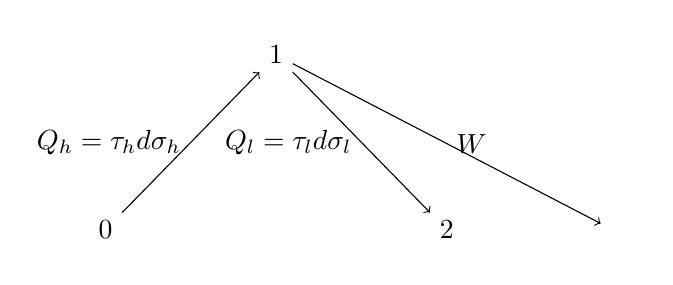
\begin{tikzpicture}
  \matrix (m) [matrix of math nodes, row sep=5em, column sep=5em, minimum width=1em]
  {
 & 1 &   & \\
0 &  & 2 & \phantom{x}\\  };
  \path[->]
  (m-2-1) edge node [left] {$Q_h = \tau_h d\sigma_h$} (m-1-2)
  (m-1-2) edge node [left] {$Q_l = \tau_l d\sigma_l$} (m-2-3)
  (m-1-2) edge node [right] {$W$} (m-2-4)
;
\end{tikzpicture} \quad \quad \, \begin{tikzpicture}
  \matrix (m) [matrix of math nodes, row sep=5em, column sep=5em, minimum width=1em]
  {
 & (\sigma_1,V_0) &   & \\
(\sigma_0,V_0) &  & (\sigma_2,V_1) & \\  };
  \path[|->]
  (m-2-1) edge node [left] {$Q_h = \tau_h d\sigma_h$} (m-1-2)
  (m-1-2) edge node [right] {$Q_l = \tau_l d\sigma_l$} (m-2-3)
;
\end{tikzpicture}
\[
\begin{gathered}
W+ Q_l = Q_h \text{ or } W=Q_h - Q_l \\
W = Q_h - Q_l \leq \frac{ \tau_h - \tau_l}{ \tau_h} Q_h = \eta_C Q_h
\end{gathered} \quad \quad \quad \, 
\begin{gathered}
  \sigma_l = \sigma_h \text{ so } \frac{ Q_h}{\tau_h } = \frac{ Q_l }{ \tau_l}
\end{gathered}
\]

\textbf{Carnot efficiency} $\eta_C \equiv \frac{\tau_h - \tau_l}{\tau_h}$ is the ratio of the work generated to the heat added, in the reversible process.  



\subsection*{Carnot cycle}

\quad \quad \, 

\begin{tikzpicture}
  \matrix (m) [matrix of math nodes, row sep=5em, column sep=5em, minimum width=1em]
  {
3 & 2  \\
4 & 1 \\  };
  \path[->]
  (m-2-2) edge node [right] {$-W_1^2 = Q_h$} (m-1-2)
  (m-1-2) edge node [above] {$W_2^3$} (m-1-1)
  (m-1-1) edge node [left] {$W_3^4$} (m-2-1)
  (m-2-1) edge node [below] {$W_4^1$} (m-2-2)
;
\end{tikzpicture} \quad \quad 
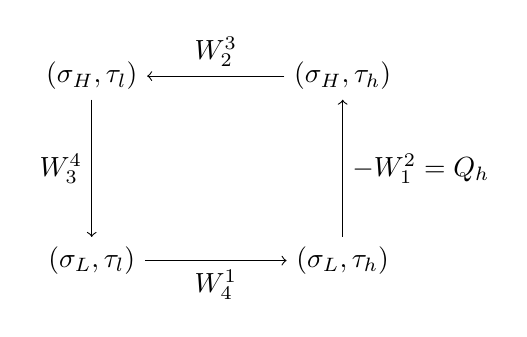
\begin{tikzpicture}
  \matrix (m) [matrix of math nodes, row sep=5em, column sep=5em, minimum width=1em]
  {
(\sigma_H,\tau_l) & (\sigma_H, \tau_h) \\
(\sigma_L, \tau_l) & (\sigma_L,\tau_h) 
\\  };
  \path[->]
  (m-2-2) edge node [right] {$-W_1^2 = Q_h$} (m-1-2)
  (m-1-2) edge node [above] {$W_2^3$} (m-1-1)
  (m-1-1) edge node [left] {$W_3^4$} (m-2-1)
  (m-2-1) edge node [below] {$W_4^1$} (m-2-2)
;
\end{tikzpicture}

The total work is as such: $\oint dU =0$ for 2 reasons: mathematically, the integration of an exact 1-form around a closed curve is $0$, and physically, we return the system back to its original state, as this is a reversible process.  
\[
\oint dU = 0 = \oint \tau d\sigma - \oint p dV \Longrightarrow -\oint W = \oint \tau d\sigma = \left[ \tau_h(\sigma_H - \sigma_L) + 0 + \tau_l (\sigma_L - \sigma_H) + 0 \right] = (\tau_h - \tau_l)(\sigma_H - \sigma_L)
\]

\subsubsection*{Example: Carnot cycle for an ideal gas}

\quad \quad \, 

\begin{tikzpicture}
  \matrix (m) [matrix of math nodes, row sep=5em, column sep=5em, minimum width=1em]
  {
3 & 2  \\
4 & 1 \\  };
  \path[->]
  (m-2-2) edge node [right] {$-W_1^2 = Q_h$} (m-1-2)
  (m-1-2) edge node [above] {$W_2^3$} (m-1-1)
  (m-1-1) edge node [left] {$W_3^4=-Q_l$} (m-2-1)
  (m-2-1) edge node [below] {$W_4^1$} (m-2-2)
;
\end{tikzpicture} \quad \quad 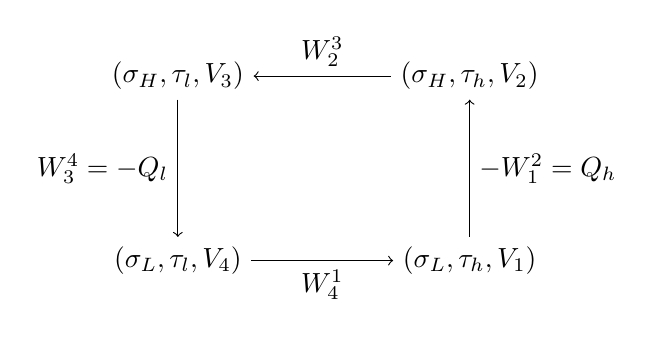
\begin{tikzpicture}
  \matrix (m) [matrix of math nodes, row sep=5em, column sep=5em, minimum width=1em]
  {
(\sigma_H,\tau_l,V_3) & (\sigma_H,\tau_h,V_2)  \\
(\sigma_L,\tau_l,V_4) & (\sigma_L,\tau_h,V_1)   \\  };
  \path[->]
  (m-2-2) edge node [right] {$-W_1^2 = Q_h$} (m-1-2)
  (m-1-2) edge node [above] {$W_2^3$} (m-1-1)
  (m-1-1) edge node [left] {$W_3^4=-Q_l$} (m-2-1)
  (m-2-1) edge node [below] {$W_4^1$} (m-2-2)
;
\end{tikzpicture}

with

\[
\begin{aligned}
\text{isothermal expansion }  & Q_h =- W_1^2 = \int_1^2 p dV = N\tau_h \ln{ \left( \frac{V_2}{ V_1} \right) } \\
\text{adiabatic expansion }  & W_2^3 = - \int_2^3 dU = U(\tau_h) - U(\tau_l) = C_V(\tau_h-\tau_l) \\
\text{isothermal compression } & -Q_l = W_3^4 = \int_3^4-pdV = N\tau_l \ln{ \frac{V_3}{V_4}} \\
\text{adiabatic compression } & W_4^1 = C_V (\tau_h - \tau_l)
\end{aligned} \quad \quad \quad \, \begin{aligned} 
& \quad \\
  & \tau_l V_3^{\gamma-1} = \tau_h V_2^{\gamma-1} \text{ or } \frac{V_3}{V_2}  = \left( \frac{ \tau_h}{ \tau_l} \right)^{\frac{1}{\gamma-1} } \\
  & \quad \\
  & \frac{V_4}{V_1} = (\frac{\tau_h}{ \tau_l } )^{ \frac{1}{\gamma-1 } }
\end{aligned}
\]

EY : 20150911 I don't have a good reason why $C_V$ which is defined for constant $V$, that $C_V \equiv \left( \frac{ \partial U}{ \partial \tau} \right)_V$, can be used in the isentropic (i.e. adiabatic) expansion from $2\to 3$.  

The total work done is 
\[
W = N(\tau_h - \tau_l) \ln{ \left( \frac{V_2}{V_1} \right)}
\]

\subsubsection*{Energy Conversion and the Second Law of Thermodynamics}

\quad \quad \, 

\begin{tikzpicture}
  \matrix (m) [matrix of math nodes, row sep=5em, column sep=5em, minimum width=4em]
  {
1_1 &     & &     & 1_2 & \phantom{x}\\
    & 0_1 & & 0_2 &     &  \\
    &     & &     &     &
\\ };
  \path[->]
  (m-1-1) edge node [auto] {$Q_h$} (m-2-2) 
          edge node [auto] {$Q_h$} (m-2-4)
  (m-1-5) edge node [above] {$W_1 = \eta_1 Q_h$} (m-1-1)
          edge node [above] {$W_{\text{out}} = \eta_2 Q_h - \eta_1 Q_h$} (m-1-6) 
          edge node [right] {$Q_{l_2}$} (m-2-4)
          edge[bend left=120] node [below] {$Q_{l_2}=(1-\eta_2)Q_h$} (m-2-2)
  (m-2-4) edge[transform canvas={xshift=-3mm}] node [auto] {$Q_h$} (m-1-5)
  (m-2-2) edge[transform canvas={xshift=-3mm}] node [left] {$Q_{l_1}=(1-\eta_1)Q_h$} (m-1-1)        
  (m-3-1) edge node [left] {$Q(\text{in})=(\eta_2-\eta_1)Q_h$} (m-2-2)        
;
\end{tikzpicture}

$Q_{l_2}$ waste heat

\begin{tikzpicture}
  \matrix (m) [matrix of math nodes, row sep=4em, column sep=4em, minimum width=2em]
  {
1_1 &     & &     & 1_2 & \phantom{x}\\
    & 0_1 & & 0_2 &     &  \\
    &     & &     &     &
\\ };
  \path[->]
  (m-1-1) edge node [auto] {$$} (m-2-2) 
          edge node [auto] {$Q_h$} (m-2-4)
  (m-1-5) edge node [above] {$W_1$} (m-1-1)
          edge node [above] {$W_{\text{out}}$} (m-1-6) 
          edge node [auto] {$$} (m-2-4)
          edge[bend left=120] node [below] {$Q_{l_2}$} (m-2-2)
  (m-2-4) edge[transform canvas={xshift=-3mm}] node [auto] {$$} (m-1-5)
  (m-2-2) edge[transform canvas={xshift=-3mm}] node [auto] {$$} (m-1-1)        
  (m-3-1) edge node [left] {$Q(\text{in})$} (m-2-2)        
;
\end{tikzpicture}

So with $Q(\text{in})$ heat in, $W_{\text{out}}$ net work can be done.  But that's a decrease in overall entropy.  This violates the law of increasing entropy.  

Define $H = U + pV$.  $H \in C^{\infty}(\Sigma)$, where $\Sigma$ is the manifold of equilibrium (and non-equilibrium) states of the system.  

\subsubsection*{Path Dependence of Heat and Work}

Mathematically, $Q$ and $W$ are not necessarily \emph{exact} 1-forms.  So they are path-dependent.

EY : 20150911 That $Q$, $W$ are not necessarily exact 1-forms would imply that $\Sigma$ has some nontrivial, interesting \emph{topological} features.  

\subsection*{Heat and Work at Constant Temperature or Constant Pressure}

\subsubsection*{isothermal work}

\[
\begin{gathered}
  dU = W + Q = W + \tau d\sigma \\ 
  F = U-\tau \sigma \\ 
  dF = dU - \tau d\sigma - \sigma d\tau = W -\sigma d\tau
\end{gathered}
\]
If $d\tau =0$, on an isothermal curve, \\
$dF = W$, $W$ becomes an exact 1-form, with potential function $F$, the Helmholtz free energy.

\subsubsection*{isobaric heat and work}

e.g. boiling of liquid.  When liquid boils under atmospheric pressure, vapor pressure displacing atmospheric odes work against atmospheric pressure.  isobaric process.

Consider this change of volume: \\
$dx = \frac{dV}{A}$.  Now \\
$p_{\text{eq}} = $ vapor pressure.  \\

$F = p_{\text{eq}}A = p_{\text{atm}}A$ (force equilibrium)

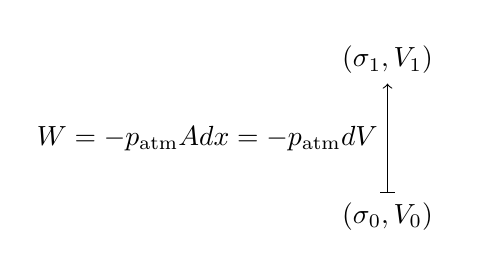
\begin{tikzpicture}
  \matrix (m) [matrix of math nodes, row sep=4em, column sep=4em, minimum width=2em]
  {
(\sigma_1, V_1) \\ 
    (\sigma_0, V_0)
\\ };
  \path[|->]
  (m-2-1) edge node [auto] {$W = -p_{\text{atm}}A dx = -p_{\text{atm}}dV$} (m-1-1) 
;
\end{tikzpicture}

$W = -p_{\text{atm}}dV \equiv - pdV = -d(pV)$ is part of total work done on system.  \\

If $-d(pV) >0$, work provided by environment and is ``free''.  \\
If $-d(pV)<0$, work delivered to environment and not extractable from system for other purposes.  \\
\[
W + d(pV) = dU- Q + d(pV) = dH-Q
\]

Recall that for enthalpy $H = U+pV$, 
\[
dH = dU + Vdp + pdV = dU - W + Vdp = \tau d\sigma + Vdp 
\]
$\sigma, p$ are natural coordinates of $H$.  

\[
dH - Q = W + d(pV)
\]
An isobaric curve s.t. $dp=0$, \\
$dH = Q + W + d(pV)$ \\
so \\
$Q+W$ is an exact 1-form of $H-pV \Longrightarrow d(H-pV) = W+Q$.  

2 classes of constant pressure processes:
\begin{enumerate}
\item[(a)] \[
\begin{aligned} 
  & W + d(pV) = 0 \\
  & dH = Q \end{aligned}
\]
e.g. liquid evaporation from open vessel, because no effective work is done.  \\
heat of evaporation is enthalpy difference between vapor phase and liquid phase
\item[(b)] constant temperature and constant pressure.  
\[
\begin{aligned}
&  G = F + pV = U-\tau \sigma + pV \\ 
& dG = dF + V dp + p dV = dU - \tau d\sigma - \sigma d\tau + V dp  + p dV = V dp- \sigma d\tau \\
&  dG = W - \sigma d\tau + d(pV) = W + d(pV) - \sigma d\tau
\end{aligned}
\]
with natural variables are $p,\tau$ 

at constant temperature, $W + d(pV)$ is exact 1-form, $dG$  
\end{enumerate}

\subsection*{Problems}

\solutionhead{1} \textbf{Heat pump.} \begin{itemize}
\item[(a)] For a heat pump, \\
input: $\sigma_h = \frac{Q_h}{\tau_h}$ \\
output: $\sigma_l = \frac{ Q_l}{\tau_l}$

Reversible condition: $\sigma_h = \sigma_l = \frac{Q_h}{\tau_h} =  \frac{Q_l}{ \tau_l}$  so that $Q_h = \frac{\tau_h}{\tau_l} Q_l$.  

$Q_h - Q_l = Q_h - \frac{ \tau_l}{\tau_h} Q_h = \frac{\tau_h - \tau_l }{\tau_h } Q_h $ net heat inputted to pump heat.  

Thus,
\[
\frac{W}{Q_h} = \eta_c = \frac{ \tau_h - \tau_l }{\tau_h}
\]
If heat pump is not reversible, $\sigma_h > \sigma_l$, so that $\frac{Q_h}{\tau_h } > \frac{ Q_l}{\tau_l}$ or $\frac{ \tau_l }{ \tau_h } Q_h > Q_l$,
\[
\frac{W}{Q_h} = \frac{Q_h - Q_l }{Q_h } < \frac{Q_h - \frac{\tau_l}{\tau_h} Q_h }{ Q_h } = \eta_{c,\, ideal}
\]
\item[(b)] $Q_h = $ electricity consumed by reversible heat pump.  

Carnot engine: $W = (\tau_{hh} - \tau_l)(\sigma_{hh} - \sigma_l)$, with $\sigma_{hh} = \frac{Q_{hh}}{\tau_{hh}}$, and $\sigma_l = \frac{Q_l}{\tau_l}$

Condition that electricity consumed by reversible heat pump:
\[
W = (\tau_{hh} - \tau_l) \left( \frac{ Q_{hh} }{\tau_{hh}} - \frac{Q_l}{ \tau_l } \right) = Q_h 
\]
Note we let $\sigma_l = \frac{Q_l}{\tau_l}$ since both heat pump andCarnot engine are reversible.  
\[
\begin{gathered}
 \Longrightarrow  \left( \frac{ Q_{hh}}{\tau_{hh}} - \frac{Q_h}{\tau_h} \right) = \frac{Q_h}{ \tau_{hh} - \tau_l}  \Longrightarrow   \frac{ Q_{hh}}{\tau_{hh}} = Q_h \left( \frac{1}{ \tau_{hh} - \tau_l } + \frac{1}{\tau_h} \right) \Longrightarrow \boxed{ \frac{ Q_{hh}}{ Q_h}  = \frac{ \tau_{hh} (\tau_h + \tau_{hh} - \tau_l )}{ \tau_h ( \tau_{hh} - \tau_l ) } }
\end{gathered}
\]
For $T_{hh} = 600 \, K$, $T_h = 300 \, K$, $T_l = 270 \, K$, 
\[
\frac{Q_{hh}}{Q_h} = \frac{ 600 (300 + 600 - 270) }{ 300 (600 - 270) } = 3.82
\]

\item[(c)] See Figure (\ref{Fi:Problem08.1(c)}).  \begin{figure}
\scalebox{.50}{\includegraphics{Kittel_Kroemer_Thermal_Physics_01_01.png}}\caption{Problem 8.1(c)}\label{Fi:Problem08.1(c)}
\end{figure}
\end{itemize}











\solutionhead{2} \textbf{Absorption refrigerator}.  
\begin{itemize}
\item[(a)] See Figure (\ref{Fi:Problem08.2(a)}).  \begin{figure}
\scalebox{.50}{\includegraphics{Kittel_Kroemer_Thermal_Physics_01_02.png}}\caption{Problem 8.2(a)}\label{Fi:Problem08.2(a)}
\end{figure}
\item[(b)] Given $\tau_{hh} > \tau_h$, \\
  by energy conservation: $Q_{hh} + Q_l - Q_h = 0$ \\
  reversible refrigerator: $\sigma_{hh} + \sigma_l - \sigma_h = 0$,
\[
\Longrightarrow \frac{Q_{hh} }{ \tau_{hh} } + \frac{ Q_l }{ \tau_l} - \frac{Q_h}{ \tau_h } = 0 
\]
\[
\frac{Q_{hh}}{\tau_{hh} } + \frac{Q_l}{ \tau_l } = \frac{Q_{hh}+Q_l }{ \tau_h} \text{ or } Q_{hh} \left( \frac{1}{ \tau_{hh}} - \frac{1}{\tau_h} \right) = Q_l \left( \frac{1}{\tau_h } - \frac{1}{ \tau_l } \right)
\]
\[
\frac{Q_l}{ Q_{hh}} = \left( \frac{1}{ \tau_{hh} } - \frac{1}{\tau_h} \right)/ \left( \frac{1}{\tau_h} - \frac{1}{ \tau_l } \right) = \left( \frac{ \tau_h - \tau_{hh}}{ \tau_h \tau_{hh}} \right)/ \left( \frac{\tau_l - \tau_h }{ \tau_h \tau_l } \right) = \boxed{ \left( \frac{\tau_{hh} - \tau_h }{ \tau_h - \tau_l } \right)\left( \frac{\tau_l }{ \tau_{hh} } \right) = \frac{Q_l }{ Q_{hh}} }
\]

Note that $Q_l - Q_h = Q_l - (Q_{hh} + Q_l ) = -Q_{hh}$; we've removed $Q_{hh}$ heat from refrigerator's inside.  
\end{itemize}











\solutionhead{3} \textbf{Photon Carnot engine.} Recall, photons are relativistic: $\epsilon  = pc$.  Recall $ p = \frac{ \hbar }{ i} \nabla$.  $ \Longrightarrow \epsilon_s = pc = \hbar k_s c = \left( \frac{ n_s \pi }{L} \right) \hbar c$.  

Recalling that there are 2 polarization states for a photon in 3-dim. space,
\[
\begin{aligned}
  U & = (2) \left( \frac{1}{8} \right) (4\pi ) \int_0^{\infty} n^2 dn \left( \frac{n \pi }{L} \hbar c \right) e^{ - \frac{ n \pi}{L} \hbar c /\tau } = \frac{\pi^2 \hbar c }{L } \int_0^{\infty} n^3 dn exp{ \left( \frac{- \pi \hbar c}{ L \tau} n \right) } = \\
& = \left( \frac{ \pi^2 \hbar c}{L} \right) \lbrace \left. n^3 exp{ \left( \frac{ - \pi \hbar c}{ L \tau } n \right) } \left( \frac{ L \tau }{ -\pi \hbar c} \right) \right|_0^{\infty} - \int_0^{\infty} 3n^2 exp{ \left( \frac{ - \pi \hbar c}{ L \tau } n \right) } \left( \frac{ L \tau }{ -\pi \hbar c} \right) dn \rbrace = \\
  & = \left( \frac{\pi^2 \hbar c}{L} \right) \lbrace (-1) \left( \frac{ - K \tau}{\pi \hbar c} \right) 3 \int_0^{\infty} n^2 exp{ \left( \frac{ - \pi \hbar c}{ L \tau } n \right) } dn \rbrace = \\
  & = \left( \frac{ \pi^2  \hbar c}{L} \right) \lbrace (-1) \left( \frac{-L \tau}{\pi \hbar c} \right)3 \lbrace \left. n^2 exp{ \left( \frac{ - \pi \hbar c}{ L \tau } n \right) } \left( \frac{ L \tau }{ -\pi \hbar c} \right) \right|_0^{\infty} - \int_0^{\infty} 2n exp{ \left( \frac{ - \pi \hbar c}{ L \tau } n \right) } \left( \frac{ L \tau }{ -\pi \hbar c} \right) dn = 
\end{aligned} 
\]
\[
\begin{aligned} 
 & = \left( \frac{ \pi^2 \hbar c}{L} \right) (-1)^2 \left( \frac{ - L \tau}{ \pi \hbar c } \right)^2 3 (2) \int_0^{\infty} n exp{ \left( \frac{ - \pi \hbar c}{ L \tau } n \right) } \left( \frac{ L \tau }{ -\pi \hbar c} \right) dn = \\
  & = \left( \frac{\pi^2 \hbar c}{L} \right)(-1)^3 \left( \frac{ -L \tau}{\pi \hbar c} \right)^3 3(2)(1) \int_0^{\infty } exp{ \left( \frac{ - \pi \hbar c}{ L \tau } n \right) } dn = \left( \frac{\pi^2 \hbar c}{L} \right)(-1)^3 \left( \frac{-L \tau}{\pi \hbar c} \right)^4 3(2)1 \left. \left( \exp{ \left( \frac{-\pi \hbar c}{ L \tau} n \right) } \right) \right|_0^{\infty} = \\
  & = 6 \left( \frac{ L }{ \pi^2 \hbar c } \right)^3 \tau^4 = \boxed{ 6 \frac{ V}{ (\pi^2 \hbar c )^3} \tau^4  = U }
\end{aligned}
\]

To get the entropy, \emph{recall}, $\left( \frac{ \partial \sigma}{ \partial U} \right)_V = \frac{1}{\tau}$, and using this is usually the \emph{most direct way to obtain entropy}.
\[
\Longrightarrow d\sigma = \int \frac{dU}{ \tau} = \int \frac{6V}{ (\pi^2 \hbar^2 c)^3 } 4 \tau^3 \frac{d\tau}{ \tau} = \frac{6V}{ (\pi^2 \hbar^2 c)^3} \frac{1}{3} \tau^3 \Longrightarrow \boxed{ \sigma(\tau) = \frac{ 8 V \tau^3 }{ (\pi^2 \hbar^2 c)^3 } }
\]  

Consider  \\
Isothermal expansion: Helmholtz free energy $F$ is needed.  
\[
F = U - \tau \sigma = \frac{ 6V}{ (\pi^2 \hbar^2 c)^3 } \tau^4 - \tau \frac{ 8 V \tau^3 }{ (\pi^2 \hbar^2 c)^3 } = -\frac{ 2 V \tau^4 }{ (\pi^2 \hbar^2 c)^3 }
\]
Then 
\[
\begin{gathered}
p  = -\left( \frac{ \partial F}{ \partial V} \right)_{ \tau, \, N} = \frac{2 \tau^4}{ (\pi^2 \hbar^2 c)^3 } \\
W_{12} = p (V_2 - V_1) = \frac{ 2 \tau_h^4 }{ (\pi^2 \hbar^2 c)^3 } (V_2 - V_1)
\end{gathered} \quad \quad \, 
\begin{gathered}
\sigma_{12} = \frac{ 8 \tau_h^3 }{ (\pi^2 \hbar^2 c)^3 }(V_2 - V_1)  \\
\Delta Q_{12} = \frac{ \tau} \Delta \sigma = \frac{ 8 \tau_h^4}{ (\pi^2 \hbar^2 c)^3} (V_2 - V_1)
\end{gathered}
\]

Isentropic expansion: $\Longrightarrow V_2 \tau_h^3 = V_3 \tau_l^3$ or $V_3 = V_2 \left( \frac{ \tau_h}{\tau_l }\right)^3$.  

So for this isentropic process, $V_2 \tau_h^3 = V\tau^3$, 
\[
U = \frac{6V}{ (\pi^2 \hbar^2 c)^3} \left( \frac{V_2 \tau_h^3}{V}\right)^{4/3} = \frac{ 6(V_2 \tau_h^3 )^{4/3} }{ (\pi^2 \hbar^2 c)^3} V^{-1/3}
\]
\[
p = \frac{- \partial U}{ \partial V} = - \frac{ 6 (V_2 \tau_h^3 )^{4/3} }{ (\pi^2 \hbar^2 c)^3} \left( \frac{-1}{3} V^{-4/3} \right) = \frac{ 2 ( V_2 \tau_h^3 )^{4/3} }{ (\pi^2 \hbar^2 c )^3 } V^{-4/3}
\]
\[
\begin{aligned}
W_{23} & = \int p dV = \int \frac{ 2 (V_2 \tau_h^3 )^{4/3}}{ (\pi^2 \hbar^2 c)^3 } V^{-4/3} dV = \left. \frac{ 2 (V_2 \tau_h^3 )^{4/3} }{ (\pi^2 \hbar^2 c)^3}  ( -3V^{-1/3} ) \right|_{V_2}^{V_3} = \frac{ -6 (V_2 \tau_h^3 )^{4/3} }{ (\pi^2 \hbar^2 c)^3 } \left( \frac{1}{V_3^{1/3}} - \frac{1}{ V_2^{1/3} } \right) = \\
& = \frac{ 6 V_2 \tau_h^4}{ (\pi^2 \hbar^2 c)^3} \left( 1 - \frac{\tau_l }{\tau_h} \right)
\end{aligned}
\]

Isothermal compression: $W_{34} = \frac{ 2\tau_l^4}{ (\pi^2 \hbar^2 c)^3 } (V_4 - V_3) = \frac{ 2 \tau_h^3 \tau_l }{ (\pi^2 \hbar^2 c)^3 } (V_1 - V_2)$.  \\  $\sigma_{34} = \frac{8 \tau_l^3}{ (\pi^2 \hbar c)^3} (V_4 - V_3) = \frac{ 8 \tau_h^3 }{(\pi^2 \hbar c)^3} (V_1 -V_2 )$.  

Isentropic compressiong: $V_4 \tau_l^3 = V_1 \tau_h^3$ or $V_4 = V_1 \left( \frac{\tau_h}{\tau_l} \right)^3$.  
\[
W_{41} = \frac{ 6 (V_4 \tau_l^3 )^{4/3} }{ (\pi^2 \hbar^2 c)^3 } \left( \frac{1}{V_4^{1/3}} - \frac{1}{V_1^{1/3}} \right) = \frac{ -6 V_1 \tau_h^4}{ (\pi^2 \hbar^2 c)^3} \left( 1 - \frac{ \tau_l }{\tau_h } \right)
\]

\[
\Delta W = \frac{ 2 \tau_h^4}{ (\pi^2 \hbar^2 c)^3} (V_2 - V_1) + \frac{ 6 V_2 \tau_h^4}{ (\pi^2 \hbar^2 c)^3} \left( 1 - \frac{\tau_l}{\tau_h} \right) + \frac{ 2 \tau_h^3 \tau_l }{ (\pi^2 \hbar^2 c)^3} (V_1 - V_2) + \frac{ -6 V_1 \tau_h^4}{ (\pi^2 \hbar^2 c)^3} \left( 1 - \frac{\tau_l }{\tau_h} \right) = \frac{ 8 \tau_h^4 ( V_2 -V_1)}{ (\pi^2 \hbar^2 c)^3} \left( 1 - \frac{\tau_l }{\tau_h} \right)
\]
\[
Q_h = \frac{ 8 \tau_h^4 (V_2 - V_1) }{ (\pi^2 \hbar c)^3} \Longrightarrow \boxed{ \frac{ \Delta W}{ Q_h } = 1 - \frac{\tau_l}{\tau_h} }
\]












\solutionhead{4} \textbf{Heat engine-refrigerator cascade}.  Consider the heat engine as a Carnot cycle.  
\[
W + W_r = (\tau_h - \tau_l) \sigma_h
\]
where $W_r = $ work consumed by refrigerator.  
\[
\sigma_h = \frac{Q_h}{\tau_h} = \frac{Q_l}{\tau_l} = \sigma_l
\]
This must be true for \emph{any} heat engine undergoing Carnot cycle; furthermore, we can say it's the most efficient heat engine possible.  

reversible refrigerator: $Q_L + W_r = Q_H$, (by $E$-consv.) \\
$\sigma_L = \sigma_H = \frac{Q_L}{\tau_L} = \frac{Q_H}{\tau_H}$, (by reversible condition)

Note, $Q_l$ is energy transfer from heat engine to $\tau_l$ reservoir.  $Q_L$ is energy transfer from $\tau_l$ reservoir to refrigerator.  $Q_L \geq Q_l$, otherwise, no cooling, no thermal energy extracted from $\tau_l$ resevoir to lower its temperature.  $Q_L = Q_l$ at equilibrium; no further cooling, $\tau_r$ reached.  

Note that $\tau_l$ is given as the environmental temperature.  Assume refrigerator throws out $Q_H$ heat into the environment.  $\to \tau_H = \tau_l$.  Since $Q_L$ heat inputed into refrigerator from a $\tau_l$ reservoir now lowered to $\tau_r$, $\tau_l \to \tau_r$.  
\[
W_r = \frac{\tau_l }{ \tau_r } Q_L -  Q_L = \left( \frac{ \tau_l }{ \tau_r } - 1 \right) Q_L
\]
since for a reversible refrigerator, $\sigma_L = \sigma_H = \frac{ Q_L}{\tau_L} = \frac{Q_H}{\tau_H}$.  

\[
\Longrightarrow \frac{W}{Q_h} = \left( 1 - \frac{\tau_r }{\tau_h} \right) - \left( \frac{ \tau_l }{ \tau_r} - 1 \right) \frac{Q_L}{Q_h} = \left( 1 - \frac{\tau_r }{ \tau_h } \right) - \left( \frac{\tau_l }{ \tau_r } -1 \right) \left( \frac{\tau_r }{\tau_h } \right) = \boxed{ 1 - \frac{\tau_l }{\tau_h} }
\]
Combinations of reversible systems $=$ reversible system.  








\solutionhead{5} \textbf{Thermal pollution}.  Given $\begin{aligned} T_l & = 20^{\circ} \, C \\ T_h & = 500^{\circ} \, C \end{aligned}$.  Consider a Carnot cycle.  
\[
W = (\tau_h - \tau_l )\sigma_l = (\tau_h - \tau_l) \frac{Q_l}{\tau_l} = \left( \frac{\tau_h}{\tau_l} - 1 \right) Q_l = \left( \frac{500}{20} - 1 \right) 1500 \, MW = \boxed{ 36000 MW }
\]

If improvements in hot-steam technology would permit raising $T_h$ by $100^{\circ} \, C$, 
\[
W = \left( \frac{600}{20}  -1 \right) 1500 \, MW = (29)(1500 \, MW)  = 43500 \, MW 
\]
There was a $17.2 \, \%$ increase in output.  





\solutionhead{6} \textbf{Room air conditioner}.  \begin{itemize}
\item[(a)] \[
\begin{gathered}
  W = (\tau_h - \tau_l) \frac{Q_l}{\tau_l} = \left( \frac{\tau_h }{\tau_l }- 1 \right)Q_ l \\
  P = \left( \frac{\tau_h}{\tau_l} - 1 \right) \frac{dQ_l}{dt} = \left( \frac{\tau_h }{\tau_l }-1 \right) A (\tau_h - \tau_l ) \Longrightarrow \frac{P}{A} \tau_l = (\tau_h - \tau_l )(\tau_h - \tau_l) = \tau_h^2 - 2\tau_h \tau_l + \tau_l^2
\end{gathered}
\]

\[
\Longrightarrow \tau_l^2 - 2\tau_h \tau_l  - \frac{P}{A} \tau_l + \tau_h^2 = 0 
\]
\[
\boxed{ \tau_l = \tau_h + \frac{P}{2A} - \sqrt{ (\tau_h + \frac{P}{2A} )^2 - \tau_h^2 } }
\]
\item[(b)] For $T_l = 17^{\circ} \, C = 290 \, K$, $T_h = 310 \, K$, 
\[
A = \frac{P\tau_l }{ (\tau_h - \tau_l)^2 } = \frac{ ( 2 \, kW )(290 \, K) }{ (310 - 290)^2 } = \frac{580 \times 10^3 \, W }{ 400 \, K } = \boxed{ 1450 \, \frac{W}{K} }
\]
\end{itemize}






\solutionhead{7} \textbf{Light bulb in a refrigerator}

Carnot refrigerator draws 100 W.  For any Carnot cycle,
\[
W = (\tau_h - \tau_l) \frac{Q_l}{\tau_l} = \left( \frac{\tau_h }{\tau_l } - 1 \right) Q_l = \left( 1 - \frac{\tau_l }{\tau_h} \right) Q_h 
\]

Carnot refrigerator expels $Q_h$ thermal energy to hot $\tau_h$ environment and \emph{inputs} $Q_l$ thermal energy from $\tau_l$ reservoir.  
\[
Q_l + W = Q_h
\]

Work $W$ must be drawn by Carnot refrigerator to do work.  Suppose Carnot cycle part of the refrigerator must input in heat from light bulb to cool down its inside, i.e. consider Carnot refrigerator in \emph{equilibrium with light bulb, now inputting in heat from light bulb} $Q_{ext}$, and drawing in work to expend out $Q_h$ thermal energy into the environment.  
\[
\Longrightarrow \boxed{ Q_{ext} = Q_l }
\]
$\dot{W} = \dot{Q}_l$ in this case, so 
\[
\left( \frac{\tau_h}{\tau_l } - 1 \right) Q_l - Q_l = 0 \text{ or } \left( \frac{\tau_h }{\tau_l } - 2 \right) Q_l = 0 
\]
\[
\Longrightarrow \boxed{ \tau_l = \frac{\tau_h}{2} } = \frac{300 \, K}{2} = 150 \, K
\]











\solutionhead{8} \textbf{Geothermal energy}.  

Given $\Delta Q_h = -MC dT_h$, \\
$T_l$ lower reservoir temperature stays constant.   $\tau_h$ decreasing, $d\tau_h < 0$.  

\[
\Delta W = (\tau_h - \tau_l ) \frac{\Delta Q_h}{\tau_h} = \left( 1 - \frac{\tau_l}{\tau_h} \right) (-MC) \frac{d\tau_h }{k_B} 
\]
\[
\Longrightarrow W = - \left( \frac{MC}{k_B} \right) \left. ( \tau_h - \tau_l \ln{ \tau_h } ) \right|_{\tau_i}^{\tau_f} = - \left( \frac{MC}{k_B} \right) \left( \tau_l \ln{ \left( \frac{\tau_i }{\tau_f} \right)} - (\tau_i - \tau_f ) \right) 
\]

For $M = 10^{17} \, g$, $C = 1 \, J/g\cdot K$, $T_l = 20^{\circ} \, C = 293 \, K$, $T_i = 600^{\circ} \, C = 873 \, K$, $T_f = 110^{\circ} \, C = 383 \, K$
\[
W = 2.486 \times 10^{19} \, J
\]
Note that $10^{14} \, kWh = 10^{17} \, \frac{J}{s} \cdot h \left( \frac{3600 \, sec}{1 \, h }\right) = 3.6\times 10^{20} \, J$.  






\solutionhead{9} \textbf{Cooling of nonmetallic solid to $T=0$}.  Recall that $C = aT^3 = \left( \frac{ \partial U}{ \partial T} \right)_V$.  Then $dQ_l = aT_l^3 dT_l$.  Now $d\tau_l <0$ since $\tau_l$ decreasing.  

For the refrigerator: $Q_l + W = Q_h$.  

\[
\begin{aligned}
  dW & = (\tau_h - \tau_l ) \frac{ Q_l}{\tau_l } = - \left( \frac{\tau_h}{\tau_l } - 1 \right) (a\tau_l^3 d\tau_l ) \left( \frac{1}{k_B^4} \right) = \frac{ -a}{k_B^4} \left( \frac{ \tau_h }{\tau_l } - 1 \right) \tau_l^3 d\tau_l = \frac{-a}{k_B^4} ( \tau_h \tau_l^2 - \tau_l^3 ) d\tau_l 
\end{aligned}
\]
\[
\begin{aligned}
  W = \left. \frac{-a}{k_B^4} \left( \tau_h \frac{1}{3} \tau_l^3 - \frac{1}{4} \tau_l^4 \right) \right|_{\tau_h}^0 = \boxed{ \frac{a T_h^3}{ 12 k_B } =W }
\end{aligned}
\]
















\section{Gibbs Free Energy and Chemical Reactions}

\solutionhead{1} \textbf{Thermal expansion near absolute zero} \begin{itemize}
\item[(a)] \[
\begin{aligned}
  \left( \frac{ \partial G}{ \partial \tau} \right)_{N, \, p } & = - \sigma \\ 
  \left( \frac{ \partial^2 G}{ \partial p \partial \tau} \right)_{\tau}  & = - \left( \frac{ \partial \sigma}{ \partial p } \right)_{\tau}
\end{aligned} \quad \, \begin{aligned} \left( \frac{ \partial G }{ \partial p } \right)_{\tau} & = V \\ \left( \frac{ \partial^2 G}{ \partial \tau \partial p } \right)_p  & =\left( \frac{ \partial V}{ \partial \tau} \right)_p  \end{aligned} \quad \Longrightarrow \boxed{ \left( \frac{ \partial V}{ \partial \tau} \right)_p = -\left( \frac{ \partial \sigma }{ \partial p } \right)_{\tau} }
\]
\[
\begin{aligned}
  \left( \frac{ \partial G}{ \partial N} \right)_{ p } & =  \mu \\ 
  \left( \frac{ \partial^2 G}{ \partial p \partial N} \right)_{N}  & =  \left( \frac{ \partial \mu}{ \partial p } \right)_{N}
\end{aligned} \quad \, \begin{aligned} \left( \frac{ \partial G }{ \partial p } \right)_{\tau} & = V \\ \left( \frac{ \partial^2 G}{ \partial N \partial p } \right)_p  & =\left( \frac{ \partial V}{ \partial N} \right)_p  \end{aligned} \quad \Longrightarrow \boxed{ \left( \frac{ \partial V}{ \partial N} \right)_p = \left( \frac{ \partial \mu }{ \partial p } \right)_{N} }
\]
\[
\begin{aligned}
  \left( \frac{ \partial^2 G}{ \partial \tau \partial N} \right)_{N}  & =  \left( \frac{ \partial \mu}{ \partial \tau } \right)_{N}
\end{aligned} \quad \, \begin{aligned} 
\left( \frac{ \partial^2 G}{ \partial N \partial \tau } \right)_\tau  & = - \left( \frac{ \partial \sigma}{ \partial N} \right)_{\tau}  \end{aligned} \quad \Longrightarrow \boxed{ \left( \frac{ \partial \mu}{ \partial \tau } \right)_N = -\left( \frac{ \partial \sigma }{ \partial N } \right)_{\tau} }
\]
\item[(b)] $\alpha = \frac{1}{V} \left( \frac{ \partial V}{ \partial \tau} \right)_p = \frac{-1}{V} \left( \frac{ \partial \sigma }{ \partial p } \right)_{\tau} = 0$ as $\tau \to 0$ since $\sigma \to $ constant as $\tau \to 0$ by third law of thermodynamics.  
\end{itemize}

\solutionhead{2} \textbf{Thermal ionization of hydrogen}.  
\begin{itemize}
\item[(a)] Given $e + H^+ \rightleftarrows H$, note that $e + H^+ - H =0$.  Recall
\[
\frac{ [e][H^+] }{ [H] } = K(\tau) = \prod_j n_{Q_j}^{\nu_j} \exp{ [ -\nu_j F_j(int) /\tau ] }
\]
where $n_Q = \left( \frac{ M \tau}{2\pi \hbar^2 } \right)^{3/2} V$.  

For dissocation of $H$ into $e^- + H^+$ choose zero of internal energy of each composite particle (here $H$) to concide with energy of dissociated particles (here $H^+$, $e^-$) at rest; place energy of ground state of composite particle $H$ at $-I$, $I$ is energy required in reaction to dissociate composite particle into its constituents and is taken to be positive, i.e. the ionization energy.  

\[
K(\tau) = (n_{e^-})^1 \exp{ [- F_{int}(e^-)/\tau ]} \cdot (n_{H^+} )^1 \exp{ [ -F_{int}(H^+)/ \tau ] } (n_{H})^{-1} \exp{ (- (-1) (F_{int}(H)/\tau) )}
\]
Note that $n_{H^+} \simeq n_{H}$.  Let $n_{e^-} = n_Q$.  \emph{Importantly}, note
\[
\boxed{ F_{int}(e^-) + F_{int}(H^+) - F_{int}(H) = I }
\]
$F_{int}(H)$ is at a lower free energy than $e^-$ and $H^+$.  
\[
\Longrightarrow K(\tau) = n_Q e^{-I/\tau} \Longrightarrow \boxed{ \frac{ [e][H^+] }{ [H] } = n_Qe^{-I/\tau}  }
\]

\item[(b)] By charge conservation, $[e] = [H^+]$, so that 
\[
[e] = [H]^{1/2} n_Q^{1/2} \exp{ (-I/2\tau)}
\]
Given $[H] \simeq 10^{23} \, cm^{-3}$, $m_e = 0.511 \, MeV/c^2$, $T = 5000 \, K$, $I = 13.6 \, eV$ ionization energy,
\[
[e] = (10^{23} \, cm^{-3})^{1/2} ( 2.92 \times 10^{10} 1/cm^{3/2})^{1/2} \exp{ ( - 13.6 \, eV / 2 k_B 5000 \, K) } =  1.3 \times 10^{15} \, cm^{-3}
\]

\emph{Note that $H(exc)$ and $H$ are just two different states of atomic hydrogen.  Their concentrations must therefore be proportional to the probability of occurrence of these states, and the ratio of probabilities is the ratio of the respective Boltzmann}
\[
\frac{ [H(exc) ] }{[H] } = \frac{p(H(exc) )}{ p(H) }
\]

\emph{If $\epsilon_{H(exc)}$ is the internal energy of the first excited state and $\epsilon_H$ is the internal energy of the ground state of atomic hydrogen, we are given that $\epsilon_{H(exc)} - \epsilon_H = \frac{3}{4} I$}.  \textbf{We also need to take into account the fact that the first excited electronic state of hydrogen is 4-fold degenerate i.e. one 2s-orbital and three 2p-orbitals.}\footnote{(from solutions to Homework 8, Ph12c, Caltech, June 6, 2008, by Prabha Mandayam, Heywood Tam)} Therefore,
\[
\frac{ [H(exc)]}{[H]} = \frac{ p(H(exc)) }{ p(H)} = \frac{ 4e^{-\epsilon_{H(exc)}/\tau } }{ e^{-\epsilon_H/\tau} } = 4 e^{-3I/4\tau}
\]   
\[
[H(exc)] = 4[H] e^{-3I/4\tau} = \boxed{ 2.092 \times 10^{13} \, cm^{-3} }
\]
\[
\frac{ [e] }{ [H(exc) ]} = 62
\]

\end{itemize}



\solutionhead{3} \textbf{Ionization of donor impurities in semiconductors}.

Consider a pentavalent impurity (donor), introduced in place of tetravalent silicon atom, acts like a hydrogen atom in free space.  

Then recall, from Problem 3, $e + H^+ \rightleftarrows H$, and so 
\[
\frac{ [e][H^+]}{ [H] } =  n_Q  \exp{ (-I/\tau)}
\]
where $n_Q \equiv \left( \frac{ m\tau }{2\pi \hbar^2 } \right)^{3/2}$ refers to the electron.  

By charge conservation, $[e] = [H^+]$.  

So
\[
[e] = [H]^{1/2} n_Q^{1/2} \exp{ (-I/2\tau)}
\]

Now given $[H] = 10^{17}$ donors per $\text{cm}^3$,  $\tau = 100 \, K$, 
\[
n_Q = \left( \frac{m^* \tau}{2\pi \hbar^2 }\right)^{3/2} = \left( \frac{ 0.3 \cdot 0.511 \, MeV/c^2* 100 \, K \cdot 0.00008617 \, eV/K }{ 2 \pi (4.136 \times 10^{-15} \, eV/s)^2 } \right)^{3/2} = 1263. \text{ donors per $\text{cm}^3$ }
\]
Now $F = \frac{q_1q_2}{r^2}$, 
\[
W = \int -F dr = - \int_{r_0}^{\infty} \frac{q_1 q_2}{r^2} dr = + \left. \left( \frac{q_1 q_2 }{r} \right) \right|_{r_0}^{\infty} = \frac{-q_1 q_2}{r_0}
\]
and so $I = \frac{e^2}{\epsilon r_0} = \frac{1}{\epsilon}(13.6 \, eV)$ where $13.6 \, eV$ is the ionization energy of an electron from a (real) hydrogen atom. 

So
\[
[e]= 2. \times 10^{-18} \, \text{ donors per $\text{cm}^3$ }
\]
















\solutionhead{4} \textbf{Biopolymer growth.}  

Recall that $G(N,p,\tau) = N\mu(p,\tau)$, since $G$ was chosen to be an \emph{extensive} quantity (it scales with size).  For more than one chemical species $G = \sum_j N_j \mu_j$.  \\
$dF = 0$ for equilibrium, for constant $P,\tau$.   \quad \\ 

$\mu_j = $ chemical potential of species $j$, $\mu_j = (\partial G/\partial N_j)_{ \tau, p}$.   \quad \\ 

Given $\sum_i \nu_j A_j$, e.g. $H_2 + Cl_2 = 2HCl$, \\
$dG = (\sum_j \nu_j \mu_j )d\hat{N}$ where $dN_j = \nu_j d\hat{N}$, $dG = 0 \to \sum_j \nu_j \mu_j =0$.   \quad \\ 

Recall the mass action law derivation: assume constituents act as ideal gases; $\mu_j  = \tau(\ln{n_j} - \ln{c_j})$, $n_j$ concentration of species $j$; $c_j \equiv n_{Q_j} Z_j(int)$.  
\[
\sum_j \nu_j\ln{n_j} = \sum_j \nu_j \ln{c_j} \Longrightarrow \sum_j \ln{n_j^{\nu_j}} = \sum_j \ln{c_j^{\nu_j}} = \ln{ \prod_j n_j^{\nu_j} } = \ln{ K(\tau) }
\]
\[
\prod_j n_j^{\nu_j} = K(\tau) \quad \quad \, \text{ mass action law }
\]
\hrulefill

\begin{itemize}
\item[(a)] By mass action law, $\frac{ [\text{ monomer}][N\text{mer}] }{[(N+1)\text{mer}]} = \frac{ [1][N]}{[N+1]} = K_N$.  
\[
\begin{gathered}
  \frac{[1][1]}{[2]} = K_1 \quad \quad \, \frac{ [1]^2}{[2]}\frac{[1][2]}{[3]} = \frac{[1]^3}{[3]} = K_1 K_2 \\ 
  \frac{ [1]^{j+1} }{[j+1]} \frac{ [1][j+1] }{[j+2]} = \prod^j_{l=1} K_l K_{j+1} = \frac{[1]^{j+2}}{[j+2]} = \prod_{l=1}^{j+1} K_l 
\end{gathered} \quad \quad \, \Longrightarrow \boxed{ [N+1]= [1]^{N+1}/K_1 K_2 K_3 \dots K_N }
\]
\item[(b)] Recall that $K(\tau) = \prod_j n_{Q_j}^{\nu_j} \exp{ [ - \nu_j F_j(int)/\tau ]}$  
\[
K_N = \frac{n_Q(N)n_Q(1)}{ n_Q(N+1)} \exp{ \left[ \frac{-F_N}{\tau} - \frac{F_1}{\tau} \right] }\exp{ \left[ \frac{ F_{N+1}}{\tau} \right] } = \frac{ n_Q(N)n_Q(1) }{n_Q(N+1)} \exp{ \left[ \frac{ - (F_N + F_1 - F_{N+1} )}{\tau} \right]}
\]
where $n_Q(N) = \left( \frac{M_N \tau}{2\pi \hbar^2} \right)^{3/2}$ and $M_N$ is the mass of $N$mer molecules, $F_N$ is the free energy of one $N$mer molecule.  
\item[(c)] Assume $N \ll 1$ so $n_Q(N) \simeq n_Q(N+1)$.  Assume $[1] = 10^{20} \, cm^{-3}$.  Assume $\Delta F = F_{N+1} - F_N - F_1 = 0$, meaning zero free energy change in the basic reaction step.  We're given the molecular weight of the monomer to be 200.  

We want $\frac{[N+1]}{[N]}$ at room temperature.  Now $K_N \simeq n_Q(1) = \left( \frac{ M_1 \tau}{2\pi \hbar^2} \right)^{3/2}$.  
\[
\frac{[1][N]}{[N+1]} = n_Q(1) = \left( \frac{M_1 \tau}{2\pi \hbar^2} \right)^{3/2} \text{ or } \frac{ [N+1]}{[N]} = \frac{[1]}{n_Q(1)} = \left( \frac{2\pi \hbar^2}{M_1 \tau} \right)^{3/2} 10^{20} \, cm^{-3}
\]
Note that $\left( \frac{ 2\pi (6.582 \times 10^{-22} \, MeV \cdot s)^2 }{ 200 (938 MeV/c^2)(0.8617 \times 10^{-4} eV/K)(298 \, K) } \left( \frac{ 3\times 10^{10} \, cm/s}{1 \, c} \right)^2 \right)^{3/2} = 0.3627 \times 10^{-27} \, cm$.  

\[
\Longrightarrow \boxed{ \frac{ [N+1]}{[N]} = 3.627 \times 10^{-8} }
\]
\item[(d)] We want the condition
\[
1 < \frac{ [N+1]}{[N]} = \frac{[1]}{n_Q(1)} \exp{ \left( \frac{ -\Delta F}{\tau} \right) } \text{ or } \ln{ \frac{n_Q(1)}{[1]}} < \frac{ - \Delta F}{\tau} 
\]
\[
\Longrightarrow \Delta F < \tau \ln{  \frac{ [1]}{ n_Q(1)} } = \boxed{ - 0.44 \, eV}
\]
\end{itemize}







\section{Phase Transformations}

\subsection*{Vapor Pressure Equation}

\subsubsection*{Derivation of the Coexistence Curve $p$ versus $\tau$}

Suppose $\mu_g(p_0,\tau_0) = \mu_l(p_0,\tau_0)$ and $\mu_g(p_0 + dp, \tau_0 + d\tau) = \mu_l(p_0 + dp, \tau_0 + d\tau)$
\[
\Longrightarrow \mu_g(p_0,\tau_0) + \left( \frac{ \partial \mu_g }{ \partial p} \right)_{\tau} dp + \left( \frac{ \partial \mu_g }{ \partial \tau} \right)_{p} d\tau + \dots = \mu_l(p_0,\tau_0) + \left( \frac{ \partial \mu_l }{ \partial p} \right)_{\tau} dp + \left( \frac{ \partial \mu_l }{ \partial \tau} \right)_{p} d\tau + \dots
\]

\[
\frac{dp}{d\tau} = \frac{ \left( \frac{ \partial \mu_l }{ \partial \tau} \right)_p - \left( \frac{ \partial \mu_g }{ \partial \tau} \right)_p }{ \left( \frac{ \partial \mu_g }{ \partial \tau} \right)_{\tau} - \left( \frac{ \partial \mu_l }{ \partial p} \right)_{\tau} }
\]




$\begin{aligned}
  & v \equiv V/N \\ 
  & s \equiv \sigma /N
\end{aligned}$

\[
\begin{aligned}
  & \frac{1}{N} \left( \frac{ \partial G}{ \partial p } \right)_{N,\tau} = v = \left( \frac{ \partial \mu }{ \partial p } \right)_{\tau} \\ 
  & \frac{1}{N} \left( \frac{ \partial G}{ \partial \tau} \right)_{N,p} = \frac{-\sigma}{N} = -s = \left( \frac{ \partial \mu }{ \partial \tau} \right)_p
\end{aligned}
\]


$s_g-s_l$ related directly to quantity of heat that must be added to system to transfer 1 molecule reversibly from liquid to gas, while temperature constant.  (if heat isn't added to system from outside in the process, temperature will decrease when molecule transferred to gas)
\begin{equation}
  L \equiv \tau(s_g - s_l)
\end{equation}
\textbf{latent heat of vaporization}

\begin{equation}
  \Delta v = v_g - v_l
\end{equation}
change of volume when 1 molecule transferred from liquid to gas

\begin{equation}
  \frac{dp}{d \tau} = \frac{ L }{ \tau \Delta v}
\end{equation}
is the \textbf{ Clausius-Clapeyron equation} or \textbf{vapor pressure equation}.  

Assumptions:
\begin{enumerate}
  \item[(a)] if assume $v_g \gg v_l$, then $\Delta v \cong v_g = V_g/N_g$ at $p=1$ atm (at atmospheric pressure), $v_g/v_l \approx 10^3$
  \item[(b)] ideal gas law $pV_g = N_g \tau \Longrightarrow \Delta v \cong \tau/p$
\end{enumerate}
\[
\frac{dp}{d\tau} = \frac{L}{\tau^2}p \text{ or } \frac{d}{d\tau} \ln{p} = \frac{L}{\tau^2}
\]
$L \equiv $ latent heat per molecule

If latent heat $L$ independent of temperature over temperature range of interest, $L = L_0$ \\
\phantom{\quad \, } $\int \frac{dp}{p} = L_0 \int \frac{d\tau}{\tau^2}$ whence $\ln{p} = -L_0/\tau + \text{const}$ or $p(\tau) = p_0\exp{ (-L_0/\tau)}$



Consider $\frac{L_0}{\tau}$, $L_0$, latent heat of vaporization of \emph{1 molecule}.  

Now compare it with $\frac{L_0}{RT}$, \\
where $R \equiv N_0 k_B \equiv $ gas constant.  

$N_0 = 6.02205 \times 10^{23} \frac{1}{ \text{mol}}$ \\
$k_B = 1.38066 \times 10^{-23} \, J/K$ (usual Boltzmann constant) \\
$R = 8.31441 \, J/K\cdot \text{mol}$ 

So for 
\[
\frac{L_0}{RT} = \frac{L_0}{N_0 k_B T}
\]
Then that implies
\[
\frac{1}{ 1 \text{ particle} } \frac{1}{N_0} = \frac{1}{ 1 \text{ particle } \frac{1}{ \text{ mol }} }
\]
which implies that $L_0$ now is the latent heat of vaporization of a \emph{mole (mol)} of the gas.  



\subsubsection*{Latent heat and enthalpy}

crossing the coexistence curve,
\[
\tau d\sigma = dU + pdV - (\mu_g - \mu_l) dN
\]
if liquid $\to$ gas, $\mu_l > \mu_g$ (or $0 > \mu_g - \mu_l$)

on coexistence curve, $\mu_g = \mu_l$
\[
L = \tau d\sigma(\dot{\gamma}) = dU(\dot{\gamma}) + pdV(\dot{\gamma}) = (dU+ pdV)(\dot{\gamma}) + 0 = (dU + pdV)(\dot{\gamma}) + Vdp(\dot{\gamma}) = dH(\dot{\gamma}) = H_g -H_l
\]
where $dp(\dot{\gamma}) = 0$ since $\gamma$ is a path s.t. pressure $p$ is constant.  

Recall that $\begin{gathered} \quad \\
  H = U + pV \\
  dH = dU+ pdV + Vdp \end{gathered}$.  


$C_p = \tau \left( \frac{ \partial \sigma }{ \partial \tau} \right)_p = \tau\sigma(\tau,p)(\dot{\gamma}) = (dU(\tau,p)(\dot{\gamma}) + pdV(\tau,p)(\dot{\gamma}) ) = \left( \frac{ \partial H}{ \partial \tau} \right)_p$

Then $H = \int C_p d\tau = \int_{\gamma} C_p d\tau$

\textbf{Example: Model system for gas-solid equilibrium} (pp.285 Ch. 10 ``Phase transformations'', Kittel and Kroemer (1980) \cite{CKittelHKroemer1980})

imagine solid of $N$ atoms \\
each atom bound as harmonic oscillator of frequency $\omega$ \\
binding energy of each atom in ground state $\epsilon_0$, i.e. energy of atom in ground state is $-\epsilon_0$ \\
energy of a single oscillator $\epsilon = n\hbar \omega - \epsilon_0$, $n\in \mathbb{Z}^+$ 

$Z_s \equiv $ partition function of a single oscillator in solid, $\beta \equiv 1/\tau$
\[
Z_s = \sum_n \exp{ [ -\beta (n\hbar \omega - \epsilon_0) ]} = \epsilon^{\beta \epsilon_0} \sum_n (e^{-\beta \omega} )^n = \frac{ e^{\beta \epsilon_0}}{ 1 - e^{-\beta \omega }}
\]

Free energy $F_s = U_s - \tau \sigma_s = -\tau \ln{Z_s}$

Gibbs free energy in the solid, per atom 
\[
G_s = U_s - \tau \sigma_s + pv_s = F_s + pV_s = \mu_s
\]


Supposing $v_s \ll v_g$ (volume $v_s$ per atom in solid phase much smaller than volume $v_g$ per atom in gas phase)
\[
\begin{gathered}
  \mu_s = F_s + pv_s \approx F_s \\ 
  \lambda_s := \exp{ (\beta \mu_s)} \simeq \exp{ (\beta F_s)} = \exp{ (-\ln{ Z_s }) } = \frac{1}{Z_s} = \exp{ (-\beta \epsilon_0 )} (1- \exp{ (-\beta \omega )} )
\end{gathered}
\]
use ideal gas approximation to describe gas phase, and spin of atom to be $0$.  From Ch. 6,
\[
\lambda_g = \frac{n}{n_Q} = \frac{p}{\tau n_Q} = \frac{p}{\tau} \left( \frac{2\pi \hbar^2 }{ M \tau} \right)^{3/2}
\]

gas in equilibrium with solid with $\lambda_g = \lambda_s$, or 
\[
\begin{gathered}
  \frac{p}{ \tau n_Q} = \lambda_g = \lambda_s = e^{-\beta \epsilon_0} ( 1-  e^{-\beta \omega } ) \Longrightarrow p = \left( \frac{M}{ 2\pi \hbar^2 } \right)^{3/2} \tau^{5/2} \exp{ (-\epsilon_0/\tau) } (1- \exp{ ( -\hbar \omega / \tau ) } )
\end{gathered}
\]


\subsection*{Van Der Waals Equation of State}


\[
F(\text{ideal gas}) = -N\tau [ \ln{ (n_Q/n) } + 1 ]
\]
$n:= \frac{N}{V} = \frac{N}{V-Nb}$ (hardcore repulsion at short distances)

\subsubsection*{Mean Field Method}

Let $\varphi(r) := $ potential energy of interaction of 2 atoms separated by distance $r$.

average value of total interaction of all other atoms on atom at $r=0$
\[
\int_0^{\infty} dV \varphi(r)n = n \int_b^{\infty} dV \varphi(r) = -2na \quad \, (2 \text{ factor is convention})
\]

excluded hardcore sphere of volume $b$ from volume of integration. \\
assumed mean value of $n$, concentration $n$ constant throughout volume accessible to gas molecules. \\
\phantom{ \quad \, } ignored increase of concentration in regions of strong attractive potential energy i.e. \\
\phantom{ \quad \quad \, } mean field method meglects correlations between interacting molecules.

$\Delta F \simeq \Delta U = \frac{-1}{2} (2 N na) = -N^2 a/ V $ \\
\phantom{\quad \, } where $\frac{1}{2} N(N-1) \simeq \frac{1}{2} N^2 $ ($N$ large)

\[
\Longrightarrow F(\text{vdW}) = -N\tau ( \ln{ [n_Q (V-Nb)/N ]} + 1) - N^2 a /V
\]
\[
p = -\left( \frac{ \partial F}{ \partial V} \right)_{\tau,N} = \frac{N\tau}{ V-Nb} - \frac{N^2 a}{V^2} \text{ or } \left( p + \frac{N^2 a}{V^2} \right)(V-Nb) = N\tau
\]

\subsubsection*{Critical Points for the Van der Waals Gas}

\[
\begin{aligned}
  & p_c = \frac{a}{27 b^2} \\ 
  & V_c = 3Nb \\ 
  & \tau_c = \frac{8a}{ 27b}
\end{aligned}
\]

\[
\begin{aligned}
  & \widehat{p} := \frac{p}{p_c} \\ 
  & \widehat{V} := \frac{V}{V_c} \\ 
  & \widehat{\tau} := \frac{ \tau}{ \tau_c}
\end{aligned}
\]
since
\[
\begin{gathered}
\begin{aligned}
  & \left( \frac{p}{p_c} + \frac{3}{ (V/V_c)^2 } \right)\left( \frac{V}{V_c} - \frac{1}{3} \right) = \frac{8 \tau }{ 3\tau_c} \\
  & \left( \frac{p}{p_c} + \frac{3}{ (V/V_c)^2} \right) = \frac{1}{p_c} ( p + \frac{3a/27b^2}{ V^2/9N^2 b^2 } ) = \frac{1}{p_c} ( p + \frac{N^2 a}{V^2} ) 
\end{aligned} \quad \quad \, 
\begin{aligned}
  & \frac{8\tau}{3\tau_c} = \frac{8 \tau}{ 3 \frac{ 8a}{27b} } = \frac{9\tau}{a/b} \\ 
  & \frac{1}{p_c V_c} = \frac{1}{ \frac{a}{27 b^2} 3Nb } = \frac{9}{a/b}
\end{aligned} \\
\left( \frac{V}{V_c} - \frac{1}{3} \right) = \frac{1}{V_0}(V-Nb)
\end{gathered}
\]

\[
\Longrightarrow \left( \widehat{p} + \frac{3}{ \widehat{V}^2 } \right)\left( \widehat{V} - \frac{1}{3} \right) = \frac{8}{3} \widehat{\tau} \text{ or } \widehat{p} = \frac{ \frac{8}{3} \widehat{\tau} }{ \widehat{V} - \frac{1}{3} } - \frac{3}{ \widehat{V}^2}
\]

at $\widehat{p} =1$, $\widehat{V}=1$, $\widehat{\tau}=1$, $\widehat{\tau}$ constant, $\left( \frac{ \partial \widehat{p}}{ \partial \widehat{V}} \right)_{\widehat{\tau}} =0$, $\left( \frac{ \partial^2 \widehat{p}}{ \partial \widehat{V}^2} \right)_{\widehat{\tau}} =0$ \\
Above $\tau_c$, no phase separation exists.  

\subsubsection*{Gibbs Free Energy of the Van der Waals Gas} $G= F+pV$
\[
G(\tau,V,N) = \frac{ N \tau V}{ V - Nb} - \frac{2N^2 a}{V} - N\tau ( \ln{ [n_Q(V-Nb)/N] } + 1)
\]

Recall $dG = \mu dN - \sigma d\tau + Vdp$
\[
\Longrightarrow \left( \frac{ \partial G}{ \partial N} \right)_{\tau,p} = \mu = \mu(p,\tau) \text{ or } G(N,p,\tau) = N\mu(p,\tau)
\]
cf. (9.13) of Kittel and Kroemer (1980) \cite{CKittelHKroemer1980}

$G(\tau,p,N)$ solved numerically.

on p-V diagram, \\
\phantom{ \, } coexistence line: 
\phantom{ \, \quad } consider $dG = -\sigma d\tau + Vdp + \mu dN$ \\
\phantom{ \, \quad \, } at constant $\tau$, constant total number of particles, $N$, \\
$dG(\dot{\gamma}) = Vdp(\dot{\gamma}) = G_g - G_l = \int V dp$


if $\int V dp =0$, $G_p =G_l$, $G_g(\tau,p) = G_l(\tau,p)$, so $\mu_g(\tau,p) = \mu_l(\tau,p)$ along horizontal coexistence line

\subsubsection*{Nucleation}

Let $\Delta \mu = \mu_g - \mu_l$ chemical potential difference between \\
vapor surrounding small liquid droplet and \\
liquid in bulk (infinitely large drop) 

surface free energy of liquid drop is positive and tends to increase free energy of liquid \\
for small drop radii, surface can be dominant and drop can be unstable with respect to gas 

$n_l \equiv $ concentration of molecules in liquid 
\[
\Delta G = G_l -G_g = - \left( \frac{4\pi}{3} \right) R^3 n_l \Delta \mu + 4\pi R^2 \gamma 
\]
where $\gamma$ surface free energy per limit area.  

\[
\frac{d \Delta G}{dR} = 0 = -4\pi R^2 n_l \Delta \mu + 8 \pi R \gamma \text{ or } R_c = \frac{2\gamma }{ n_l \Delta \mu}
\]
$R_c \equiv $ critical radius for nucleation \\
when $R< R_c$, $\Delta G >0$, so drop will evaporate (to gas) spontaneously \\
when $R >R_c$, $\Delta G <0$, drop will tend to grow spontaneously

\[
(\Delta G)_c = \frac{16 \pi}{3} [ \frac{ \gamma^3}{ n_l^2 (\Delta \mu)^2 } ]
\]
where $(\Delta G)_c = \Delta G(R= R_c)$

assume vapor behaves like ideal gas: 
\[
\Delta \mu = \tau \ln{ \left( \frac{ p}{ p_{\text{eq}} } \right) }
\]
Eq. (12a), chemical potential of the ideal gas, $\mu = \tau \ln{ \left( \frac{n}{n_Q} \right)} = \tau \ln{ \left( \frac{p}{ p_{\text{eq}}} \right)}$ \\
\phantom{\quad \, } $p \equiv $ vapor pressure in gas phase \\ 
\phantom{\quad \, } $p_{\text{eq}} \equiv $ equilibrium vapor pressure of bulk liquid $(R \to \infty)$ \\
use $\gamma = 72 \, \frac{\text{erg}}{\text{cm}^2}$, $p =1.1 p_{\text{eq}}$, $\tau = 300 \, K$ ($H_2O$), $R_c = \frac{2\gamma}{n_l \Delta \mu } = 1\times 10^{-6}$ cm.  



\subsection*{Problems}

\problemhead{1} \textbf{Entropy, energy, and enthalpy of van der Waals gas}.  
\begin{enumerate}
\item[(a)]
Recall the generalized thermodynamic identity; starting with $\sigma = \sigma(U,V,N) \in C^{\infty}(\Sigma) = C^{\infty}((U,V,N))$, the identity is $dU = \tau d\sigma - pdV + \mu dN$.  

By definition, $F=U-\tau \sigma$, so that 
\[
dF = dU- d\tau \sigma -\tau d\sigma = - pdV + \mu dN - \sigma d\tau 
\]
Then clearly, $\left( \frac{ \partial F}{ \partial \tau} \right)_{V,N} = -\sigma$.  



Now 
\[
F(\text{vdW}) = -N\tau ( \ln{ [n_Q (V-Nb)/N ]} + 1) - N^2 a /V
\]
as was postulated about the hardcore repulsion inside a molecule, making $V$ into $V-Nb$.  

Remembering that quantum concentration does depend on $\tau$: $n_Q \equiv \left( \frac{ M \tau}{ 2\pi \hbar^2 } \right)^{3/2}$


Consider 
\[
\left( \ln{ ( \left( \frac{M \tau}{ 2\pi \hbar^2} \right)^{3/2} \frac{ (V-Nb)}{ N} )} + 1 \right) = \left( \frac{3}{2} \ln{\tau} + \ln{ \left( \left( \frac{M}{2\pi \hbar^2} \right)^{3/2} \frac{(V-Nb)}{N} \right) } + 1 \right) \xrightarrow{ \frac{ \partial }{\partial \tau} } \frac{3}{2\tau}
\]
Thus
\[
\sigma = - \left( \frac{ \partial F}{ \partial \tau } \right)_{V,N} = N \left( \ln{ \left( \frac{n_Q(V-Nb)}{N} \right) } +1 \right) + N \frac{3}{2} = N \left( \ln{ \left( \frac{n_Q(V-Nb)}{N} \right) } + \frac{5}{2} \right)
\]

\item[(b)] Recall that $F:= U-\tau \sigma$ or $U = F+\tau \sigma = F- \tau \left( \frac{ \partial F}{ \partial \tau} \right)_{V,N} = -\tau^2 \left( \frac{ \partial }{ \partial \tau} \left( \frac{F}{\tau} \right) \right)_{V,N}$  
\[
 U = -\tau^2 \frac{3}{2\tau}(-N) + \frac{N^2a }{V} = \boxed{ \frac{3N\tau}{2} + \frac{N^2a }{V} = U }
\]
\item[(c)] Give to first order in the van der Waals correction terms $a,b$.  

\[
p = \frac{N\tau}{V-Nb} - \frac{N^2a}{V^2} = \frac{N\tau}{ V(1- Nb/V)} - \frac{N^2 a}{V^2} = \frac{N\tau}{V} ( 1 + \frac{Nb}{V} ) - \frac{N^2 a}{V^2}
\]
where $Nb \ll V$.  

Thus,
\[
\boxed{ H(\tau,V) := U + pV = \frac{5}{2} N\tau  + \frac{N^2 b\tau}{V} - \frac{2N^2 a}{V} }
\]
\end{enumerate}


\problemhead{2} \textbf{Calculation of $dT/dp$ for water}

Using the \textbf{Clausius-Clapeyron equation} or \textbf{vapor pressure equation}, 
\[
\frac{dp}{d\tau} = \frac{L}{\tau \Delta v}
\]

assume $\Delta v := v_g - v_l \approx v_g \equiv \frac{V_g}{N_g}$ (i.e. the volume of the gas is much bigger than the volume of the liquid), and $pV_g = N_g \tau$ or $\frac{V_g}{N_g} = \frac{\tau}{p}$ (i.e. water vapor acts like an ideal gas)

\[
\frac{L}{ \tau \Delta v} \approx \frac{L}{ \tau^2 p}
\] 

Looking up fundamental constants and unit conversions \emph{manually} appears, to me at least, in the 21st century, to be an obsolete exercise (``an exercise in insanity?'').  I would like to propose presenting the fundamental constants and unit conversions, sourced from the NIST (National Institute of Standards and Technology) website, and using Python library \verb|pandas|, as panda dataframe objects, to make the data accessible and computable, and persisting them or databasing the values as panda dataframe objects.  

Open up \verb|thermo.py|, which relies on the \verb|Physique| repository (I'll put it up on my \verb|github|, \verb|ernestyalumni|).  

\begin{lstlisting}
N_A = FundConst[ FundConst["Quantity"].str.contains("Avogadro")].loc[42,:]
k_BOLTZ = FundConst[ FundConst["Quantity"].str.contains("Boltzmann") ].loc[49,:]
P_frmATM = conv[ conv["Toconvertfrom"].str.contains("atm") ].loc[15,:] # 1 atm to Pascal conversion for pressure

...

## 2. Calculation of $dT/dp$ for water

L = 2260 # J g^{-1}
boilingwatertemp_K = KCconv.subs(T_C,100).rhs # room temperature in Kelvin
tau_boilingwater = boilingwatertemp_K * k_BOLTZ.Value
P = 1 # atm

dpdtau_1002 = L*18.0153/float(N_A.Value)/( tau_boilingwater**2 )
dtaudp_1002 = 1./ dpdtau_1002 # in J/Pascal
dTdp_1002 = dtaudp_1002 / (k_BOLTZ.Value )  # 28.4348535111262 K/atm
\end{lstlisting}

$\boxed{ \frac{dT}{dp} = 28.43 K/\text{atm} }$


\problemhead{3} \textbf{Heat of vaporization of ice}

Given
\[
\begin{aligned}
  & P(\ce{H2O} \text{ vapor} )(T = -2^{\circ}C) = 3.88 \, mm \, Hg \\ 
  & P(\ce{H2O} \text{ vapor})(T = 0^{\circ}C) = 4.58 \, mm \, Hg 
\end{aligned}
\]

Use the \textbf{Clausius-Clapeyron equation} or \textbf{vapor pressure equation} (for coexistence equilibrium).  

\[
\begin{gathered}
  \frac{dp}{d\tau} = \frac{L}{ \tau \Delta v} \approx \frac{L}{ \tau^2/p} \\ 
  \text{ with } \frac{dp}{d\tau} \approx \frac{\Delta p}{ \Delta \tau} = \frac{ p(\tau_2) - p(\tau_1) }{ \tau_2- \tau_1 }
\end{gathered}
\]

Now idealizing water vapor as a perfect ideal gas, $p = \frac{N}{V}\tau$, so $p$ linear in $\tau$, i.e. $p=p(\tau)$.  

Note that while $p$ is linear in $\tau$, the given temperature values correspond to $T$, in $K$, and so one would need this form of the slope equation $y=mx+b$, where $m=\frac{N}{V}$ times a bunch of conversion factors, and one must also include a nonzero $b$ constant, the result of choice of units (celsius versus energy units).  

Thus, $L = \frac{dp}{d\tau} \frac{\tau^2}{p}$, with $L$ being the latent heat of vaporization per particle.  

Note, I treat Avogadro's number as a units conversion, $1 = N_A = 6.02205 \times 10^{23} \, \frac{ \text{ particles }}{ \text{ mol } }$.  So in the end, for the desired $J/\text{mol}$, multiply $L$ by $N_A$, $LN_A$.  

\begin{lstlisting}
L1003 = ( 4.58 - 3.88 )/(0 - (-2.) )*((KCconv.subs(T_C,1.).rhs)**2)/( (4.58-3.88)/(0 - (-2)) * ( 1.) + 3.88 ) * 
k_BOLTZ.Value*N_A.Value  # 51705.6757640485 
\end{lstlisting}

\[
\boxed{L = 5.17 \times 10^4 \, J/\text{mol} }
\]

\problemhead{4} \textbf{Gas-solid equilibrium}

\begin{enumerate}
\item[(a)] Let's review the quantum harmonic oscillator (qho).  

Recall the Hamiltonian in $d$ dimensions
\[
\widehat{H} = \frac{ \widehat{p}^2}{2m} + \frac{1}{2} m \omega^2 \widehat{x}^2
\]
where $\widehat{p} = -i \frac{ \partial }{ \partial x^i} \mathbf{e}_i$.  

Suppose for the Hilbert space $\mathcal{H}$, that $\mathcal{H} = \mathcal{H}_{x^1} \otimes \mathcal{H}_{x^2} \otimes \mathcal{H}_{x^3}$, 
\[
| \psi \rangle \in \mathcal{H} = \mathcal{H}_{x^1} \otimes \mathcal{H}_{x^2} \otimes \mathcal{H}_{x^3} \Longrightarrow |\psi \rangle = | \psi_{x^1} \rangle \otimes  | \psi_{x^2} \rangle \otimes | \psi_{x^3} \rangle \equiv | \psi_{x^1} \rangle | \psi_{x^2} \rangle | \psi_{x^3} \rangle
\]
Now
\[
\widehat{H} | \psi \rangle = \sum_{i=1}^d \left( \frac{-1}{2m} \left( \frac{ \partial }{ \partial x^i} \right)^2  + \frac{1}{2} m \omega^2 (\widehat{x}^i)^2 \right) |\psi \rangle \equiv \left( \frac{-1}{2m} \left( \frac{ \partial }{ \partial x^i} \right)^2  + \frac{1}{2} m \omega^2 (\widehat{x}^i)^2 \right) |\psi \rangle
\]
The ladder operators make it much more simpler and straightforward than directly solving the differential equation.  Let
\[
\begin{aligned}
  & a_i =  \sqrt{ \frac{m\omega}{2} } \left( \widehat{x}^i + \frac{i}{m\omega} \widehat{p}_i \right) \\
  & a_i^{\dag} = \sqrt{ \frac{m\omega}{2} } \left( \widehat{x}^i - \frac{i}{m\omega} \widehat{p}_i \right)
\end{aligned} \quad \quad \, \begin{aligned}
  & \widehat{x}^i = \sqrt{ \frac{1}{2m\omega} } (a_i + a_i^{\dag}) \\ 
  & \widehat{p}_i = i \sqrt{ \frac{m \omega}{2 } } (a_i^{\dag} - a_i ) \\ 
\end{aligned}
\]
Now let 
\[
N_i = a_i^{\dag} a_i = \frac{m\omega}{2} ((\widehat{x}^i)^2 + \frac{ (\widehat{p}_i)^2}{ (m\omega)^2 } ) - \frac{1}{2}
\]
where the uncertainty principle commutator relation was used: 
\[
\widehat{x}^i \widehat{p}_i - \widehat{p}_i\widehat{x}^i = [\widehat{x}^i , \widehat{p}_i ] =  i 
\]
Thus
\[
\widehat{H} = (N_1 + \frac{1}{2} ) \omega + (N_2 + \frac{1}{2} ) \omega + (N_3 + \frac{1}{2} ) \omega
\]
\[
\widehat{H} | \psi \rangle = ((n_x + \frac{1}{2} )\omega + (n_y + \frac{1}{2}) \omega + (n_z + \frac{1}{2} ) \omega ) | \psi \rangle
\]

Consider 
\[
Z_s = \sum_{n_x,n_y,n_z} \exp{ \left[ - \beta((n_x + \frac{1}{2} )\omega + (n_y + \frac{1}{2}) \omega + (n_z + \frac{1}{2} )\omega -\epsilon_0 ) \right] } = e^{\beta \epsilon_0} \left( \sum_n (e^{-\beta \omega })^n \right)^d = e^{\beta \epsilon_0} \left( \frac{1}{ 1 - e^{-\beta \omega } } \right)^d
\]

The derivation of $p = p(\tau)$ goes, as above (with Example: Model system for gas-solid equilibrium (pp.285 Ch. 10 ``Phase transformations'', Kittel and Kroemer (1980) \cite{CKittelHKroemer1980})); recall
\[
\lambda_g = \lambda_s \, ,  \, \lambda_g = \frac{n}{n_Q} = \frac{p}{\tau n_Q}
\]
and so for $\tau \gg \hbar \omega$ or $1 \gg \beta \omega$, 
\[
p = \left( \frac{M}{2\pi \hbar^2} \right)^{3/2} \tau^{5/2} e^{-\beta \epsilon_0}(1- e^{-\beta \omega} )^d \cong \left( \frac{M}{2\pi } \right)^{3/2} \frac{1}{\hbar^3} \tau^{5/2} e^{-\beta \epsilon_0} \beta^d \omega^d
\]
For $d=3$,
\[
\boxed{ p = \left( \frac{M}{2\pi }\right)^{3/2} \frac{\omega^3}{\tau^{1/2}} e^{-\beta \epsilon_0} }
\]



\item[(b)] 
From above part (a),
\[
\frac{dp}{d\tau}\frac{1}{p} = \frac{-1}{2} \tau^{-1} + (-\epsilon_0 \left( \frac{-1}{\tau^2} \right) )
\]
Now using the approximation that $\Delta v \approx v_g$, and the ideal gas idealization,
\[
L = \frac{dp}{d\tau} \frac{\tau^2}{p} = \epsilon_0 - \frac{\tau}{2}
\]
My explanation: we must excite the atom by its (bounded) ground state energy, $\epsilon_0$.  On the other hand, thermal energy of gas, with increasing linear temperature, helps to remove atom from solid to gas.  
\end{enumerate} 


\problemhead{5} \textbf{Gas-solid equilibrium}

\begin{enumerate}
\item[(a)] 
Now 
\[
F_s = -\tau \ln{ \frac{Z_s^{N_s} }{N_s!} } = -\tau \left( N_s \ln{Z_s} - \ln{N_s!} \right) \simeq -\tau ( N_s \ln{Z_s} - N_s \ln{N_s} + N_s )
\]
where Stirling's approximation was used and $(1/N_s!)$ factor is for indistinguishability (from quantum mechanics).  

Recall
\[
Z_s = \frac{e^{\beta \epsilon_0}}{ (1- e^{-\beta \omega})^d} \text{ so } \ln{Z_s} = \beta \epsilon_0 - d\ln{ (1-e^{-\beta \omega} )}
\]
from Example: Model system for gas-solid equilibrium (pp.285 Ch. 10 ``Phase transformations'', Kittel and Kroemer (1980) \cite{CKittelHKroemer1980}).  

Then
\begin{equation}\label{Eq:Prob1005aF_s}
  F_s = -N_s \epsilon_0 + N_s \tau d\ln{(1-e^{-\beta \omega} )} + \tau N_s \ln{ N_s} - N_s\tau
\end{equation}
Recall this useful relation (it's easy to calculate $\sigma$ from Helmholtz free energy $F$):
\[
\left( \frac{ \partial F}{ \partial \tau} \right)_V = \sigma
\]
and so
\begin{equation}\label{Eq:Prob1005aentropy}
\begin{aligned}
  \frac{ \partial F_s}{ \partial \tau} & = N_s d\ln{(1- e^{-\omega/\tau} )} + N_s \ln{ N_s} - N_s + N_s \tau d \left( \frac{1}{ 1 - e^{-\beta \omega} } \right)(-e^{-\beta \omega} )(-\omega)\left( \frac{-1}{\tau} \right) = \\
  & = N_s d\ln{ (1- e^{-\beta \omega} )} + N_s \ln{N_s} - N_s - N_s d\beta \omega \frac{e^{-\beta \omega} }{ 1 - e^{-\beta \omega} } = \sigma
\end{aligned}
\end{equation}


Suppose $\tau \gg \omega$ or $1 \gg \beta \omega$.  Then $\sigma = N_s d\ln{ (1-e^{-\beta \omega})} + N_s \ln{N_s} - N_s(1+d)$.  

So take the (given) ``extreme assumption that the entropy of the solid maybe neglected over the temperature range of interest.'' \cite{CKittelHKroemer1980}

Then comparing $\sigma$ from Eq. \ref{Eq:Prob1005aentropy} and $F_s$ from Eq. \ref{Eq:Prob1005aF_s}, then
\[
F_s \simeq -N_s \epsilon_0
\]


\[
\boxed{ F = F_s + F_g = -N_s \epsilon_0 + N\tau \left[ \ln{ \left( \frac{N_g}{Vn_Q} \right) } - 1 \right] }
\]
\item[(b)] Now
\[
F = -N_s \epsilon_0 + N_g \tau [ \ln{ \left( \frac{N_g}{Vn_Q} \right)} -1 ] = -\epsilon_0 (N-N_g) + N_g \tau \left( \ln{ \left( \frac{N_g}{Vn_Q} \right) - 1 } \right)
\]
Now, taking the partial derivative,
\[
\frac{ \partial F}{ \partial N_g} = \epsilon_0 + \tau \left( \ln{ \left( \frac{N_g}{Vn_Q} \right) }-1 \right) + N_g \tau \frac{1}{N_g}
\]
Taking the minimum free energy with respect to $N_g$, i.e. set the partial derivative to $0$,
\[
\frac{ \partial F}{ \partial N_g } = 0 = \epsilon_0 + \tau \ln{\left( \frac{N_g}{Vn_Q} \right) } \text{ or } \boxed{ N_g = n_Q V \exp{ \left( \frac{-\epsilon_0}{\tau} \right) } }
\]
\item[(c)] Idealize the gas with the ideal gas law.  
\[
pV = N_g \tau \Longrightarrow p_g = n_Q \tau \exp{ \left( \frac{-\epsilon_0}{\tau} \right) } = \boxed{ \left( \frac{M}{2\pi \hbar^2 } \right)^{3/2} \tau^{5/2} \exp{ \left( \frac{-\epsilon_0}{\tau} \right) } = p_g }
\]
\end{enumerate}



\section{Binary Mixtures}

\section{Cryogenics}

\section{Semiconductor Statistics}

\section{Kinetic Theory}

\subsection*{Kinetic Theory of the Ideal Gas Law}

Consider molecule strike unit area of wall. \\
Let $v_z \equiv $ velocity component normal to plane of wall. \\
Suppose molecules, of mass $M$, reflected specularly (mirror-like) from wall,
\[
\Delta p_z = -2M|v_z|
\]
Let $a(v_z)dv_z$, number of molecules per unit volume with $z$-component of velocity between $v_z$ and $v_z + dv_z$.  
\[
\int a(v_z)dv_z = \frac{N}{V} = n
\]
$a(v_z) v_z dv_z$ number of molecules in $(v_z, v_z + dv_z)$  velocity range that strike unit area of wall in (per) unit time
\[
\text{pressure } p = \int_0^{\infty}2M v_za(v_z)v_z dv_z = M\int_{-\infty}^{\infty}v_z^2 a(v_z) dv_z = Mn\langle v_z^2 \rangle
\]
$\frac{1}{2}M\langle v_z^2 \rangle = \frac{1}{2} \tau$ by equipartition of energy (Ch.3)
\[
p = nM \langle v_z^2 \rangle = n\tau = \frac{N\tau}{V}
\]
\subsubsection*{Maxwell Distribution of Velocities}  

cf. Ch.6. distribution function of ideal gas $f(\epsilon_n) = \lambda \exp{ \left( \frac{-\epsilon_n}{\tau} \right)}$

Recall, Ch. 6, Sec. ``Classical Limit'' of Kittel and Kroemer \cite{CKittelHKroemer1980}, \textbf{an ideal gas is defined as a system of free noninteracting particles in the classical regime}.  \\
$f(\epsilon) \equiv $ average occupancy of an orbital at energy $\epsilon$ \\
$\epsilon \equiv $ energy of orbital occupied by 1 particle; not energy of system of $N$ particles \\
Fermi-Dirac and Bose-Einstein distribution $f(\epsilon) = \frac{1}{ \exp{ [ (\epsilon - \mu )/\tau ] } \pm 1 }$ \\
In order for $f(\epsilon) \ll 1$ $\forall \, $ orbitals, $\exp{ [ (\epsilon-\mu)/\tau ] } \gg 1\, \forall \, \epsilon$.  
\[
\Longrightarrow f(\epsilon) \simeq \exp{ [(\mu - \epsilon )/\tau]} = \lambda \exp{ (-\epsilon/\tau)} \quad \, \lambda \equiv \exp{ \left( \frac{ \mu }{\tau} \right) }
\]
$f(\epsilon)$, average occupancy of orbital of energy $\epsilon$, is classical distribution function.  

particle in a box: $\epsilon_n = \frac{1}{2M} \left( \frac{\pi n}{L} \right)^2 $ (for, recall $\frac{1}{2M} \left( \frac{1}{i} \partial \right)^2 \psi = \frac{-1}{2M} \partial^2 \psi = E \psi$)

number of orbitals in range of quantum number $(n,n+dn)$, probability such orbital is occupied

\[
(\frac{1}{2} \pi n^2 dn)f(\epsilon_n) = \frac{1}{2} \pi n^2 \lambda \exp{ (-\epsilon_n/\tau) } dn
\]
\[
\frac{1}{2} Mv^2 = \frac{1}{2M} \left( \frac{ \pi n}{ L } \right)^2 \text{ or } n^2 = \frac{ (ML)^2 }{ \pi^2} v^2 \text{ or } n = \frac{MLv}{\pi}
\]

Consider system of $N$ particles in volume $V$.  

Let $NP(v) dv$ number of atoms with velocity magnitude in range $dv$ at $v$
\[
NP(v) dv = \frac{1}{2} \pi n^2 \lambda \exp{ ( -\epsilon_n /\tau)} \frac{dn}{dv} dv = \frac{1}{2} \pi \lambda \left( \frac{ ML }{ \pi } \right)^3 v^2 \exp{ \left( \frac{ -Mv^2 }{2\tau } \right) }dv
\]
cf. Ch. 6, $\lambda = \frac{n}{n_Q} = \frac{N}{L^3} \left( \frac{ 2\pi \hbar^2 }{ M \tau } \right)^{3/2}$

\[
\frac{1}{2} \pi \frac{N}{L^3} \left( \frac{2\pi }{ M \tau} \right)^{3/2} \left( \frac{ ML }{\pi } \right)^3 = 4\pi N \left( \frac{N}{2\pi \tau} \right)^{3/2}
\]
\begin{equation}
\Longrightarrow P(v) = 4\pi \left( \frac{M}{2\pi \tau } \right)^{3/2} v^2 \exp{ \left( \frac{- Mv^2}{ 2\tau } \right) } 
\end{equation}
$P(v)$ is \textbf{Maxwell velocity distribution}, $P(v)dv$ is probability particle has speed in $dv$ at $v$

\subsubsection*{Experimental verification}

velocity distribution of atoms which exit from slit of oven.  

exit beam weighted in favor of atoms of high velocity at expense of those at low velocity. 

weight factor is velocity component $v\cos{\theta}$ normal to plane of hole. 

\[
\begin{gathered}
  \int (\cos{\theta}) dr rd\varphi r \sin{\theta} d\theta = (\frac{1}{3} (2\pi ) R^3) \int \cos{\theta} \sin{\theta} d\theta = ( \frac{2\pi}{3} R^3) \int \frac{\sin{2\theta} d\theta}{ 2 } = \frac{2\pi R^3}{3} \left. \left( \frac{ - \cos{2\theta} }{4} \right) \right|_0^{\pi/2} = \\
  = \frac{ 2\pi R^3}{3} \left( \frac{1+ 1}{4} \right) = \frac{ 2\pi R^3}{3} \left( \frac{1}{2} \right)
\end{gathered}
\]
Probability atom leaves hole will have velocity in $(v,v+dv)$ : $P_{\text{beam}}(v) dv$

\[
P_{\text{beam}}(v) \propto vP_{\text{Maxwell} } \propto v^3 \exp{ \left( \frac{ -Mv^2}{ 2\tau } \right) }
\]
with, recall $P_{\text{Maxwell}} = 4\pi \left( \frac{ M }{ 2\pi \tau } \right)^{3/2} v^2 \exp{ \left( \frac{-Mv^2}{ 2\tau } \right) }$ 

$P_{\text{beam}}$ distribution of transmission through a hole is Maxwell transmission distribution. 

\[
\begin{gathered}
  \langle v_{\text{out}} \rangle = \int \int_0^{\pi/2} v\cos{\theta} \sin{\theta} d\theta P_{\text{Maxwell}}(v) dv = 4\pi \left( \frac{ M}{ 2\pi \tau} \right)^{3/2} \frac{1}{2} \int_0^{\infty} v^3 \exp{ \left( \frac{-M}{2\tau} v^2 \right) } dv = \\
  = 4\pi \left( \frac{M}{2\pi \tau} \right)^{3/2} \frac{1}{2} \left( \frac{1}{-2\alpha} \right) \left[ 0 - \frac{1}{\alpha} \right] = 4\pi \left( \frac{ M}{2\pi \tau} \right)^{3/2} \frac{1}{4} \left( \frac{4\tau^2}{M^2} \right) = \boxed{ \frac{ 2^{1/2} }{ \pi^{1/2} } \left( \frac{\tau}{M} \right)^{1/2} }
\end{gathered}
\]
for (doing the integration by hand) 
\[
\begin{aligned}
  & (e^{-\alpha v^2} )' = -2\alpha v e^{-\alpha v^2} \\
  & (v^2 e^{-\alpha v^2} )' = -2\alpha v^3 e^{-\alpha v^2} + 2v e^{-\alpha v^2} \\ 
  & (v^2 e^{-\alpha v^2} + \frac{e^{-\alpha v^2} }{ \alpha } )' = -2\alpha v^3 e^{-\alpha v^2}
\end{aligned}
\]




\subsubsection*{Particle Diffusion}

pp. 399 of Kittel and Kroemer \cite{CKittelHKroemer1980}

Consider a system.  \\
One end in diffusive contact with reservoir at chemical potential $\mu_1$ \\
Other end in diffusive contact with reservoir at chemical potential $\mu_2$ \\
Constant temperature $\tau$.  \\
If $\mu_1 > \mu_2$, particle flow through system from reservoir 1 to reservoir 2; $1\to 2$.   \\
$n_i \equiv $ particle concentration in $i$ 

Take
\begin{equation}
\mathbf{j}_n = -D \text{grad}n
\end{equation}
which is \textbf{Fick's law}, and where $D \equiv$ particle diffusion constant or \textbf{diffusivity}.  

Mean free path $l$.  Particles freely travel over $l$.  

Assume in a collision at $z$, particles come into local equilibrium at local chemical potential $\mu(z)$, local concentration $n(z)$.  

At $z$, particle flux density in positive $z$ direction \qquad $\frac{1}{2} n(z-l_z) \overline{c}_z$ \\
\phantom{At $z$, } particle flux density in negative $z$ direction \qquad $-\frac{1}{2} n(z+l_z) \overline{c}_z$

Note $n(z-l_z)$ is particle concentration at $z-l_z$
\[
J_n^z = \frac{1}{2} \left[ n(z-l_z) - n(z+l_z) \right] \overline{c}_z = -\frac{dn}{dz} \overline{c}_z l_z
\]
where $\begin{aligned} & \quad \\
  & \overline{c}_z = \overline{c} \cos{\theta}  \\
  & \overline{l}_z = \overline{l} \cos{\theta}  
\end{aligned}$

\[
\langle \overline{c}_z l_z \rangle = \overline{c} \overline{l} \frac{ \int_{\text{hemisphere} } \cos^2{\theta} dS }{ \int_{\text{hemisphere} } dS } = \overline{c}\overline{l} \frac{ \int_0^{\pi/2}d\theta \int_0^{2\pi } d\varphi \cos^2{\theta} \sin{\theta} d\theta }{ \int_0^{\pi/2} d\theta \sin{\theta} \int_0^{2\pi } d\varphi } = \overline{c} \overline{l} \frac{1}{3}
\]
Comparing with Fick's law, 
\[
J_n^z = \frac{-1}{3} \overline{c}\overline{l} \frac{dn}{dz} \text{ or } \mathbf{J}_N = -\frac{1}{3} \overline{c}\overline{l} \nabla n
\]
For diffusivity $D$ is then $D = \frac{1}{3} \overline{c}\overline{l}$.  

Now recall that $\overline{l}$, the \emph{mean free path}, was derived from kinetic theory:
\[
l = \frac{1}{n\pi d^2}
\]
where $d$ is the diameter of the particle.  

The mean thermal velocity was derived from the Maxwell distribution:
\[
\overline{c} = \left( \frac{ 8 \tau }{M \pi} \right)^{1/2}
\]





\subsection*{Problems}

\problemhead{1. Mean speeds in a Maxwellian distribution}

\begin{enumerate}
  \item[(a)] $P(v) = 4\pi \left( \frac{M}{2\pi \tau} \right)^{3/2} v^2 \exp{ \left( \frac{-Mv^2}{2\tau} \right) }$

Now
\[
\begin{gathered}
  \int_0^{\infty} dv v^4 \exp{ (-\alpha v^2 )} = \int_0^{\infty} v^3 \left( \frac{ \exp{ (-\alpha v^2) } }{ -2 \alpha } \right)' = 0 - \int 3v^2 \frac{ \exp{ (-\alpha v^2)} }{ -2\alpha } = \int_0^{\infty} \frac{3}{2\alpha} v^2 \exp{ (-\alpha v^2 )} = \\
  = \frac{3}{2\alpha } \int v \left( \frac{e^{-\alpha v^2 }}{ -2\alpha } \right)' = \frac{3}{2\alpha } \left[ 0 - \int \frac{e^{-\alpha v^2 } }{ -2\alpha } \right] = \frac{3}{4\alpha^2 } \frac{ \sqrt{ \pi }}{ 2\sqrt{ \alpha }}
\end{gathered}
\]
So
\[
\langle v^2 \rangle = \int_0^{\infty} v^2 P(v) = 4\pi \left( \frac{M}{2\pi \tau } \right)^{3/2} \frac{3}{4 \left( \frac{M}{2\tau} \right)^2 } \frac{ \sqrt{\pi }}{ \sqrt{ \frac{M}{2\tau} } } \frac{1}{2} = \frac{3}{ \frac{M}{2\tau} } \frac{1}{2} = \frac{3\tau }{M}
\]
so 
\[
\boxed{ v_{rms} = \left( \frac{3\tau}{M} \right)^{1/2} }
\]
Now
\[
\langle v^2 \rangle = 3\langle v_x^2 \rangle = \frac{3\tau}{M} \text{ so } \langle v_x^2 \rangle^{1/2} = \left( \frac{\tau}{M} \right)^{1/2}
\]
  \item[(b)] \[
\begin{gathered}
  \frac{ \partial P(v) }{ \partial v} = \frac{2 P(v)}{v} + P(v) \left( \frac{-M}{\tau} \right)v = P(v) \left[ \frac{2}{v} - \frac{M}{\tau}v \right] = 0  \text{ if } v_{mp} = 0 \text{ or } v_{mp} = \boxed{ \sqrt{ \frac{2\tau}{M} } }
\end{gathered}
\]
where $mp$ stands for most probable.  

\[
v_{mp} = \sqrt{ \frac{2\tau}{M} } < \sqrt{ \frac{3\tau}{M} } = v_{rms}
\]
  \item[(c)] \[
\begin{gathered}
  \overline{c} = \int_0^{\infty} dv v P(v) =: \langle v \rangle = \int_0^{\infty}dv 4\pi \left( \frac{M}{ 2\pi \tau} \right)^{3/2} v^3 \exp{ \left( \frac{-Mv^2}{2\tau} \right) } = 4 \pi \left( \frac{M}{2\pi \tau} \right)^{3/2} \int_0^{\infty}dv v^2 \left( \frac{ e^{ -\frac{Mv^2}{2\tau} } }{ \frac{-M}{\tau} } \right)' = \\
  = 4\pi \left( \frac{M}{2\pi \tau} \right)^{3/2} \left[ 0 - \int_0^{\infty} dv 2v \frac{e^{ -\frac{Mv^2}{2\tau } } }{ \frac{-M}{\tau} } \right] = 4\pi \left( \frac{M}{2\pi \tau} \right)^{3/2} \left[ \frac{2\tau}{M} \left. \left( \frac{e^{-\frac{Mv^2}{ 2\tau } } }{ -\frac{M}{\tau} } \right) \right|_0^{\infty} \right] = 4 \pi \left( \frac{M}{2\pi \tau} \right)^{3/2} \frac{2\tau^2}{M^2} = \\
   = \frac{1}{(2\pi )^{3/2} } 8 \pi \sqrt{ \frac{\tau}{M}} = \boxed{ \sqrt{ \frac{8\tau}{\pi M} } }
\end{gathered}
\]
Note
\[
\begin{gathered}
  \frac{v_{rms}}{ \overline{c}} = \frac{ \left( \frac{3\tau}{M} \right)^{1/2} }{ \left( \frac{8\tau}{\pi M} \right)^{1/2} } = \left( \frac{3\pi }{8} \right)^{1/2}
\end{gathered}
\]
\item[(d)] $|v_z| = |v\cos{\theta} | = v|\cos{\theta}|$.  For for a fixed $\theta$, $v\cos{\theta}$ is 1 point on a sphere, whereas $v|\cos{\theta}|$ could be 2 pts on a sphere.  

Now
\[
\begin{gathered}
\int_0^{\pi} |\cos{\theta}| \sin{\theta}d\theta = \int_0^{\pi/2} \cos{\theta} \sin{\theta} d\theta + \int_{\pi/2}^{\pi} - \cos{\theta} \sin{\theta} d\theta = \int_0^{\pi/2} \frac{\sin{2\theta} d\theta}{ 2} + \int_{\pi/2}^{\pi} \frac{ - \sin{2\theta} d\theta}{2} = \\
= \left. \left( \frac{ \cos{2\theta} d\theta}{-4} \right) \right|_0^{\pi/2} + \left. \left( \frac{ \cos{2\theta} }{ 4} \right) \right|_{\pi/2}^{\pi} = \frac{1}{2} + \frac{1 + 1 }{4} = 1 
\end{gathered}
\]
$P(v)dv$ is probability that particle has speed or velocity magnitude in $(v,v+dv)$.  \\
It counts the event of $v\cos{\theta}$ and $v\cos{(\pi-\theta)}$, so it counts $v|\cos{\theta}|$ twice.  $P(v)dv = \int_0^{\pi/2} d\theta 2 P(v|\cos{\theta}|) $
\[
\Longrightarrow \overline{c}_z = \langle |v_z| \rangle = \langle |v\cos{\theta}| \rangle = \langle v |\cos{\theta} | \rangle = \int_0^{\pi} \int_0^{\infty} v \frac{ P(v) dv}{2} |\cos{\theta}| d\theta = \left( \frac{2\tau}{\pi M } \right)^{1/2}
\]

\end{enumerate}



\section{Propagation}

\subsection*{Heat Conduction Equation}

nonrelativistic case: 

Let manifold $N = \mathbb{R} \times M$, with $\text{dim}M = n$.  

Let $\mathbf{J} \in \mathfrak{X}(N) = \mathfrak{X}(\mathbb{R}\times M)$ be a vector field in $N$.  \\
Let $\begin{aligned} & \quad \\ 
  & \rho \in C^{\infty}(N) \\ 
  & \rho = \rho(t,x) \text{ locally } \end{aligned}$ be a smooth function on $N$.  \\
Let $J \in \Omega^1(N)$ be a 1-form on $N$ that is isomorphic to $\mathbf{J}$ (Tangent-Cotangent isomorphism theorem), i.e.
\[
\begin{aligned}
& J = \mathbf{J}^{\flat}  \\
& J_i = g_{ij} \mathbf{J}^j
\end{aligned}
\]
with $g_{ij}$ being the metric on $N$ (not just $M$!)

Note that as $N = \mathbb{R}\times M$, $g_{0j} = \delta_{0j}$

The local form of $\mathbf{J}$ is the following:
\[
\mathbf{J} = \rho \frac{ \partial }{ \partial t} + \mathbf{j}^i \frac{ \partial }{ \partial x^i} \quad \quad \, i=1\dots n
\]

So 
\[
\begin{gathered}
  J = J_i dx^i = g_{ij} \mathbf{J}^j dx^i = \rho dt + j_k dx^k \quad \quad \, k = 1 \dots n 
\end{gathered}
\]
Thus
\begin{equation}
  J = \rho dt + j_k dx^k \quad \quad \, k=1\dots n
\end{equation}

Now do the Hodge star operator, resulting in a $n$-form
\[
*J \in \Omega^n(N)
\]
and so
\[
\begin{gathered}
  *J = \rho * dt + j_k * dx^k = \rho \text{vol}^n + i_{\mathbf{j}}\text{vol}^{n+1}
\end{gathered}
\]
as
\[
\begin{gathered}
  \rho * dt = \rho \frac{ \sqrt{g}}{ n !} \epsilon^0_{ \, \, i_1 \dots i_n} dx^i_1 \wedge \dots \wedge dx^{i_n} \quad \quad \, i_1 \dots i_n \in \lbrace 1 \dots n \rbrace \\ 
  j_k * dx^k = g_{kl} j^l \frac{ \sqrt{g}}{ (n+1)!} \epsilon^k_{ \, \, i_1 \dots i_n} dx^{i_1} \wedge \dots \wedge dx^{i_n} = i_{\mathbf{j}} \text{vol}^{n+1} 
\end{gathered}
\]
so thus
\[
*J = \rho \text{vol}^n + i_{\mathbf{j}} \text{vol}^{n+1}
\]

Hence
\begin{equation}
  d*J = \frac{ \partial }{ \partial t} (\rho \sqrt{g} ) \frac{1}{ \sqrt{g}} \text{vol}^{n+1} + \frac{ \partial }{ \partial x^k} (\sqrt{g} j_k) \frac{1}{ \sqrt{g}} \text{vol}^{n+1} = d(\rho \text{vol}^n) + di_{\mathbf{j}} \text{vol}^{n+1}
\end{equation}

Special case: $\frac{ \partial \sqrt{g}}{ \partial t} = 0$

\[
d*J = \frac{ \partial \rho}{ \partial t} \text{vol}^{n+1} + \left( \frac{ \partial }{ \partial x^k} \ln{ \sqrt{g}} \right) j_k \text{vol}^{n+1} + \frac{ \partial j_k}{ \partial x^k} \text{vol}^{n+1} = 0 
\]
\[
\Longrightarrow \frac{ \partial \rho }{ \partial t} + \left( \frac{ \partial }{ \partial x^k} \ln{ \sqrt{g}} \right) j_k + \frac{ \partial j_k }{ \partial x^k } = 0 
\]

Special case: if $\sqrt{g}$ constant, $\frac{ \partial \rho }{ \partial t } + \frac{ \partial j_k}{ \partial x^k} = 0 $

Let $j \equiv -D \mathbf{d}\rho$ ($j$ is a closed form on $M$) where $\mathbf{d}\rho = \frac{ \partial \rho }{ \partial x^i } dx^i$ \quad \, $i=1 \dots n$, $D$ constant

\[
d * J  = d\rho \text{vol}^n + - Dd * \text{d}\rho = 0 
\]
For flat metric, $\sqrt{g}$ constant,
\[
\frac{ \partial \rho }{ \partial t} = D \frac{ \partial^2 \rho }{ ( \partial x^k )^2}
\]

For relativistic case, 

Consider manifold $M$, with dimension $\text{dim}M = n+1$
\[
\mathbf{J} = \rho \frac{ \partial }{ \partial t} + \mathbf{j}^i \frac{ \partial }{ \partial x^i}
\]

Let $J = \mathbf{J}^{\flat}$.  $J_{\mu} = g_{\mu \nu} \mathbf{J}^{\nu}$

For special case of flat Minkowski space,
\[
J  = - \rho dt + j_i dx^i
\]

\[
\begin{aligned}
  *J & = - \rho * dt + j_i * dx^i \\ 
  & -\rho \frac{ \sqrt{g}}{ (n+1)!} \epsilon^0_{ \, \, i_1 \dots i_n} dx^{i_1} \wedge \dots \wedge dx^{i_n} + j_i \frac{ \sqrt{g} }{ (n+1)!} \epsilon^i_{ \, \, \mu_1 \dots \mu_n } dx^{\mu_1} \wedge \dots \wedge dx^{\mu_n}
\end{aligned}
\]
\[
d* J = -\frac{ \partial (\rho \sqrt{g}  )}{  \partial t } \frac{1}{ \sqrt{g} } \text{vol}^{n+1} + \frac{ \partial (j_i \sqrt{g} )}{  \partial x^i } \frac{1}{ \sqrt{g}} \text{vol}^{n+1} = 0 
\]
\[
\Longrightarrow - \frac{ \partial (\rho \sqrt{g})}{  \partial t} + \frac{ \partial (j_i \sqrt{g} )}{ \partial x^i } = 0 
\]

Fick law (14.19) for particle flux density, $j = -D_n \mathbf{d}n$ where $\begin{aligned}  & \quad \\ 
  & D_n  & \text{ particle diffusivity constant } \\ 
  & n   & \text{ particle concentration } \end{aligned}$ 

\[
J = n dt + j
\]

thermal conductivity; homogeneous medium
$\widehat{C}$ heat capacity per unit volume.  $j_u = -K \mathbf{d}\tau$

$J = \widehat{C} \tau dt + j_u$

\begin{equation}
\widehat{C} \frac{ \partial \tau}{ \partial t} + \frac{ \partial (j_u)_k}{ \partial x^k} = 0 \quad \quad \quad \, (5)
\end{equation}

\begin{equation}
  \frac{ \partial \tau}{ \partial t} = D_{\tau} \frac{ \partial^2 \tau}{ ( \partial x^k)^2 } \quad \quad \, D_{\tau} \equiv K/\widehat{C} \quad \quad \quad \, (6) 
\end{equation}

\subsection*{Propagation of Sound Waves in Gases}

pressure associated with sound wave 

\begin{equation}
  \delta p = \delta p_0 \exp{ [ i (kx - \omega t) ] } \quad \quad \quad \, (27) 
\end{equation}

Suppose ideal gas: 
\begin{equation}
  pV = N \tau \text{ or } p = \rho \tau /M \quad \quad \quad \, (28)
\end{equation}
Consider ``solid ball'' or ``billiard ball'' particle (extended particle, not pt. particle, but no internal structure)
\[
\rho = \frac{NM}{V}
\]
Force on particle 
\[
F = \frac{dP}{dt} = \frac{d}{dt} \int \rho \text{vol}^n u = \frac{M}{V} \int \mathcal{L}_{ \frac{ \partial }{ \partial t} + \mathbf{u} }\mathbf{u} = \frac{M}{V} \int \frac{ \partial u}{ \partial t} + [u,u]
\]
Suppose $[u,u]=0$ (certainly for flat spaces; what about for curved spaces? $[u,u] \neq 0$? Possibly? I don't know. EY: 20150317

\begin{equation}
dU + p dV = \tau d\sigma
\end{equation}

define fractional deviations $s,\theta$

\begin{equation}
  \begin{aligned}
    & \rho = \rho_0(1+s) \\
    & \tau = \tau_0 (1 + \theta) 
\end{aligned} \quad \quad \quad \, (5)
\end{equation}
where $\rho_0$, $\tau_0$ are density and temperature in absence of sound wave. \\
assume $u,s,\theta$ have form of traveling $\exp{ [ i (kx - \omega t)]}$

\begin{align}
& \omega u - \left( \frac{k \tau}{M} \right) s - \left( \frac{ k \tau }{M} \right) \theta =0  \quad \quad \quad \, (39) \\ 
& \omega s - ku =0 \quad \quad \quad \, (40) \\ 
& \tau \widehat{C}_V \theta - ps = 0 \text{ or } \widehat{C}_V \theta - ns = 0 \quad \quad \quad \, (41)
\end{align}

\[
\begin{gathered}
  \omega u = \frac{k\tau}{ M} \left( 1 + \frac{n}{ \widehat{C}_V} \right) s \\ 
  \omega = \frac{k\tau}{M} \left( 1 + \frac{n}{ \widehat{C}_V} \right) \frac{k}{\omega}
\end{gathered}
\]
So 
\begin{equation}
  \omega = \left( \frac{ \gamma \tau}{M} \right)^{1/2} k  \quad \quad \quad \, (42)
\end{equation}

\[
\begin{gathered}
  \gamma = \frac{ \widehat{C}_V + n }{ \widehat{C}_V } = \frac{\widehat{C}_p}{ \widehat{C}_V } \\ 
 v_s = \frac{ \partial \omega}{ \partial k} = \left( \frac{\gamma \tau}{ M} \right)^{1/2}
\end{gathered}
\]

\subsection*{Problems}

\problemhead{1} \textbf{Fourier analysis of pulse}

$t=0$ 

\begin{equation}
  \theta(x,0) = \delta(x) = \frac{1}{2\pi} \int_{-\infty}^{\infty} dk \exp{ (ikx)} \quad \quad \quad \, (58) 
\end{equation}

\begin{equation}
  \theta(x,t) = \frac{1}{2\pi} \int_{-\infty}^{\infty} dk \exp{ [ i (kx-\omega t) ]} \quad \quad \quad \, (59) 
\end{equation}

Given a dispersion relation at this form:
\begin{equation}
  Dk^2  = i \omega \quad \quad \, (10)
\end{equation}

\begin{equation}
\theta(x,t) = \frac{1}{2\pi} \int_{-\infty}^{\infty} dk \exp{ [ ikx - Dk^2 t] } \quad \quad \quad \, (60)
\end{equation}

and so, doing the Gaussian integral,
\begin{equation}
  \theta(x,t) = \frac{1}{ \sqrt{ 4\pi Dt} } \exp{ \left( \frac{-x^2}{ 4Dt } \right)} \quad \quad \quad \, (14)
\end{equation}


\problemhead{Diffusion in two and three dimensions}

\begin{enumerate}
\item[(a)] \[
\begin{aligned}
  & \frac{ \partial \theta_2}{ \partial t} = - \frac{ \theta_2}{t} + \frac{r^2}{4} \frac{ \theta_2}{ Dt^2 } \\ 
  & \frac{ \partial^2\theta_2}{ (\partial x^i)^2} = - \frac{1}{2} \frac{ \theta_2}{Dt} - \frac{1}{2} \frac{\theta_2}{ Dt} + \frac{1}{4} \frac{ \theta_2}{ D^2 t^2} (x^2+ y^2) 
\end{aligned}
\]
\[
\Longrightarrow \frac{ \partial \theta_2}{ \partial t} = D \frac{ \partial^2 \theta_2}{ (\partial x^i)^2 }
\]
\item[(b)]
\item[(c)]
\end{enumerate}


\begin{thebibliography}{9}
\bibitem{CKittelHKroemer1980}
Charles Kittel, Herbert Kroemer, \textbf{Thermal Physics}, W. H. Freeman; Second Edition edition, 1980. 
ISBN-13: 978-0716710882

\bibitem{BSchutz1980}
Bernard F. Schutz, \textbf{Geometrical Methods of Mathematical Physics}, Cambridge University Press, 1980.
ISBN-13: 978-0521298872

\bibitem{PBambergSSternberg1990}
Paul Bamberg and Shlomo Sternberg,
\textbf{A Course in Mathematics for students of physics: 2}, 
Cambridge University Press, 
1990.


\bibitem{TFrankel2004}
T. Frankel,
\textbf{The Geometry of Physics}, 
Cambridge University Press, 
Second Edition,
2004.

\bibitem{EGroth1999}
Ed Groth. \emph{Physics 301, Thermal Physics}, \href{http://grothserver.princeton.edu/~groth/phys301f99/}{Fall 1999}, \href{http://grothserver.princeton.edu/~groth/phys301f02/index.htmlx}{Fall 2002}, \href{http://grothserver.princeton.edu/~groth/phys301f03/index.htmlx}{Fall 2003}, \href{http://grothserver.princeton.edu/~groth/phys301f04/index.htmlx}{Fall 2004}, \href{http://grothserver.princeton.edu/~groth/phy301f05/index.html}{Fall 2005}, 
\url{http://grothserver.princeton.edu/~groth/phys301f99/}


\end{thebibliography}

There is a Third Edition of T. Frankel's \textbf{The Geometry of Physics} \cite{TFrankel2004}, but I don't have the funds to purchase the book (about \$ 71 US dollars, with sales tax). It would be nice to have the hardcopy text to see new updates and to use for research, as the second edition allowed me to formulate fluid mechanics and elasticity in a covariant manner.  Please help me out and donate at \url{ernestyalumni.tilt.com}. 


\end{document}
